\documentclass[twoside,single]{lion-msc}

\title{Resolved spectroscopy of planet forming disks with SPHERE/IFS}
\author{Ardjan Sturm}

\affiliation{Huygens-Kamerlingh Onnes Laboratory, Leiden University}   % this is the default value
%\affiliation{Instituut-Lorentz, Leiden University}                     % for theoretical physics

%\affiliation{Huygens-Kamerlingh Onnes Laboratorium, Universiteit Leiden}   % experimental physics in Dutch
%\affiliation{Instituut-Lorentz, Universiteit Leiden}                       % theoretical physics in Dutch

\address{P.O. Box 9500, 2300 RA Leiden, The Netherlands}               % default address - uncomment if need be

%\newdate{date}{\day}{\month}{\year}           % definition of time and date using datetime package
%\newdate{date}{27}{08}{2010}
%\date{\displaydate{date}}

\studentid{S1663011}                           % check you student ID, LaTeX does not do this
\abstract{Here goes a wonderful abstract.}     % limit your self to 1/2 page or 500 words
\supervisor{Dr. M.A. Kenworthy}                         % Note that this should be a LION staff member!
\corrector{Prof. dr. J.M. van Ruitenbeek}                      % This could be a LION staff member or your external supervisor

%\degree{Master of Science}                     % The default option is "Bachelor of Science", change if needed

\major{Physics and Astronomy}                  % The default option is "Physics", change if needed
%\major{Physics and Mathematics}

% optional cover picture - should be jpg or pdf
\coverpicture{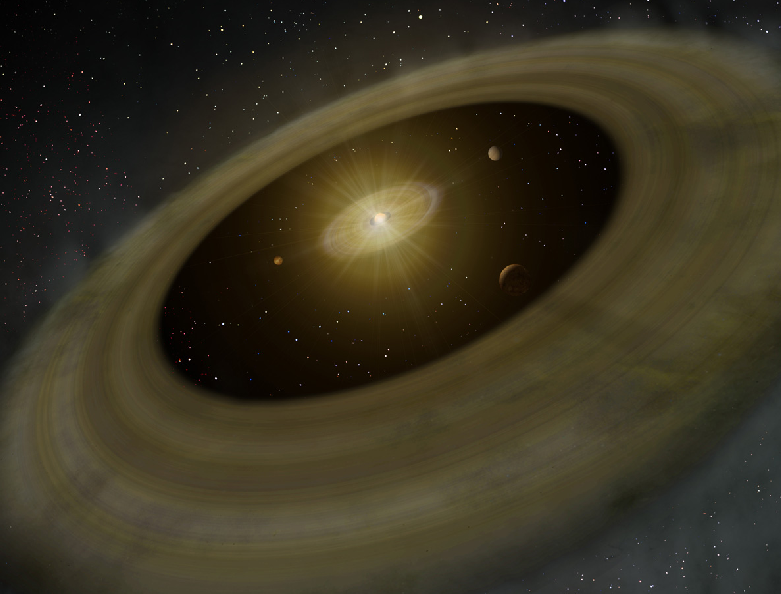
\includegraphics[width=8cm]{frontpage}}

% Use this to make hyperlinks visible in the document.
% \hypersetup{colorlinks=true}

% ---------------------------------------------------------------- My definitions!
% \renewcommand{\vec}[1] {\ensuremath{ \overrightarrow{ #1 } }}
\renewcommand{\vec}[1] {\ensuremath{ \mathbf{ #1 } }}
% \bra \ket \braket and \proj
\newcommand{\bra}[1]{\ensuremath{\langle #1 \vert}}
\newcommand{\ket}[1]{\ensuremath{\vert #1 \rangle}}
\newcommand{\braket}[2]{\ensuremath{\langle #1 \vert #2 \rangle}}
\newcommand{\proj}[1]{\ensuremath{\vert #1 \rangle \langle #1 \vert}}

\newcommand{\kpar}{\ensuremath{k_\parallel}}
% ----------------------------------------------------------------

% \usepackage{tocloft}
% \renewcommand{\cftchapdotsep}{\cftdotsep}
\usepackage{subcaption}
\usepackage{makecell,tabularx}
\usepackage{longtable}
\usepackage{graphicx,wrapfig,lipsum}
\usepackage{caption}
\usepackage[skip=10pt]{subcaption}
\usepackage{mdframed}
%\captionsetup[subfigure]{skip=25pt} % global setting for subfigure

\begin{document}

% roman numbering in the table of contents section
\pagenumbering{roman}

\maketitle

% Table of contents :  it is a good idea to include this into your thesis
\tableofcontents
\cleardoublepage

% The following list of figures and list of tables are optional. Remove the comments if needed
%\listoffigures
%\newpage

%\listoftables
%\newpage

% in the main part of the document use standard arabic numbers. Page counter resets to 1.
\pagenumbering{arabic}
\chapter{Introduction}
One of the biggest questions that arises in each human is how the world around us is formed. It intrigues children already that a pea grows to a complete plant and that their adults were once a child. Much research in astronomy is about how the universe has taken his shape as it is today. How stars, planets and galaxies are formed for example. It has been a question for a long time if the solar system was the only place in the universe to where planets exists. Since then, many indirect methods were developed that could tell if a star hosted planets and the first exoplanet was soon confirmed.
\bigskip

Scientists have made huge progress in the last few decades in understanding the formation of stars and planets. It is now common known that stars are formed by the collapse of a big cloud of gas and dust. The gas and dust that is left in the cloud after the birth of a star starts to fall towards it. This accretion material starts to orbit the star in a plane due to the conservation of angular momentum, forming an accretion disk. In this accretion disks planets start to form when grains stick together to form pebbles, pebbles planeto\"ids and planeto\"ids planets. Another possibility is that the disk gets gravitational unstable, the disk starts to fragment and gas giant planets are formed. %###cite Philip J. Armitage. Astrophysics of Planet Formation. Cambridge University Press, 2010.
\bigskip

The formation of these planets is actually much more complex since there are many processes going on in a disk. Direct imaging of planets and disks has been impossible for a long time, since the contrast between stars and planets is too big and the point spread function (PSF) of the star too much extended. With the development of special optics called coronographs that improve the contrast, special adaptive optics that correct for the distortion of the light in the atmosphere and special techniques to reduce the stellar PSF, we are now able to image planets and protoplanetary disks directly. This provides us detailed information of the conditions in different planetary systems and protoplanetary disk, which improves our understanding of the formation of planetary systems.
\bigskip

SPHERE, one of the instruments of the Very Large Telescopes (VLT) in Chili, was build for direct imaging of planets. This instrument collects high resolution data of exoplanets and circumstellar disk. One mode of the subsystems of the instrument gives light in parallel to IRDIS and IFS. IRDIS is the InfraRed Dual Imaging and Spectograph subsystem that provides classical imaging, dual band imaging, dual-polarization imaging and long slit spectroscopy with a good resolving power, IFS is the Integral Field spectrograph that provides a data cube of 39 monochromatic images \cite{Observatory2007}. Since IRDIS data is easier to reduce and to analyze, and the field of view (FOV) of IRDIS is much bigger than the FOV of the IFS, IRDIS data is much more often analyzed than IFS data. Since there exists as much IFS data as there exists IRDIS data, much of the disk data made by IFS is still unpublished.
\bigskip

Since the IFS can provide a resolved spectrum of an object, it is possible to get a spectrum of a protoplanetary disk. Untill now, we do not have detailed information about the colour of the object that mainly will be analyzed in this project, the disk around T-Tauri star RX J1615.3-3255 (RX J1615). Reliable spectral information of protoplanetary disks can lead us in the future to a better understanding of ongoing planet formation in protoplanatary disks in general, since resolved spectral data of a disk can tell us something about the grain properties in different regions of the disk. This could provide us a better feeling of the requirements for a planet to form in protoplanetary disks and the way planetary system as our solar system are formed. 
\bigskip

There are many steps to make for this to achieve. One of the first steps is a good reduction of the raw data. One of the main goals of this research is hence to investigate what the best way is to reduce the raw data: what calibration data is needed and which calibration steps there have to be taken. There are various effects at play that we want to understand if we have this basic reduction done. It appears that the disk gets better detected at longer wavelengths. One of the goals of the project is to check if this is a property of disks, or that this is only an effect of the adaptive optic performance getting better at longer wavelengths, which it generally does. By use of different post-processing techniques the starlight can be subtracted in order to detect the disk, but these techniques can effect the spectrum and the morphology of the disk. One goal of the project is hence to check how strong these effects are and what we can trust out of the data.
\bigskip

\chapter{Theory}
\section{Protoplanetary disks}
\begin{wrapfigure}{R}{0.35\textwidth}
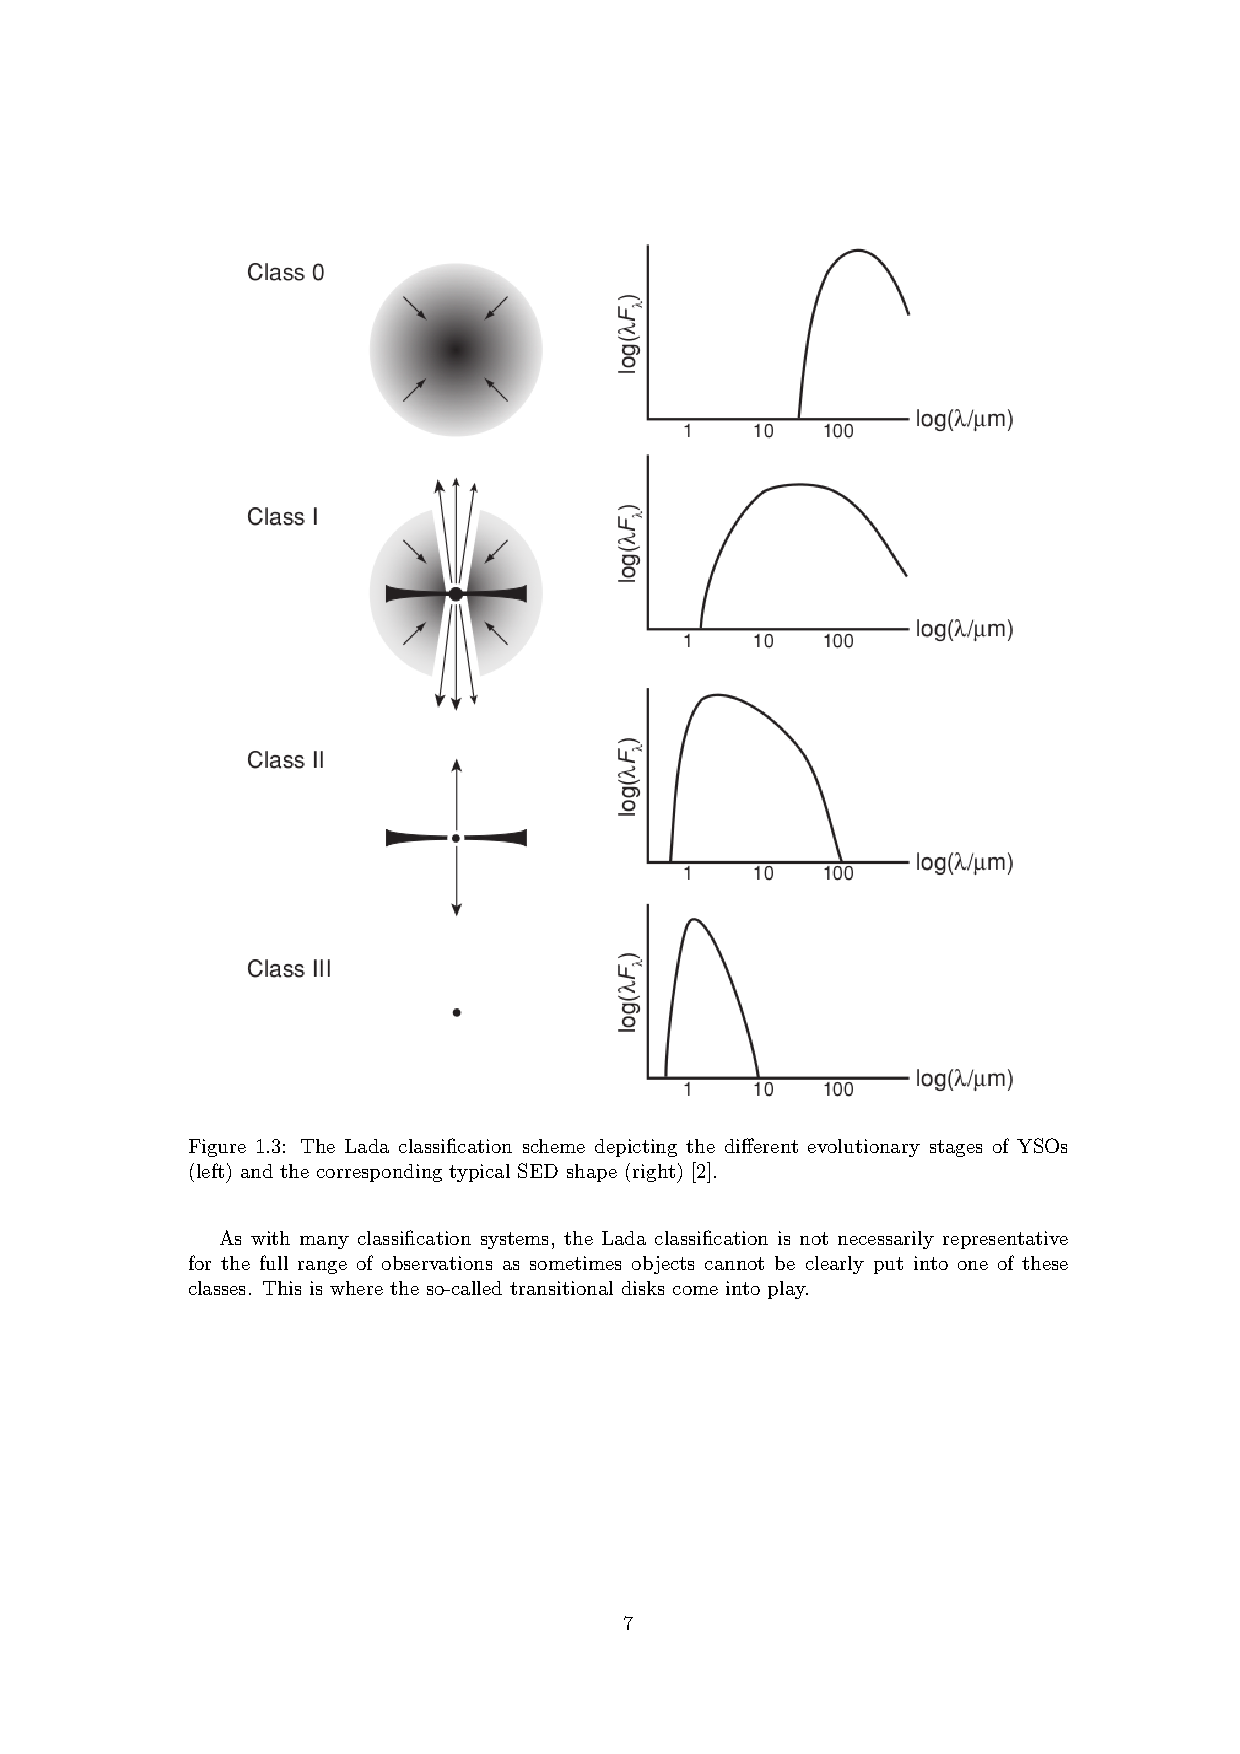
\includegraphics[trim={4cm 11cm 11cm 4cm},clip,width = 0.35\textwidth]{classscheme}
\caption{The four classes of young stellar objects (YSO), from top to bottom: a cloud collapses into a protostar (Class 0), a disk starts to form by conservation of angular momentum (Class I), the outer envelope dissipated, the protostar is now only surrounded by a disk (Class II), the disk gets optically thin and a star with possibly a planetary system is left (Class III)}
\vspace{-60pt}
\label{fig:classscheme}
\end{wrapfigure}%

The formation of a star with a planetary system as the sun has multiple stages. The youngest stars are still embedded in the molecular clouds where they form from gravitational collapse of interstellar gas. Older disks are gravitationally stable and have been cleaned over time by planets. protoplanetary disks evolve by two meganisms: infalling gas and dust, known as viscous accretion which transports the angular momentum and photoevaporation. The evolution of protoplanetary disks is classified in four different classes, according to the scheme that Lada introduced in 1987, as illustrated in Figure \ref{fig:classscheme}. 
\bigskip

The youngest stars are found in Class 0. They have a massive accretion disk that is indistinct of the dense envelope. All the light of the protostar is absorbed by this accreting envelope, making these objects invisible in the optical. These objects were first no part of the classification because they were first discovered decades later when the first infrared and millimeter telescopes were built.
\bigskip

The objects in Class 1 have a distinct disk and get more visible in the optical, since the star in the center is less obscured by the decreasing density of the envelope. Since the density in the disk increases, the temperature rises and the peak of the emission of the disk starts shifting to the mid-IR. Objects in this class could also eject collimated jets with a high velocity from the poles. These jets are formed as a byproduct of the accretion process and could influence the evolutionary track of the object.
\bigskip

The envelope is totally disipated for Class 2 objects and the star is only surrounded by an optically thick accretion disk. These type of objects are also known as T-Tauri stars, named after the prototype T Tauri, if they have a mass smaller smaller than 2 $M_\odot$. These objects are all younger than 10 million years old. Analogs of these stars, but with a higher mass than 2 $M_\odot$ are called Herbig Ae/Be stars. 
\bigskip

The disk in Class 3 objects has dissipated, leaving the protostar with an optically thin debris disk and a possible planetary system. The SED no longer contains a disk component at longer wavelength, but is totally dominated by the light of the protostar. This class ends when the nuclear fusion in the core of the protostar starts and the protostar becomes a main sequence star.
\bigskip

Objects in the stage between Class 2 and Class 3 are called transition disks. These stars  have more than just a debris disk, but the disk starts to get less prominent. Some disks have a cleared region, close to the star. This part is heated the most by the star. This cleared region is often called a gap. Inside the cleared region an inner disk can be present as a remnant from the optically thick accretion disk.

\section{The object}
R band magnitude + spectral type

The main object of study is the disk around T-Tauri star RX J1615.3-3255 (hereafter RX J1615). RX J1615 is a star in the scorpius constellation on the southern hemisphere, with co\"ordinates 16 15 20.231 -32 55 05.10 and a member of the Lupus star forming region. The distance to this region is previously estimated to be 185 kpc \cite{Krautter1997}. The mass of RX J1615 is previously determined to be 1.1$M_\odot$ and the age 1.4 Myr\cite{Wahhaj2010}. 


\begin{wrapfigure}{R}{0.5\textwidth}
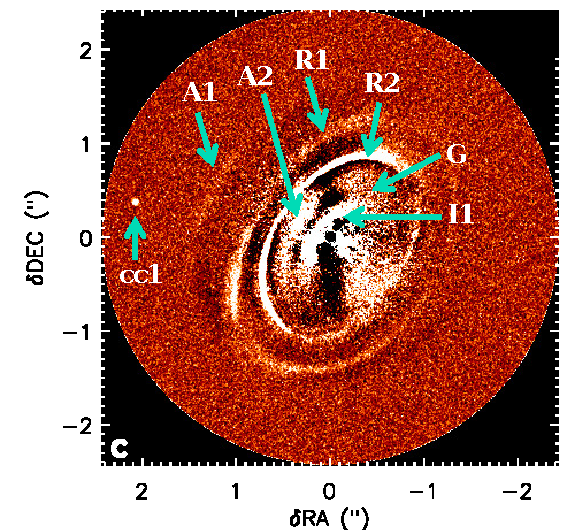
\includegraphics[width = 0.5\textwidth]{irdisjos}
\caption{Reduction of IRDIS ADI data. From the outside in, companion candidate (cc1), arc (A1), two full rings (R1 and R2), another arc (A2), a gap (G), and an innermost disk structure (I1)\citep{DeBoer2016}}
\label{fig:irdisjos}
\end{wrapfigure}

\noindent
It is well known that this star hosts large circumstellar disk structures.  As illustrated in Figure \ref{fig:irdisjos}, there are two different rings detected in IRDIS data (R1 and R2) at $278\pm 2$au and $196\pm 2$au, an inner disk component (I1) at $56\pm 2$au and two arcs (A1 and A2). A2 is confirmed to be a full ring, but the detections have not been deep enough to determine the origin of A1, it could either be a seperate ring or the backward facing side of R1 \citep{DeBoer2016}. In the rest of the document these abbreviations will be used to indicate which part of the disk signal is meant.
\bigskip

A reduction of IFS T-LOCI ADI data, taken in the Y-J range, is already available of the same dataset, Figure \ref{fig:ifsjos}. Template Locally Optimized Combination of Images (T-LOCI) is an advanced way of selecting regions to make a reference to subtract the point spread function of the star from the data, but conserving the signal of the disk in the data. In this data one ring (corresponding to R1 in Figure \ref{fig:irdisjos}) and small signal of the inner disk component (I1) and the arc closest to the star (A1) are detected.

\begin{figure}[ht]
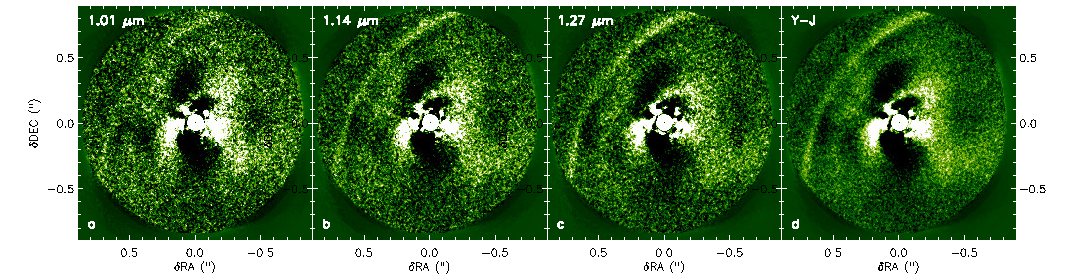
\includegraphics[width = \textwidth]{ifsjos}
\caption{Reduction of IFS ADI data. From left to right: \textbf{a:} median of the first 13 channels (0.96-1.07$\mu m$) \textbf{b:} median of 13 channels (1.08-1.21 $\mu m$) \textbf{c:} median of 13 channels (1.22-1.33 $\mu m$) \textbf{d:} median of the entire YJ range \citep{DeBoer2016}}
\label{fig:ifsjos}
\end{figure}

RX J1615 is also resolved with the Submillimeter Array (SMA) at 880 $\mu m$ (Andrews) and with the  Atacama Large Millimeter/submillimeter Array (ALMA) 690 GHz continuum data (van der Marel). IRDIS and IFS detect scattered Near InfraRed (NIR) light of the disk, emitted by the star. These infrared observations, however, say something about the emission of the gas and dust of the disk itself, mainly coming from the core or mid-plane of the disk where the pressure of the gas and dust is relative high. Both observations show a cavity up to 20-30 au, confirming that RX J1615 has a transition disk. 

\begin{figure}[htb]
\centering
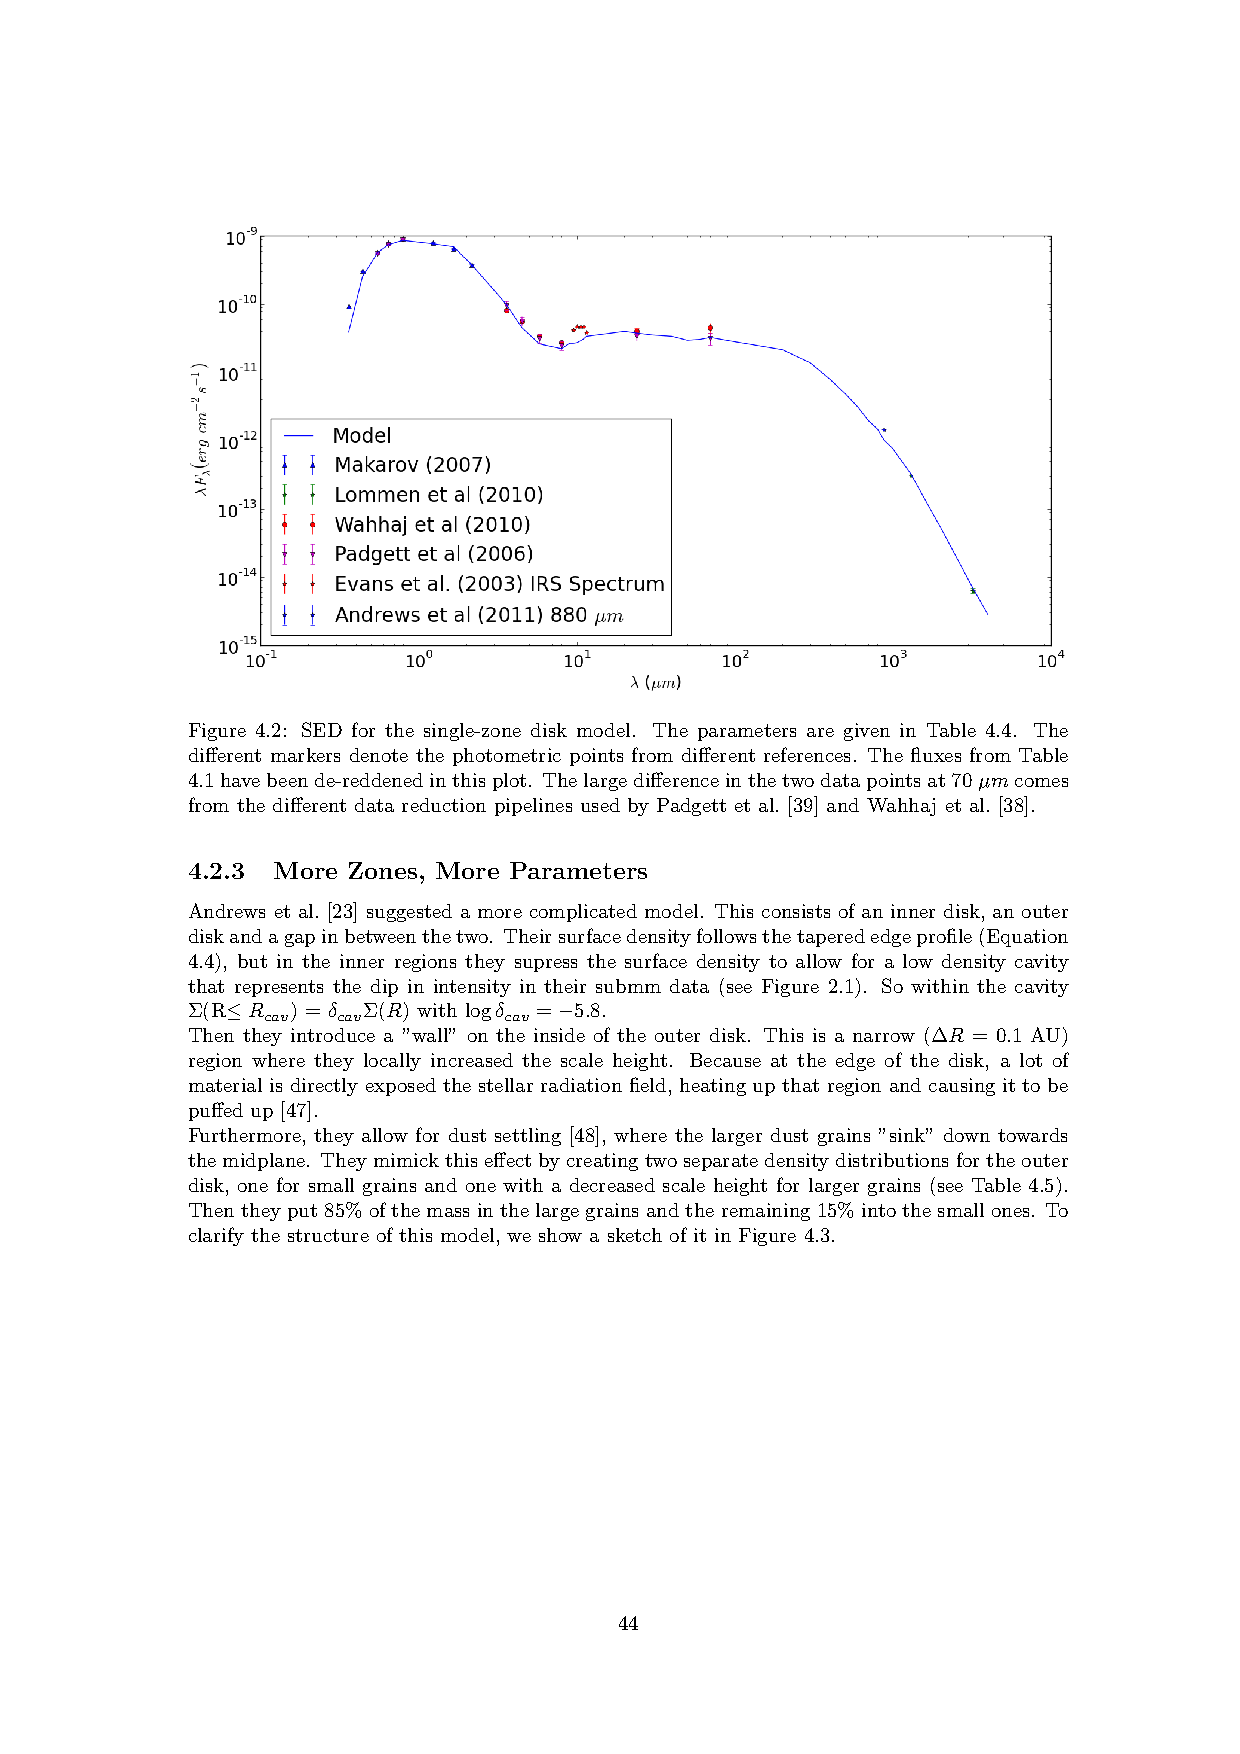
\includegraphics[trim={2cm 18cm 2cm 3.7cm},clip,width = \textwidth]{SED.pdf}
\caption{The spectral energy distribution of RX J1615. The contribution on the left is due to stellar flux, the contribution to longer wavelengths is due to flux of surrounding structures \cite{thesis2014}.}
\label{fig:SED}
\end{figure}

The spectral energy distribution (SED) of the star as determined by different research groups is illustrated in Figure \ref{fig:SED}. This figure displayes the contribution in flux of the object over the whole spectrum. The flux of the protostar is responsible for the contribution on the lower end of the SED. This contribution look like a blackbody spectrum with a temperature of about 1900K, peaking around the H-band \citep{Padgett}. The slowly decreasing part on the high end of the SED is due to signal of the disk. The disk is mostly radiating in the infrared, due to its much lower temperature.

\chapter{Instrumentation}
\section{SPHERE}
\begin{figure}[hb]
\centering
\begin{subfigure}{.58\textwidth}
  \centering
  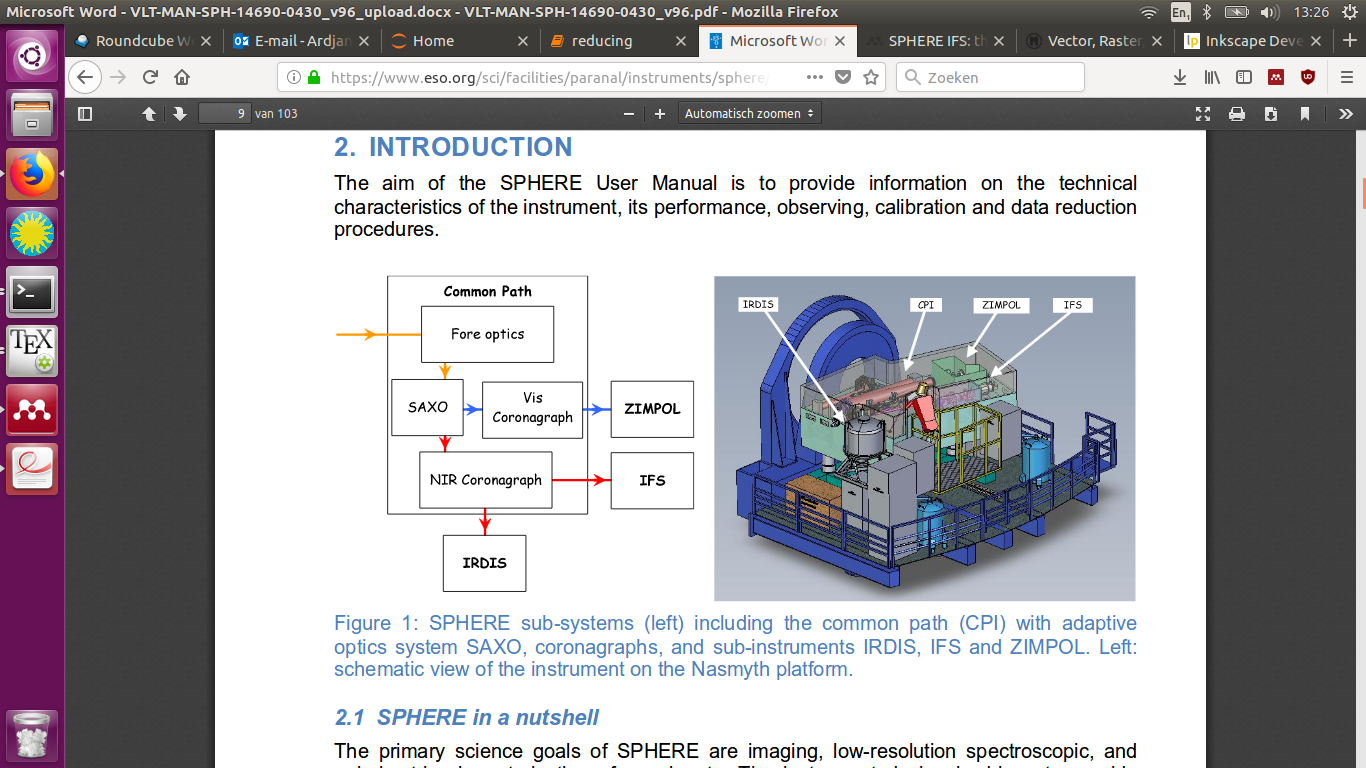
\includegraphics[trim={25cm 6cm 7cm 8.8cm},clip,width = 1\linewidth]{overviewSPHERE}
  \caption{\citep{Observatory2007}}
  %\label{fig:sub1}
\end{subfigure}\hfill
\begin{subfigure}{.38\textwidth}
  \centering
  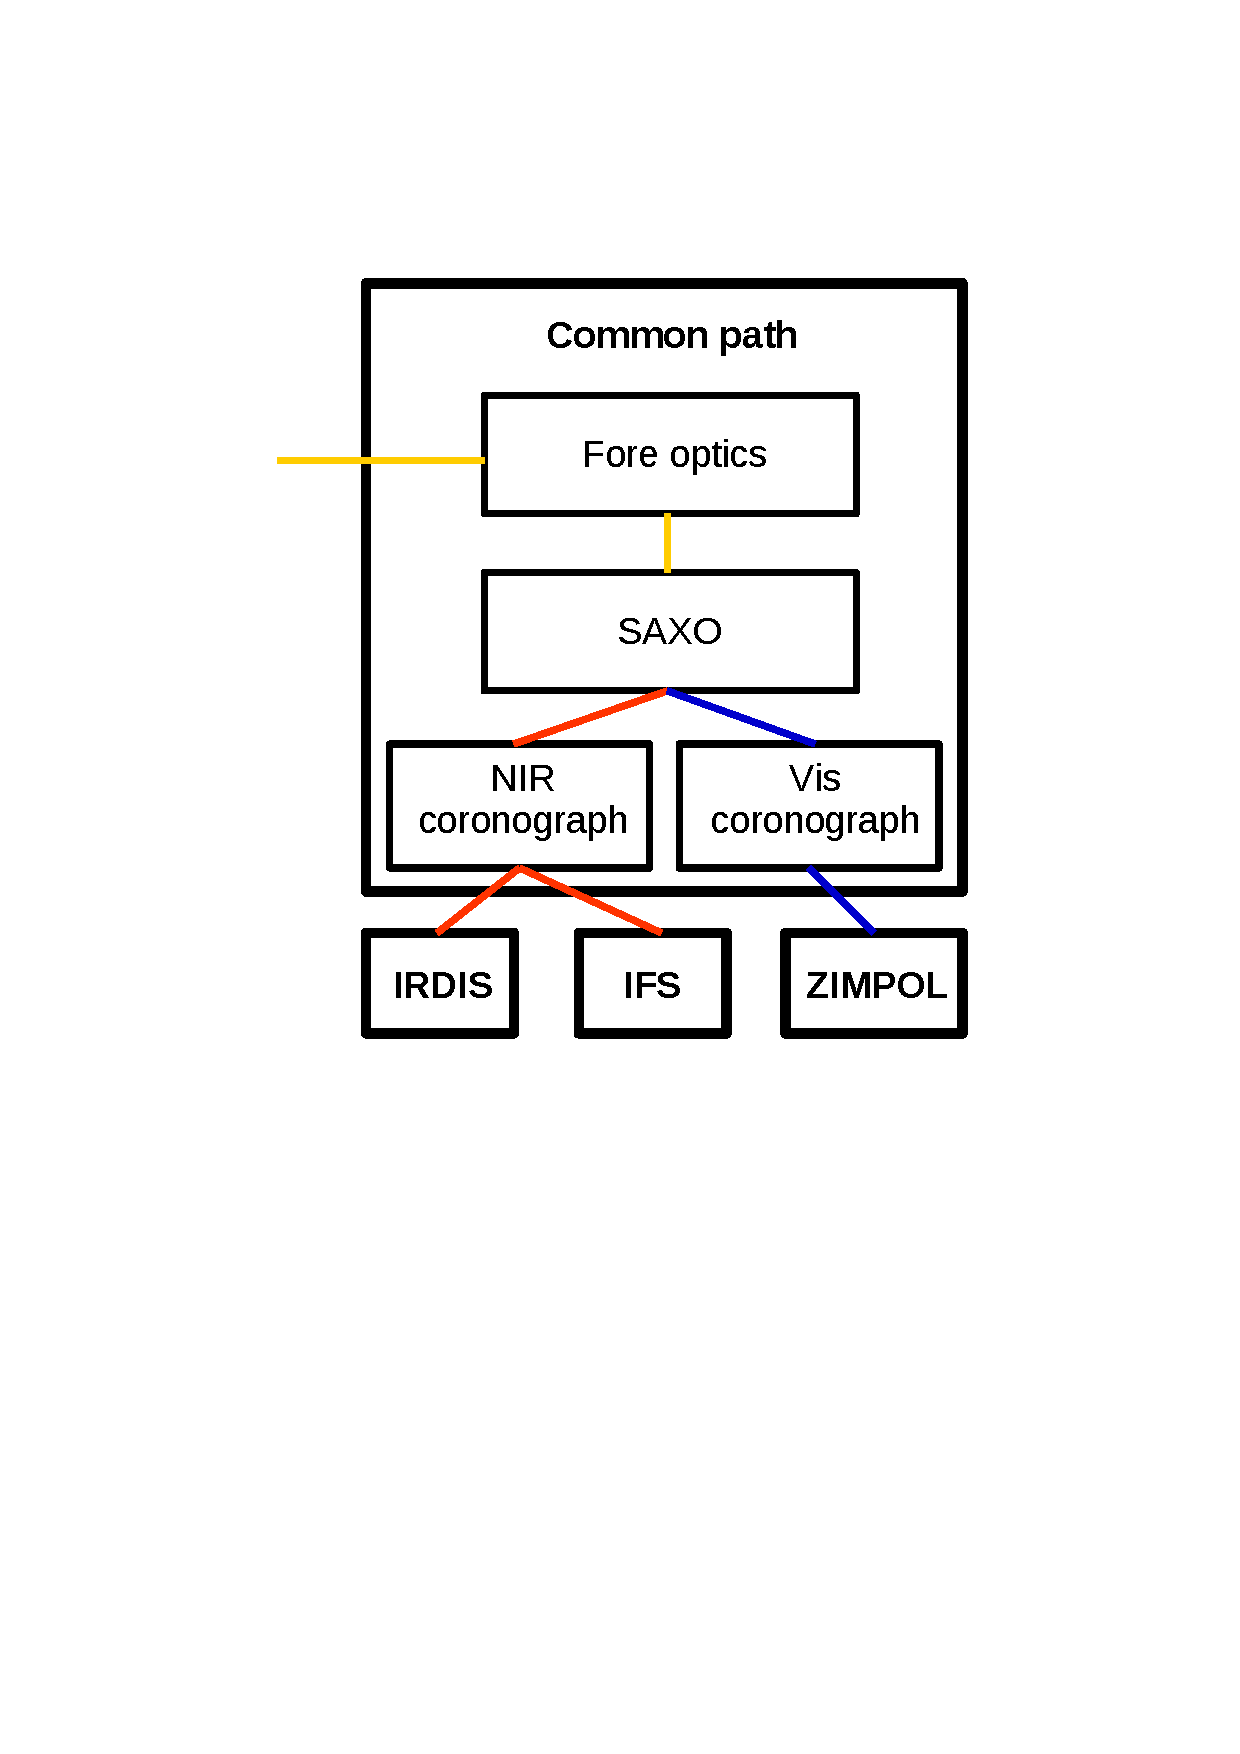
\includegraphics[trim={5cm 12cm 3.5cm 3.5cm},clip,width=1\linewidth]{overview_SPHERE}
  \caption{}
  %\label{fig:sub2}
\end{subfigure}
\caption{overview of SPHERE}
\label{fig:overviewSPHERE}
\end{figure}

SPHERE, (Spectro-Polarimetric High-contrast Exoplanets REsearch) is an instrument for the VLT which is optimized for high contrast imaging. The instrument is placed in the Nasmyth  of Unit Telescope 3 (UT3), one of the main VLT units, as illustrated in Figure \ref{fig:overviewSPHERE}. The instrument can be split up into four systems, the common path optics and three subsystems, IRDIS, IFS and ZIMPOL. ZIMPOL uses visible light and IRDIS and IFS both near infrared light (NIR). Since IRDIS and IFS can work at the same time, by guiding a part of the spectrum to the IFS and a part to IRDIS by use of a dichroic, we will discuss IRDIS briefly and take some time to look at the IFS in detail.

\subsection{Common path}
The common path interferometer (CPI) is the main system of SPHERE that powers all the cryostats and motors, corrects the light for many distorsions and connects all the sub-systems to the light path. The common path can also include coronographs in the light path. SAXO, the Sphere Adaptive optics for eXoplanet Observation 

\subsubsection{pupil stabilizing fore optics}
SPHERE has a derotater that is able to stabilize the field or the pupil on the detector. This stabilization is needed because of the rotation of the earth around its axis. This rotation of the earth causes a rotation of the field due to a change in parallactic angle and altitude of the object and a rotation of the pupil that is only due to the change in altitude of the object that is observed. This derotator can also switched of in order to take data which can be used in angular differential imaging routines. The pupil has an offset with respect to the true north of -135.99$^o$, which means that all the data taken with SPHERE has to be rotated with that angle in order to make sure that north is pointing up in the data. The field of view of the IFS is for technical reasons rotated with respect to the IRDIS field of view by 100.48$\pm$0.10$^o$. IFS has an aditional derotator to align the north up. But if the derotators are turned off in observations, which was the case in our data, providing a possibility to do angular differential imaging, the data has to be rotated with the offset in order to make sure that the north is pointing up. %###\cite{maire} 
\bigskip

After entering the instrument, the light path is protected against many possible noise sources. The vibrations in the Nasmyth platform that are caused by seismic activity or other reasons are damped by use of servo-controlled pods and the whole instrument is protected against changes in temperature and dust by a protective cover. The light is then propagated in the complete spectral range from 0.450$\mu m$ to 2.320$\mu m$ to the beamsplitter that splits the light in a visible part for ZIMPOL, the polarimetric subsystem that works in the visual range and a near infrared (NIR) part for both IRDIS and IFS. If ZIMPOL is not used, all that light goes to the wavefront sensor that is used by the adaptive optics system to correct for the aberations of the light in the atmosphere. After the dichroic, the light is guided through an atmospheric dispersion corrector (ADC) that corrects for dispersion effects in the atmosphere, due to changes increase in altitude of the object.
\bigskip

\subsubsection{adaptive optics}
Sphere AO for eXoplanet Observation (SAXO) is the adaptive optics module of SPHERE. It is composed out of different components, each correcting a part of the distortion of the light. The bundled information fo these components is send to the deformable mirror (DM), that corrects for phase perturbations of up to a frequency of 1.2 kHz by use of the 41x41 actuators that are able to deform the mirror \citep{Observatory2007}. The phase perturbations are measured by different components.
\bigskip

\begin{figure}[htbp]
\centering
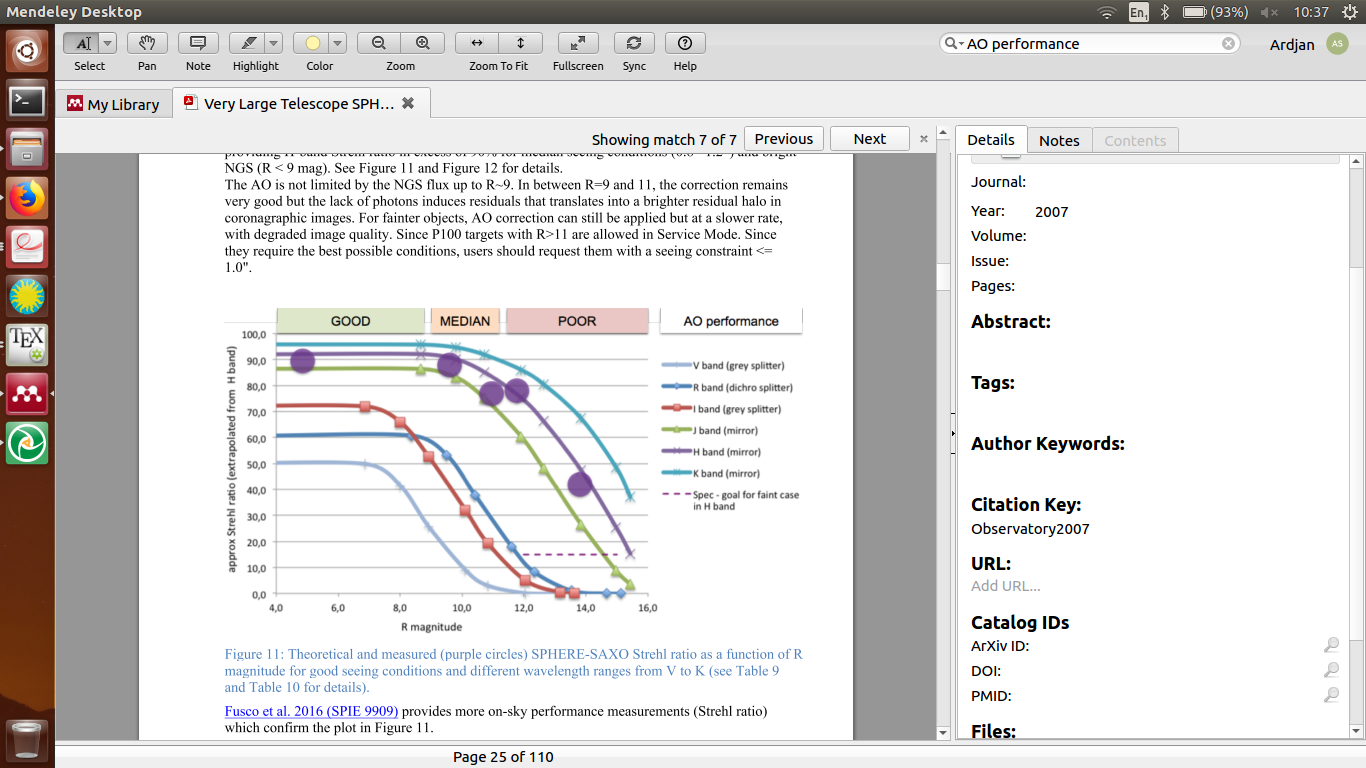
\includegraphics[trim={7cm 4.5cm 19cm 10cm},clip,width = 1\textwidth]{aoperformance}
\caption{Theoretical and measured (purple circles) SPHERE-SAXO Strehl ratio as a function of R magnitude for good seeing conditions and different wavelength ranges from V to K\citep{Observatory2007}}
\label{fig:aoperformance}
\end{figure}

The turbulence is measured by a wavefront sensor that transposes the phase shift to an intensity distribution on a detector. The wavefront sensor that is used is a 40x40 lenslet Shack-Hartmann sensor. (ANUGU!!!!) This sensor uses a lenslet array that produces a spot on a detector for each lenslet. A distorted incomming wavefront changes the position of the focal spot of a lenslet on the sensor. From these positions the local tilt of the wavefront can be calculated. Other distorsions such as image motion, pupil shift and distorsion in the instrument are measured with tip tilt sensors and corrected by the DM, correcting the only the large scale differences that these distorsions cause.
\bigskip

The wavefront of the object that is incomming, is accurately corrected in a radius of about 20 $\lambda/D$ in the image plane. Further out is the PSF still corrected, but not enough to suppress the stellar halo. The correction of the AO is dependent of the R magnitude, since the Shack-Hartmann sensor measures the perturbations of the wavefront in the range of the R filter. The more light is provided to the sensor, the more accurate the distorsions of the wavefront can be measured \ref{fig:aoperformance}, which could drastically change the overall performance of the AO and hence the quality of the data.

\subsubsection{coronographs}
A coronagraph is a device that increases the contrast between the star in the central and the background by surpressing the PSF that is produced by the star. SPHERE has several coronagraphs for different conditions the instrument can work. All coronagraphs consist of three components. At the begin of the light path an apodizer changes the beam profile and improves the dynamic range of the image that way. Further downstream focal plane masks shift the phase of the image in one of the foci of the instrument, creating a self-destructive interference that blocks most of the light of the star.  Behind the focal plane mask a Lyot pupil stop reduces the flare in te system, meaning that reflected and scattered light on the different optical components is left out of the image. Different combinations of these three elements have different results on the final image and all the combinations have conditions they work the best. Think of the wavelength range at that moment is used, seeing and needed inner working angle.

\subsection{IRDIS}
IRDIS is the InfraRed Dual Imaging and Spectograph subsystem that works in the NIR. IRDIS has a field of view of 11" x 12.5" and has several modes in which data can be acquired. IRDIS provides classical imaging, dual band imaging, dual-polarization imaging with the filters Y to Ks and long slit spectroscopy if it used alone. There are also two modes wherein IFS and IRDIS take data in parallel. This can be achieved by the use of dichroic filters that let light in a certain wavelength range pass and reflects the other light. If the instrument is set up in IRDIFS mode, the IFS gets all the light in the Y-J band and IRDIS is able to do narrow band or broad-band H Dual band imaging in parallel. In the IRDIFS\_EXT mode, the IFS get the light in the range from Y band to H band, leaving IRDIS with the possibility to get dual band imaging data with lower efficiency in a narrow-band filter or in broad-band K. The end-to-end efficiency of both possibilities are shown in Figure \ref{fig:systemthrougput}. 

\begin{figure}[htbp]
\centering
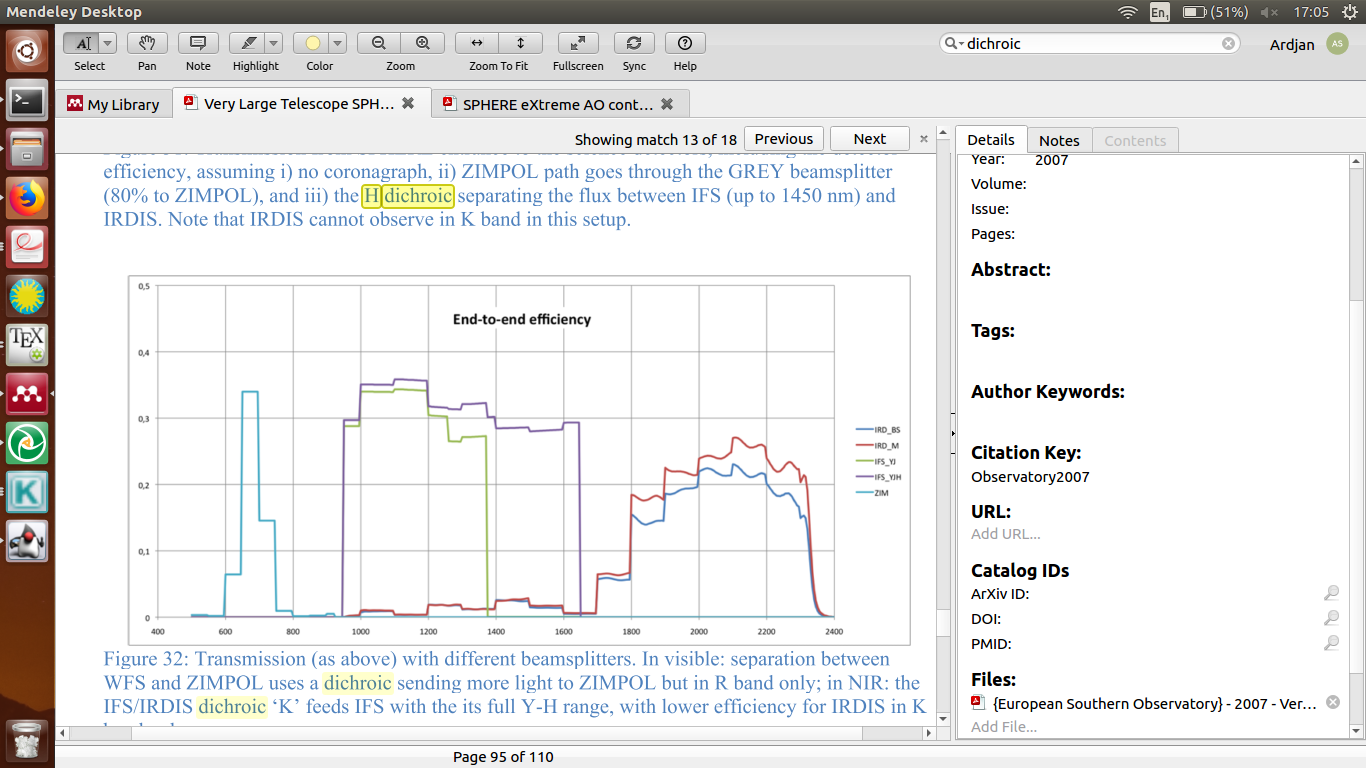
\includegraphics[trim={4cm 4.3cm 16cm 9cm},clip,width = \textwidth]{systemthroughput}
\caption{End-to-end efficiency if both IFS and IRDIS get light. The light of ZIMPOL is in this case for the AO system.}
\label{fig:systemthrougput}
\end{figure}

\section{Integral Field spectrograph}
\begin{figure}[htbp]
\centering 
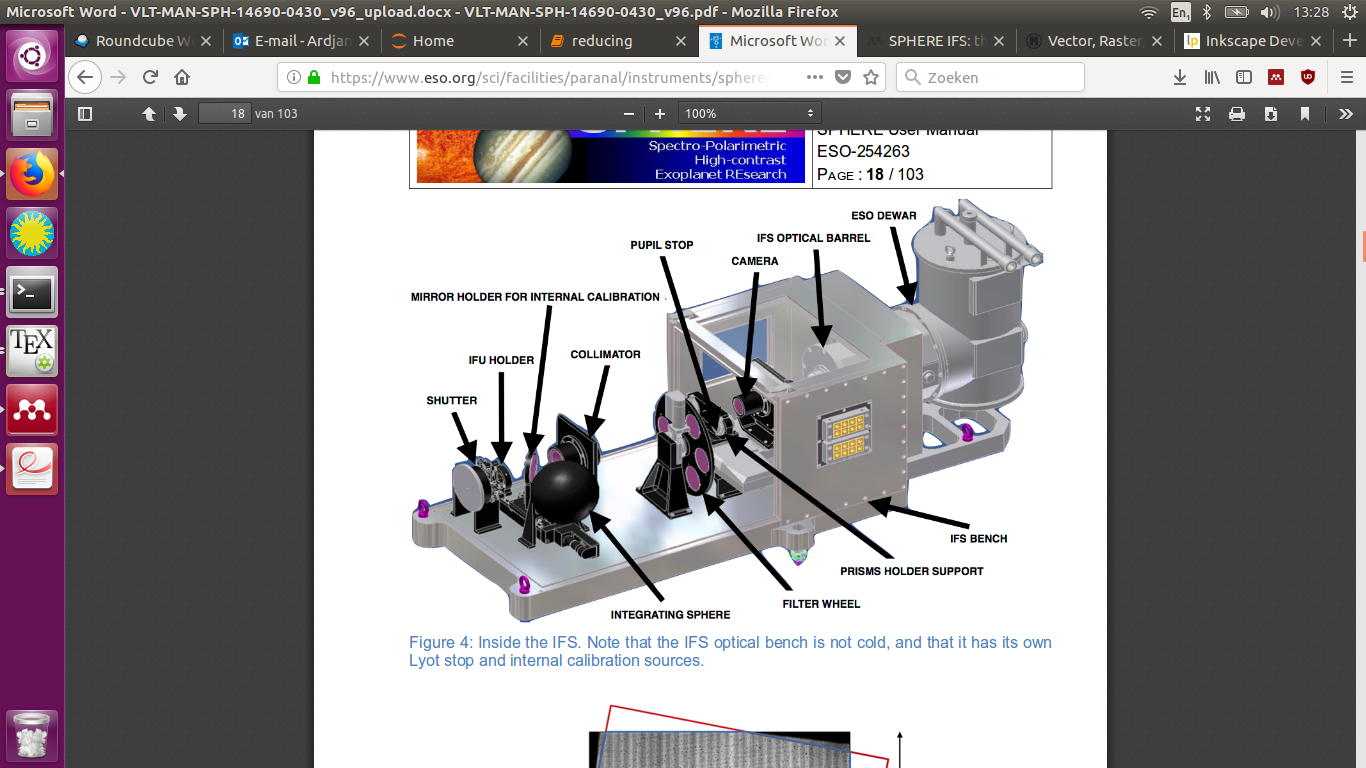
\includegraphics[trim={13cm 5cm 10cm 7cm},clip,width = 0.6\textwidth]{overviewIFS}
\caption{Overview of the IFS\cite{Observatory2007}} 
\label{}
\end{figure}

The integral field spectrograph is a subsystem of SPHERE that is able to collect data over a wavelength range from 0.95 $\mu m$ up to 1.346 $\mu m$ or 1.677 $\mu m$, depending on the mode (Y-J or Y-H) the instrument is in. The IFS receives stable light, which is corrected for many distorsions in the common path and at the deformable mirror. The IFS has a total field of view of 1.73" x 1.73", so much smaller than IRDIS', but enough to be able to detect inner structures of protoplanetary disks. IFS focuses on the NIR because that is the range in which the most useful broad molecular bands of the planets are expected to show off.

\subsection{IFU unit}
\begin{wrapfigure}{R}{0.6\textwidth}
\centering 
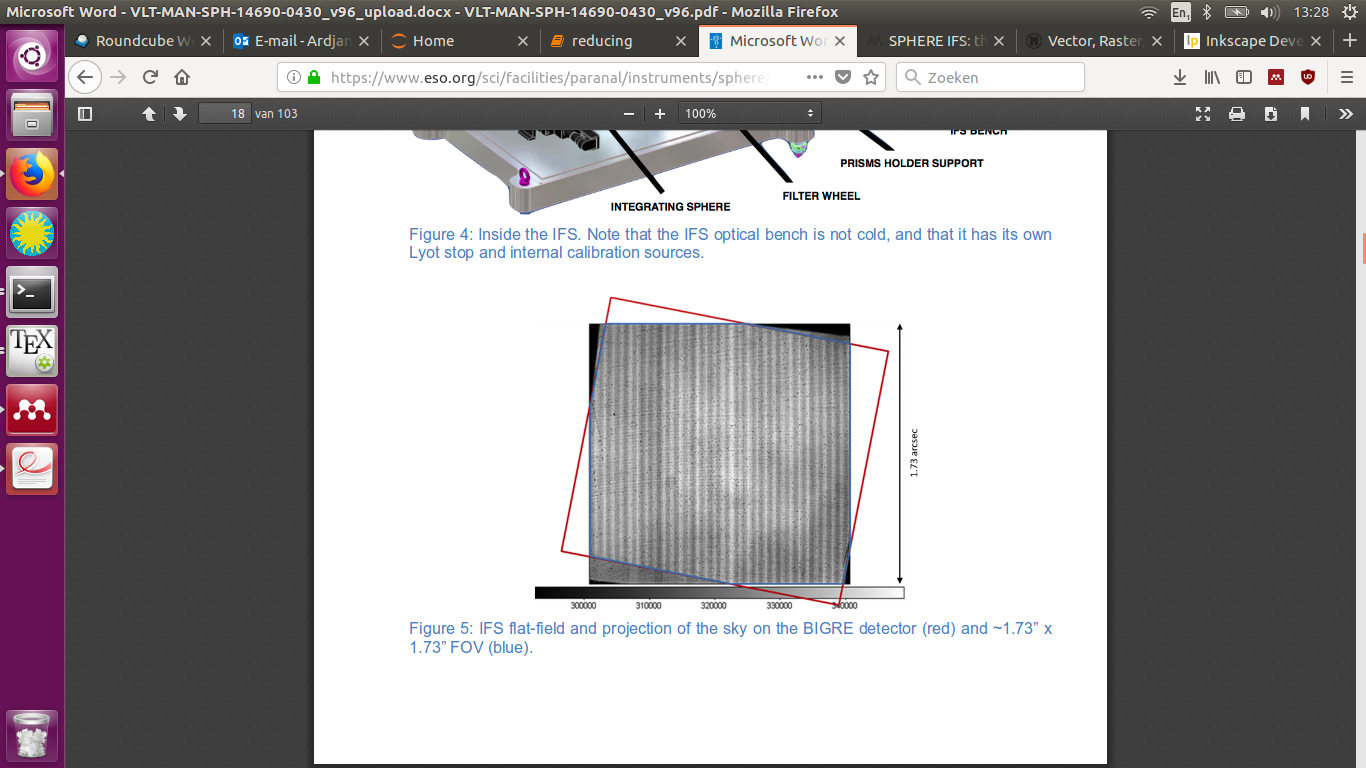
\includegraphics[trim={15cm 5.5cm 10cm 9.5cm},clip,scale = 0.47]{biggre}
\caption{IFS flat-field and projection of the sky. In the red the arrangement on the BIGRE detector and in blue the useful FOV. \citep{Observatory2007}} 
\label{fig:bigre}
\end{wrapfigure}

The IFS is able to obtain spectral information by use of BIGRE, an integral field unit consisting of 21000 microlenslets in a hexagonal grid, as illustrated in Figure \ref{fig:bigregrid}. This grid is rotated by $10.7^o$ with respect to the dispersion in order to get the most lenslets stacked on the grid. This causes that a small section of the detector is meaningless, Figure \ref{fig:bigre}. The spectra of these lenslets are projected on the detector in a rectangular area with dimensions 5.1 x 41 pixels. 


\begin{figure}[htbp]
\centering 
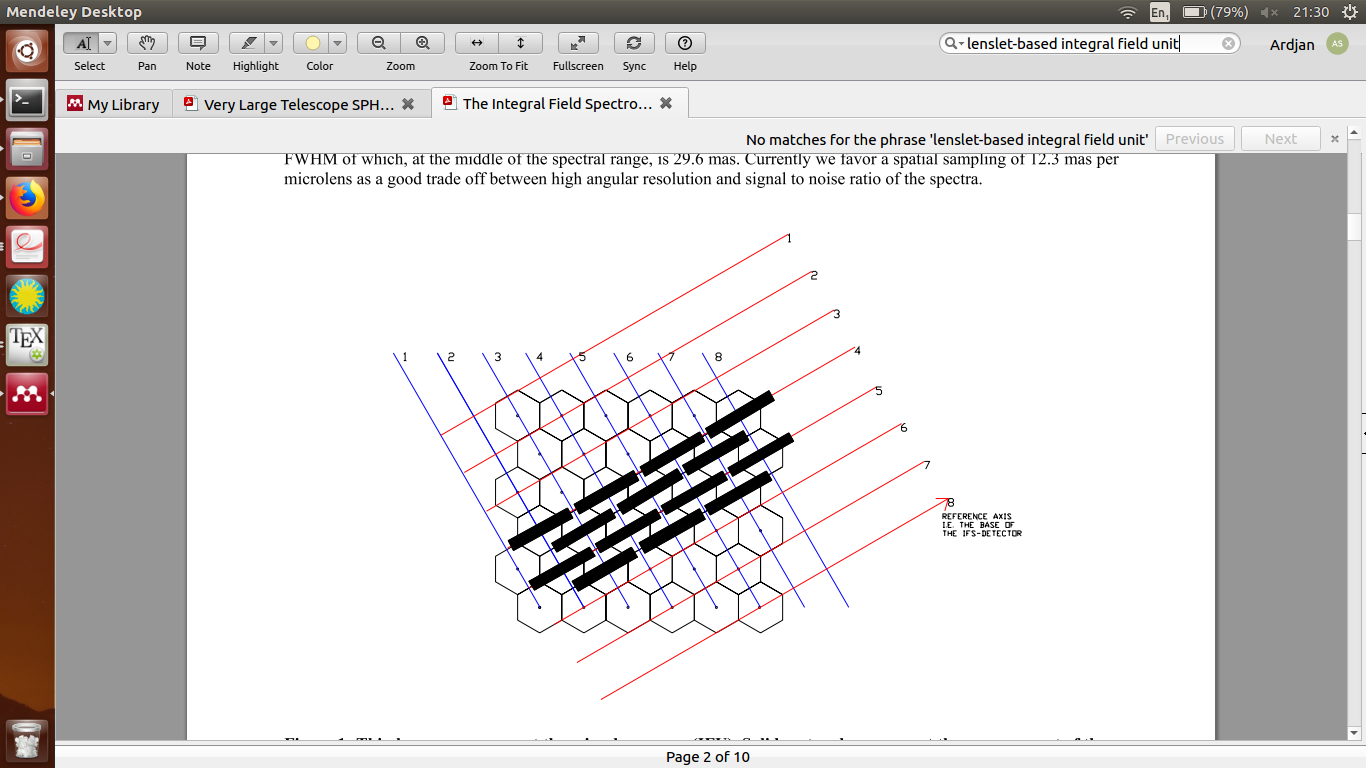
\includegraphics[trim={15cm 1.5cm 10cm 8cm},clip,scale = 0.47]{bigregrid}
\caption{The hexagonal lines represent the different microlenses of the IFU, the solid rectangles represent the spectra of the lenslets on the detector. The numbered lines  represent the orientation of the IFS Detector \cite{Claudi2008}} 
\label{fig:bigregrid}
\end{figure}

\subsection{Detector}
The detector of the IFS is 2048x2048 pixels. It is a standard infrared detector, since all light with a longer wavelength than the biggest wavelength in that mode is blocked. This light is blocked by use of a filter that has a sharp cut-off at the desired wavelength. It is technically possible to block longer wavelengths by us of the cut-off wavelength at which an HgCdTe detector is no longer sensitive, but this would make the instrument unnecassary complex and would increase the readout noise drastically from ~10 $e^-$ to ~25$e^-$\citep{Claudi2008}.
\bigskip

The detector is cooled with liquid Nitrogen, which reduces the thermal noise of the detector. The thermal noise of the cooled detector can be neglected with respect to dark noise in the instrument, photon noise of the observed star and other noise sources\citep{Claudi2008}. The detector is static and does not need to be rotateble since the rotation of the field and the pupil are corrected in the derotator. 

\subsection{Calibration devices}
The IFS has two calibration arms to provide a proper calibration of the instrument. The first arm is mounted in the common path and consists of a few calibration lamps. These lamps can be used to measure the througput of the lenslet grid and the different optical components in the IFS itself. Four additional lasers with wavelengths of respectively 0.9877, 1.1237, 1.3094 and 1.5451($\mu m$) are also provided on this calibration arm for the wavelength calibration. Each of the lasers is focused by the IFU on a different part in the spectra on the detector. Interpolation between these points gives an accurate model for the wavelength solution for each pixel, which can be used to reduce the data.
\bigskip

The second calibration arm is mounted internal to IFS, after the IFU, such that flats can be taken that measure the sensitivity of the whole detector. This is not possible with the external calibration lamps, since the detector has bigger dimensions than the FOV of the lenslet grid. decoupling the noise of the IFU and the detector makes the calibration slightly better and this allows to take calibration frames simultaneously to IRDIS, making the process of taking calibration data much faster. The internal calibration arm consist out of five calibration lamps: four narrowband lamps, centered around 1.0, 1.2, 1.3 and 1.5 $\mu m$, with a full width half maximum (FWHM) of about 0.01-0.04 $\mu m$ and one broadband white lamp\citep{Desidera}. An integrating sphere is also provided that spreads the light of the different lamps evenly over the whole detector.

\chapter{Methodology}
\section{IFS reduction for dummies}
Data taken with an integral field spectrograph contains for each pixel a spectrum, as illustrated in Figure \ref{fig:rawdata}. To reduce this to a cube with a frame for each wavelength bin as illustrated in Figure \ref{fig:reduceddata}, several calibrations were needed. At first the dark current had to be subtracted and all pixels had to be corrected for their sensitivity using detector flat frames. After that the different spectra had to be located and the wavelength of all pixels calibrated. 

\begin{figure}[hb]
\centering
\begin{subfigure}{.48\textwidth}
  \centering
  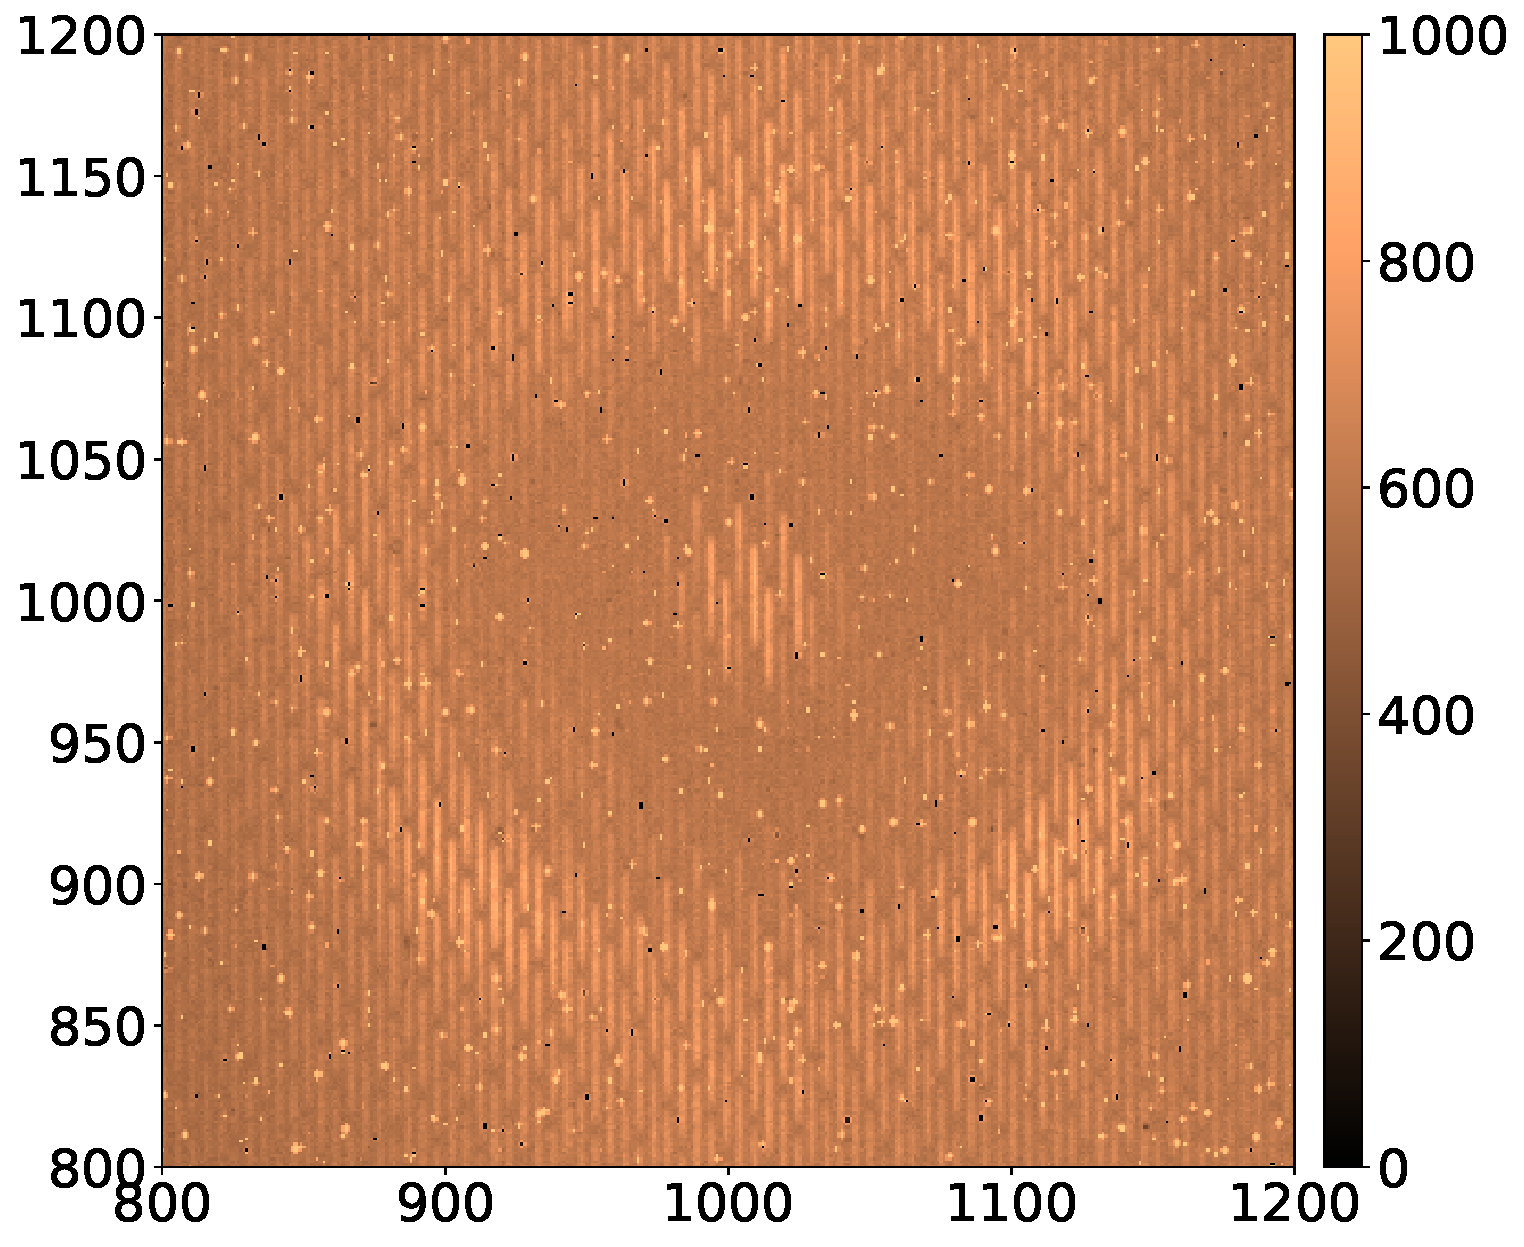
\includegraphics[width=1\linewidth]{rawframe}
  \caption{zoom of one of the raw science frames}
  \label{fig:rawdata}
\end{subfigure}\hfill
\begin{subfigure}{.48\textwidth}
  \centering
  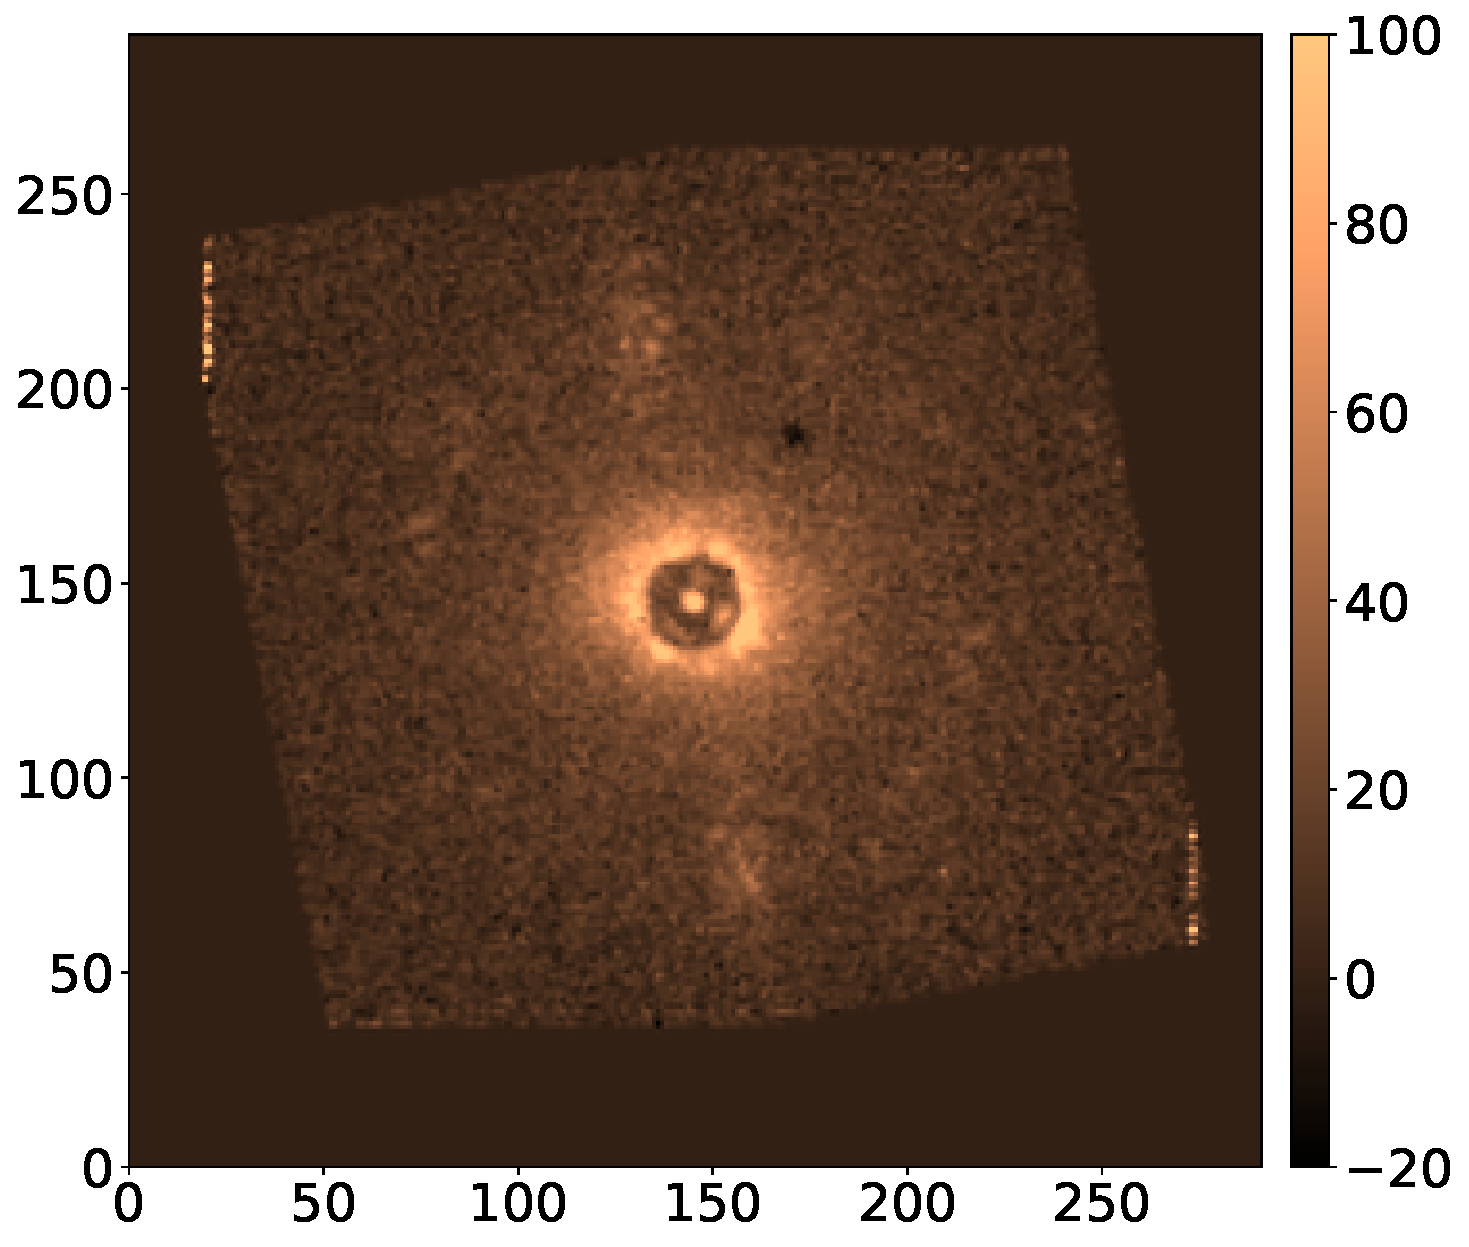
\includegraphics[width=1\linewidth]{reducedframe}
  %\hspace{7 mm}
  \caption{one of the 39 wavelength slices of a reduced science frame}
  \label{fig:reduceddata}
\end{subfigure}
\caption{the result of the basic reduction}
\label{fig:datareduction}
\end{figure}

After correcting for the througput of the lenslet grid, the science reduction produced the final result with 39 spectral channels, each with a dimension of 291x291 spaxels.
\bigskip

The Common Pipeline Library (CPL)\citep{Observatory2007} is a library of commands that is able to do the basic reduction steps of SPHERE data. Running the CPL can be done by use of Esorex, which is a commandline driven package, or EsoReflex that provides an easy and flexible way to run the different recipes of the pipeline. Esorex requires the use of a set of frames (sof) file for each recipe. This can easily be automized using Python, but since it is much work to write a code that identifies the different calibration images and mistakes can easily be made in the selection of the required data, I have used EsoReflex for the reduction and I really recommend using EsoReflex in the future. EsoReflex provides a user interface in the form of a workflow with a setup of a basic reduction pipeline in advance, which can be adapted in an easy way. It identifies all the required data that is unsorted stored in the input directory and gives a warning if something is missing. 
\bigskip

The data needed for a basic reduction is listed in table \ref{Tab:data}. Note that all the data has to be taken in the same mode, YJ or YH, as the science frames. All calibration data needs a corresponding dark frame with the same exposure time. The detectorflats however are taken with many different exposure times. In order to deal with this, two detector flats are needed per calibration lamp with different exposure times. The flat with shortest exposure time acts in the reduction as a dark and bias frame for the other one. This is possible since the flats give relative values by which the pixels have to be divided to measure uniform light, so the values are typically close to one. 
\bigskip

All individual reductions of calibration data have an own recipe in the common pipeline. A good understanding of these recipes and the corresponding calibration files is useful to get clean results in the end.

\begin{longtable}{| p{.20\textwidth} | p{.12\textwidth} | p{.58\textwidth }|}
\hline
\textbf{data type} & \textbf{number} & \textbf{comments}\\\hline
science frames&  &can be multiple frames stacked together as a single file with .fits extension.\\\hline
spectral positions & 1 & exposure time of 1.6507260s$^*$	\\\hline	
wavelength calibration & 1 & exposure time of 1.6507260s$^*$ \\\hline
detectorflat lamp 1 & 2 & two different exposure times\\\hline
detectorflat lamp 2 & 2 & two different exposure times\\\hline
detectorflat lamp 3 & 2 & two different exposure times\\\hline
detectorflat lamp 4$^{**}$ & 2 & two different exposure times\\\hline
detectorflat lamp 5 & 2 & two different exposure times\\\hline
instrument flat & 1 & \\\hline
background calibration & 1 & same exposure time as the science frames\\\hline
dark & & for all calibration frames one with corresponding exposure time\\\hline
\caption*{\\$^*$ shortest exposure time possible\\ $^{**}$ only if science data is taken in YH mode}\\% needs to go inside longtable environment
\caption{Data needed for the reduction of a science frame}%
\label{Tab:data}
\end{longtable}%

\subsection{Master dark}
The master dark recipe median combined multiple raw dark frames into one master dark. This recipe determines from the master dark the position of pixels that give strange results in all measurements, which are called static bad pixels. It returns both a file that contains a master dark frame, consisting of the image, bad pixels, the rms and the weightmap and a file that contains a static bad pixel map, which has the same content as the second extension in the master dark frame. An example of a master dark is illustrated in figure \ref{fig:masterdark}. 
\bigskip

If a background calibration file is given to the final science reduction, the background calibration file is used to correct for the dark current. The difference between these two is small. The only difference is that a normal dark is taken in N\_NS\_OPAQUE infrared IRDIS coronagraph combination mode and a background calibration in N\_NS\_CLEAR, meaning that combination of coronographs used to take the data has changed\cite{Mouillet2013}.

%I need some more text here above for my pictures. I need some more text here above for my pictures. I need some more text here above for my pictures. I need some more text here above for my pictures. I need some more text here above for my pictures. I need some more text here above for my pictures. I need some more text here above for my pictures. I need some more text here above for my pictures. I need some more text here above for my pictures. I need some more text here above for my pictures. I need some more text here above for my pictures. I need some more text here above for my pictures. I need some more text here above for my pictures. I need some more text here above for my pictures. I need some more text here above for my pictures. I need some more text here above for my pictures. I need some more text here above for my pictures. I need some more text here above for my pictures. I need some more text here above for my pictures.

\begin{figure}[!htbp]
\centering
\begin{subfigure}{.48\textwidth}
  \centering
  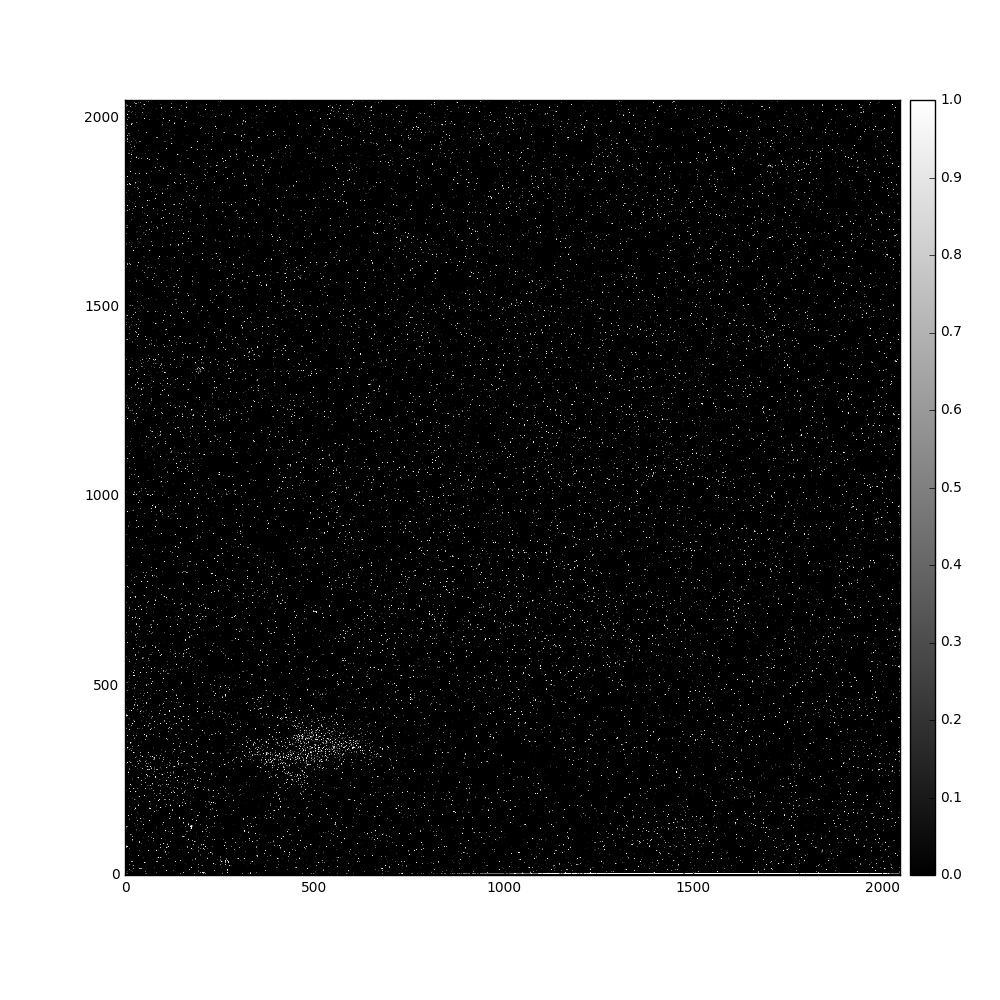
\includegraphics[width=1\linewidth]{badpixelmap}
  \caption{bad pixel map}
  %\label{fig:sub1}
\end{subfigure}\hfill
\begin{subfigure}{.48\textwidth}
  \centering
  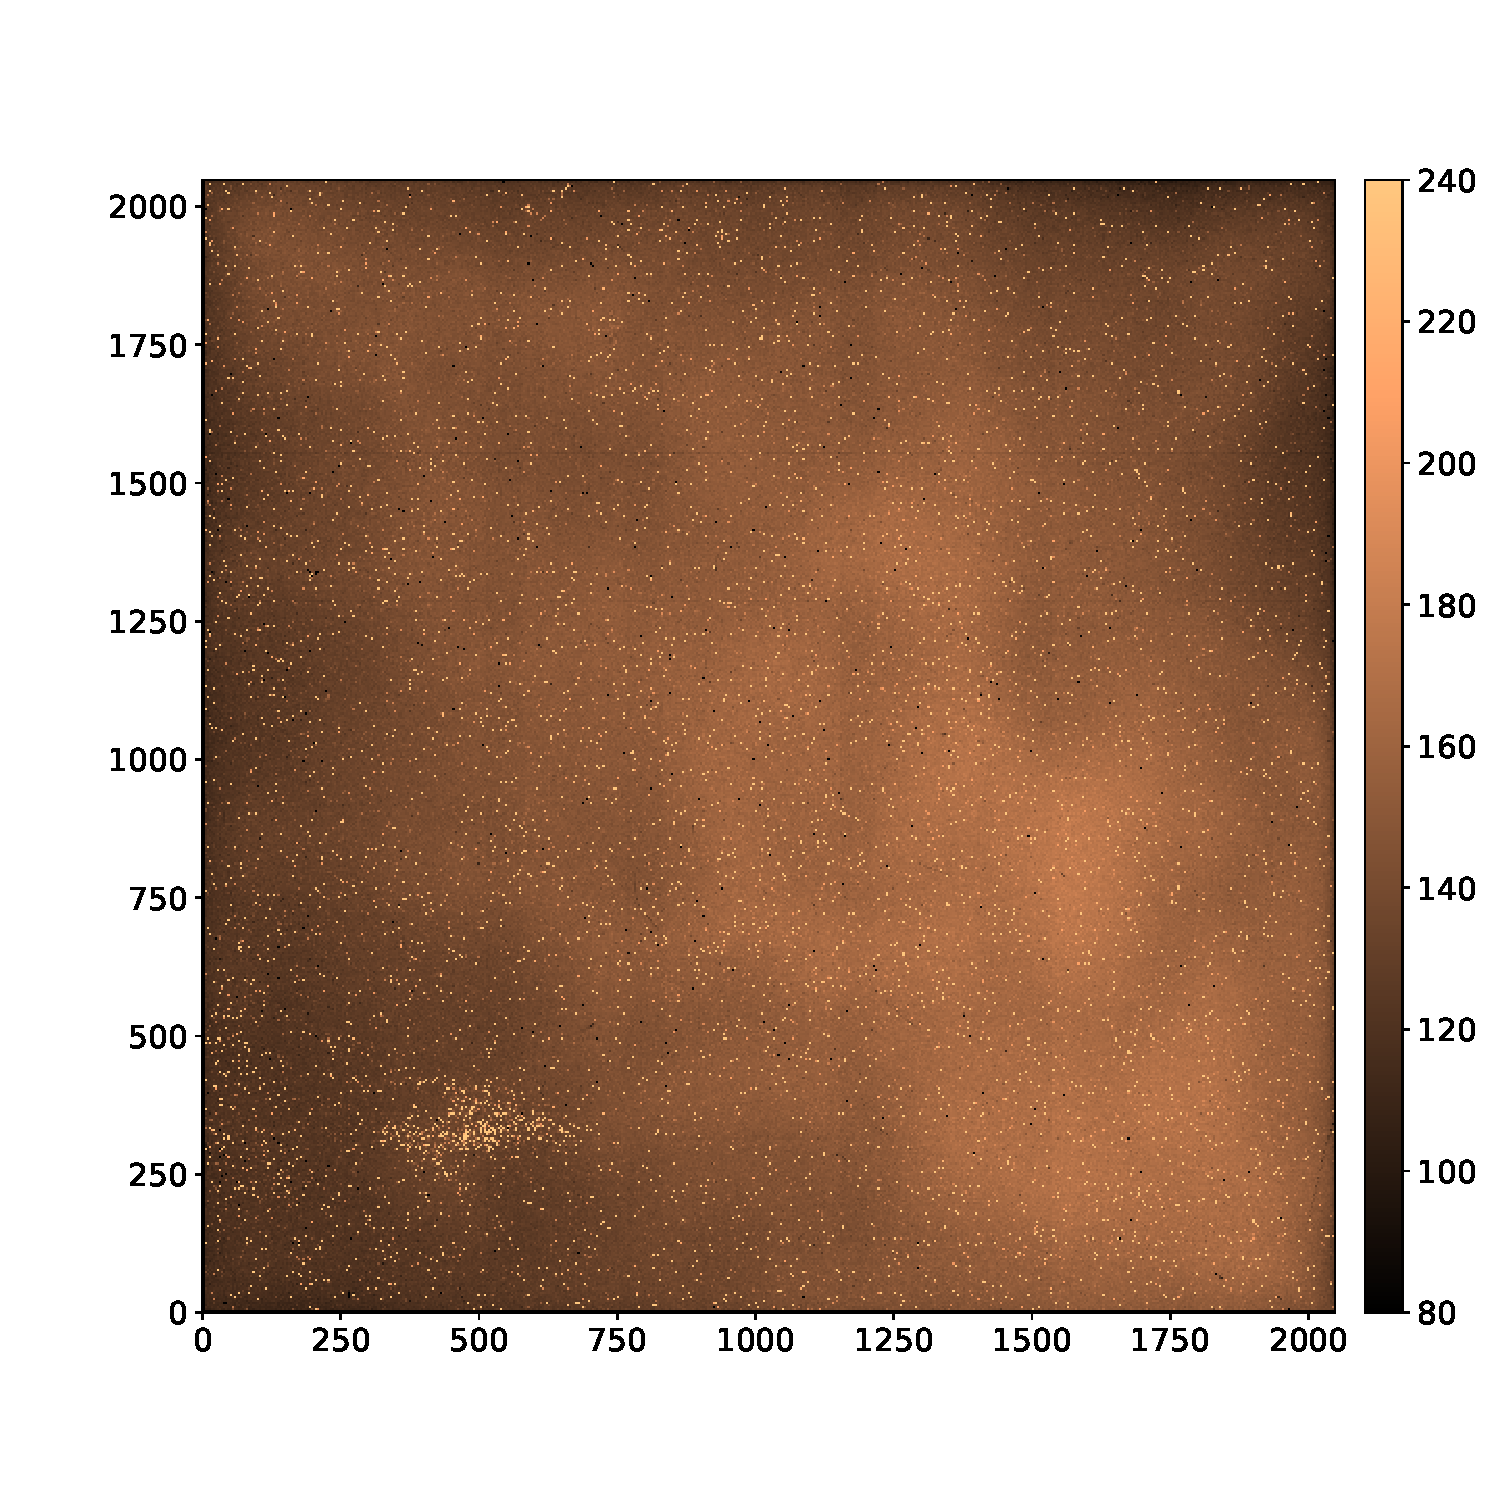
\includegraphics[width=1\linewidth]{dark}
  \caption{master dark}
  %\label{fig:sub2}
\end{subfigure}
\caption{result of the master dark recipe}
\label{fig:masterdark}
\end{figure}

\subsection{Detector flat}
\begin{figure}[!b]
\centering
\begin{subfigure}{.48\textwidth}
  \centering
  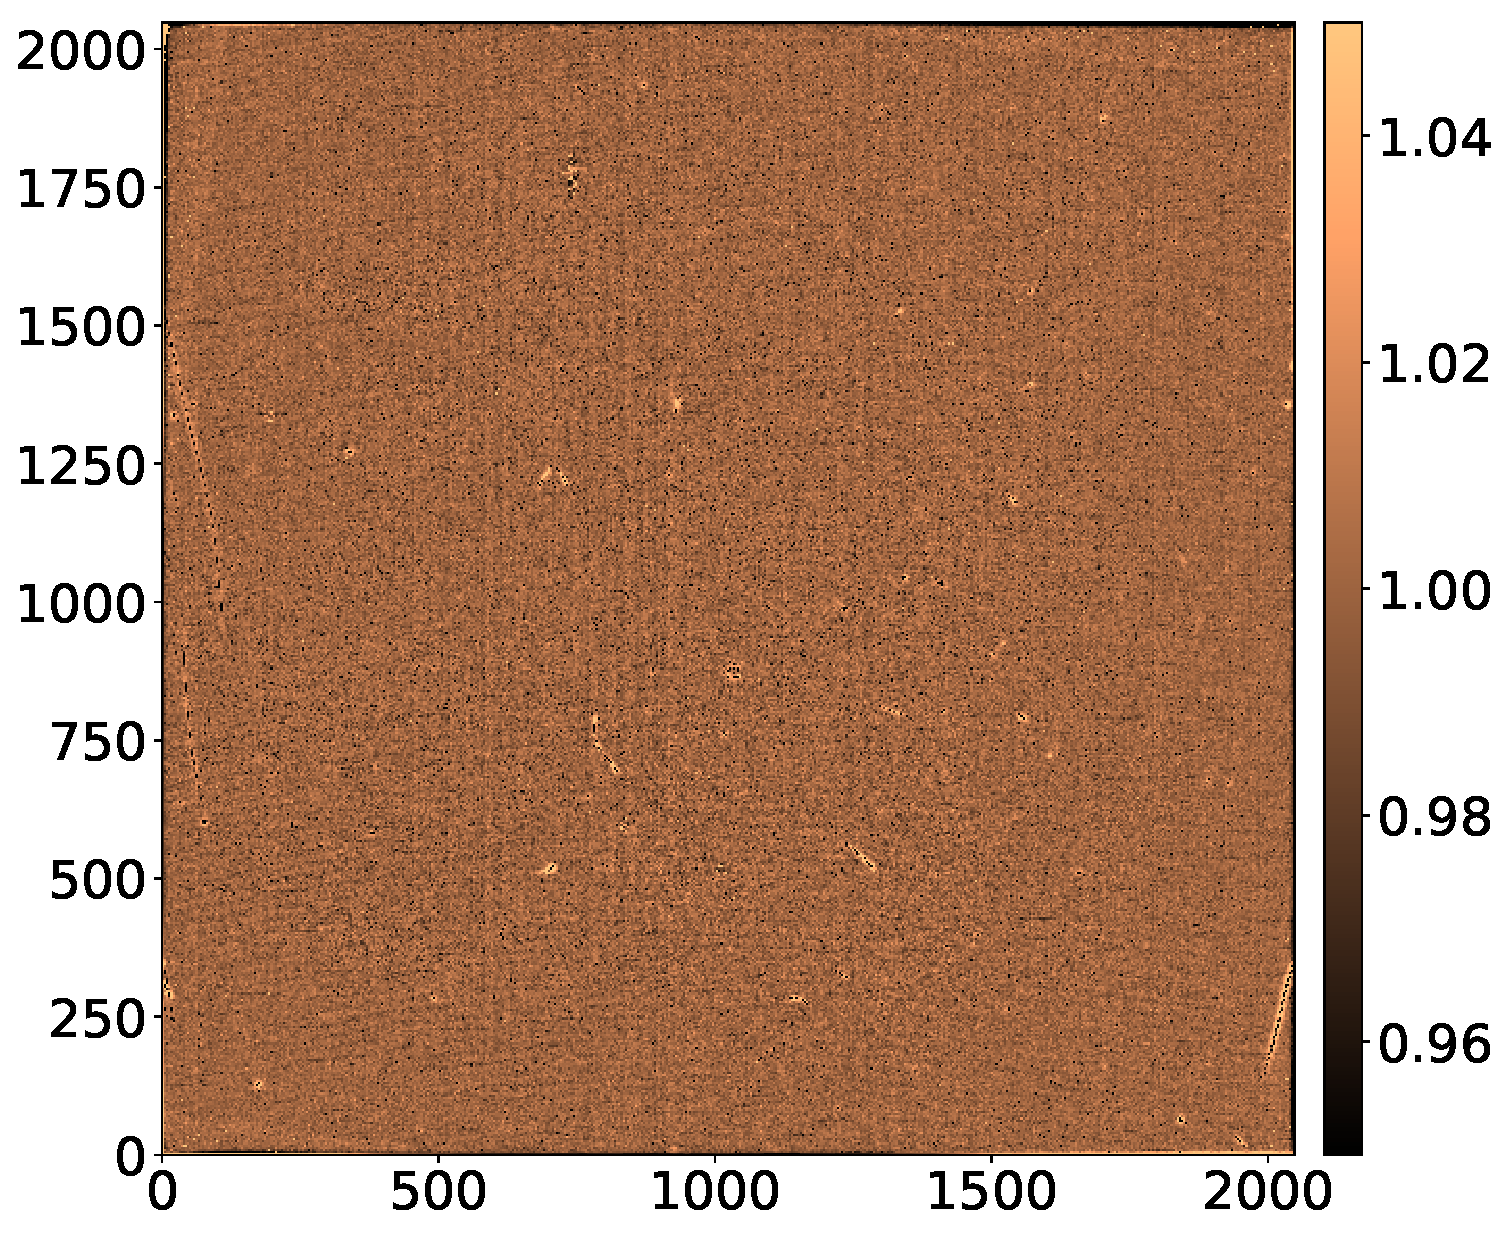
\includegraphics[width=1\linewidth]{masterdetectorflat}
  \caption{master detector flat}
  \label{fig:masterdetectorflat}
\end{subfigure}\hfill
\begin{subfigure}{.48\textwidth}
  \centering
  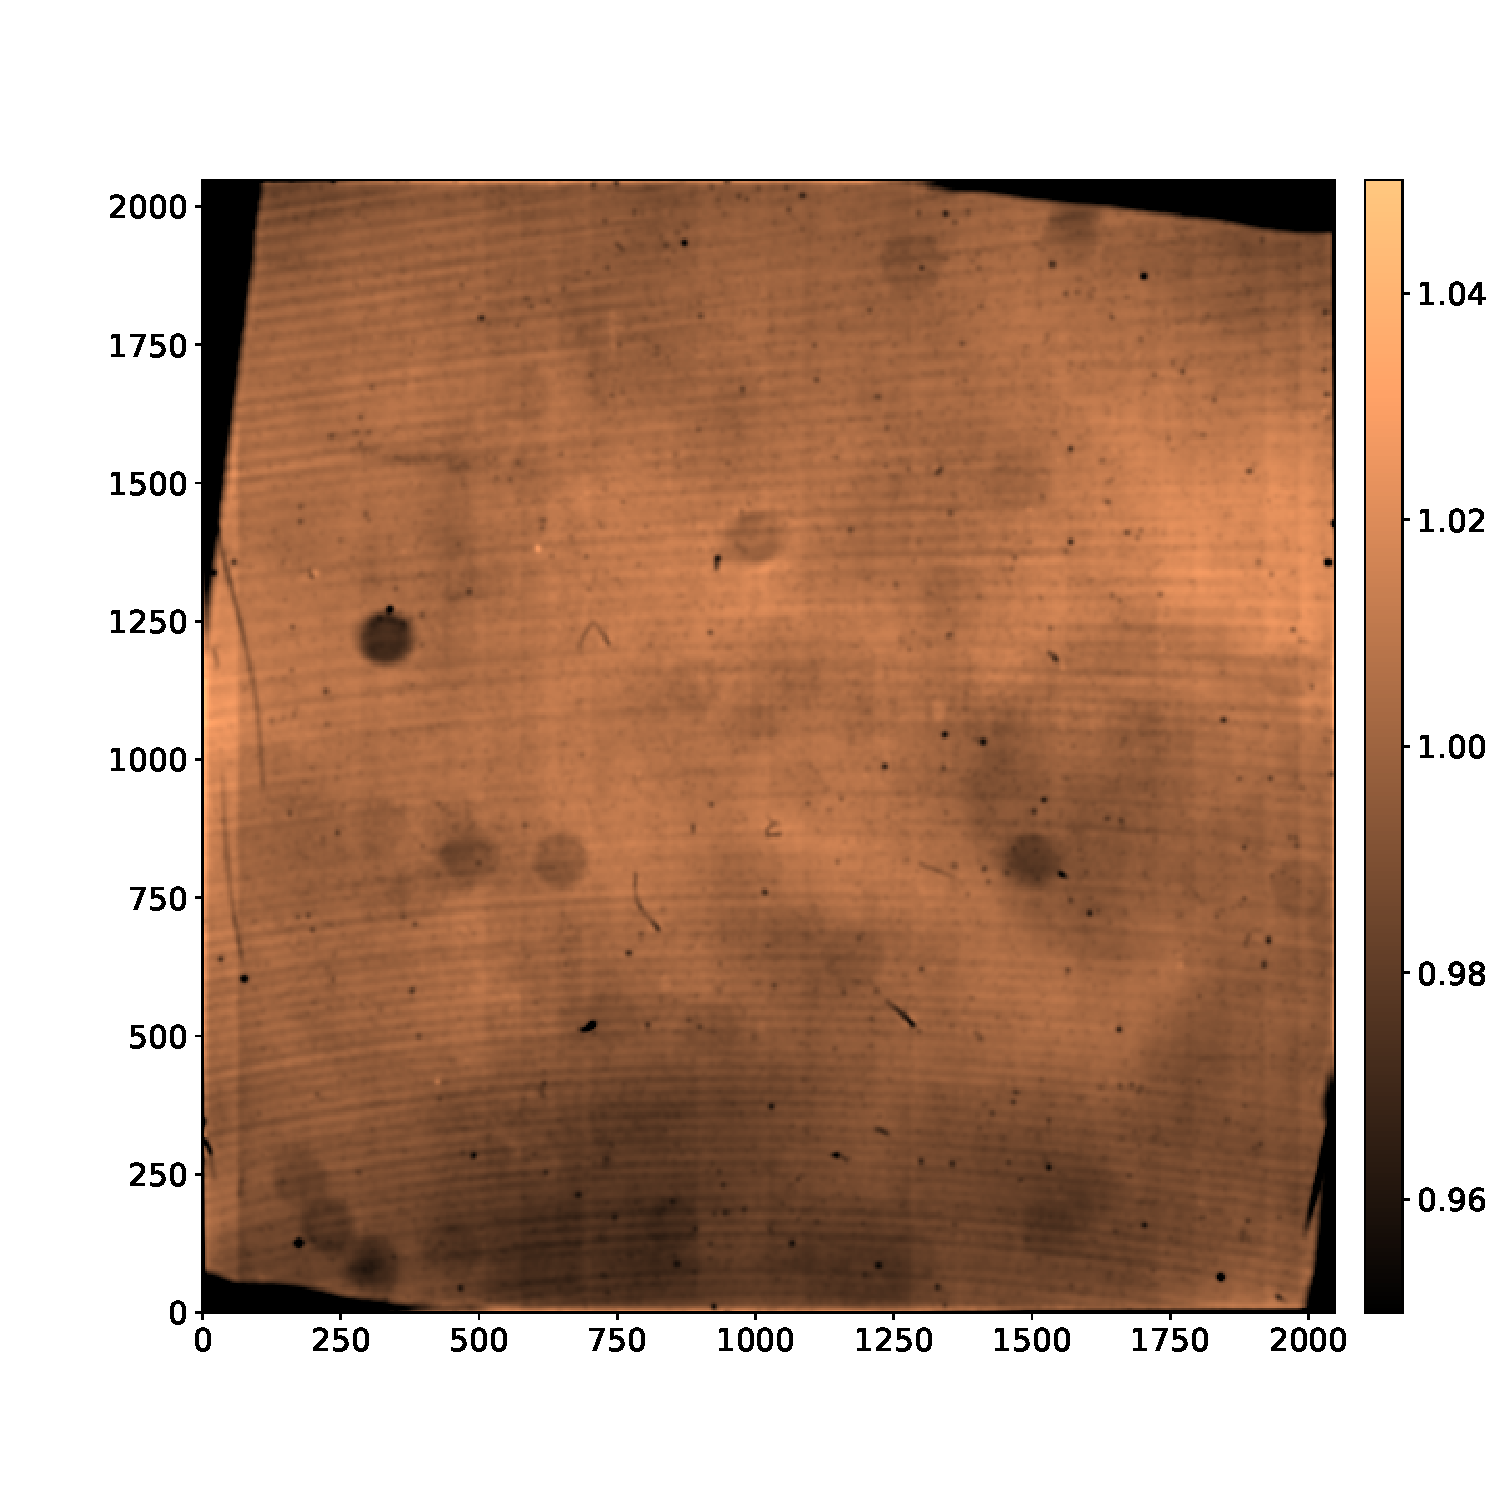
\includegraphics[width=1\linewidth]{largescaleflat}
  \caption{large scale flat}
  \label{fig:largescaleflat}
\end{subfigure}
\caption{result of the detector flat recipe}
%\label{fig:masterdark}
\end{figure}
At this step, the variation in sensitivity of the different pixels on the detector was measured. This can be done by using the extreme useful ability of the IFS to obtain flats with the shutter of the instrument closed and one of its internal calibration sources turned on. This means that the detector can be illuminated directly, which enabled us to correct for the distortions of the detector itself. The distortions in the optical path are measured in the recipe that produces the instrument flat, described in the next paragraph. 
\bigskip

Since the IFS uses a range of wavelengths, different detector flats are needed to calibrate all pixels properly. The recipe returns the combined master flat frames for the different lamps that are used. The best flat to use in the rest of the recipes are the master detector flats Figure \ref{fig:masterdetectorflat}. Large scale flats are master flat frames that are smoothed with a gaussian. On this images the large scale structures in pixel to pixel variation in the signal response of the detector get visible, such as ghosts. Large scale flats and pre-amplifier flats can be used as a calibration file for the actual detector flat recipe, but if they are not provided, they are created from the raw data. One of the large scale flats is illustrated in figure \ref{fig:largescaleflat}

\subsection{Instrument flat}
\begin{figure}[!b]
\centering
\begin{subfigure}{.48\textwidth}
  \centering
  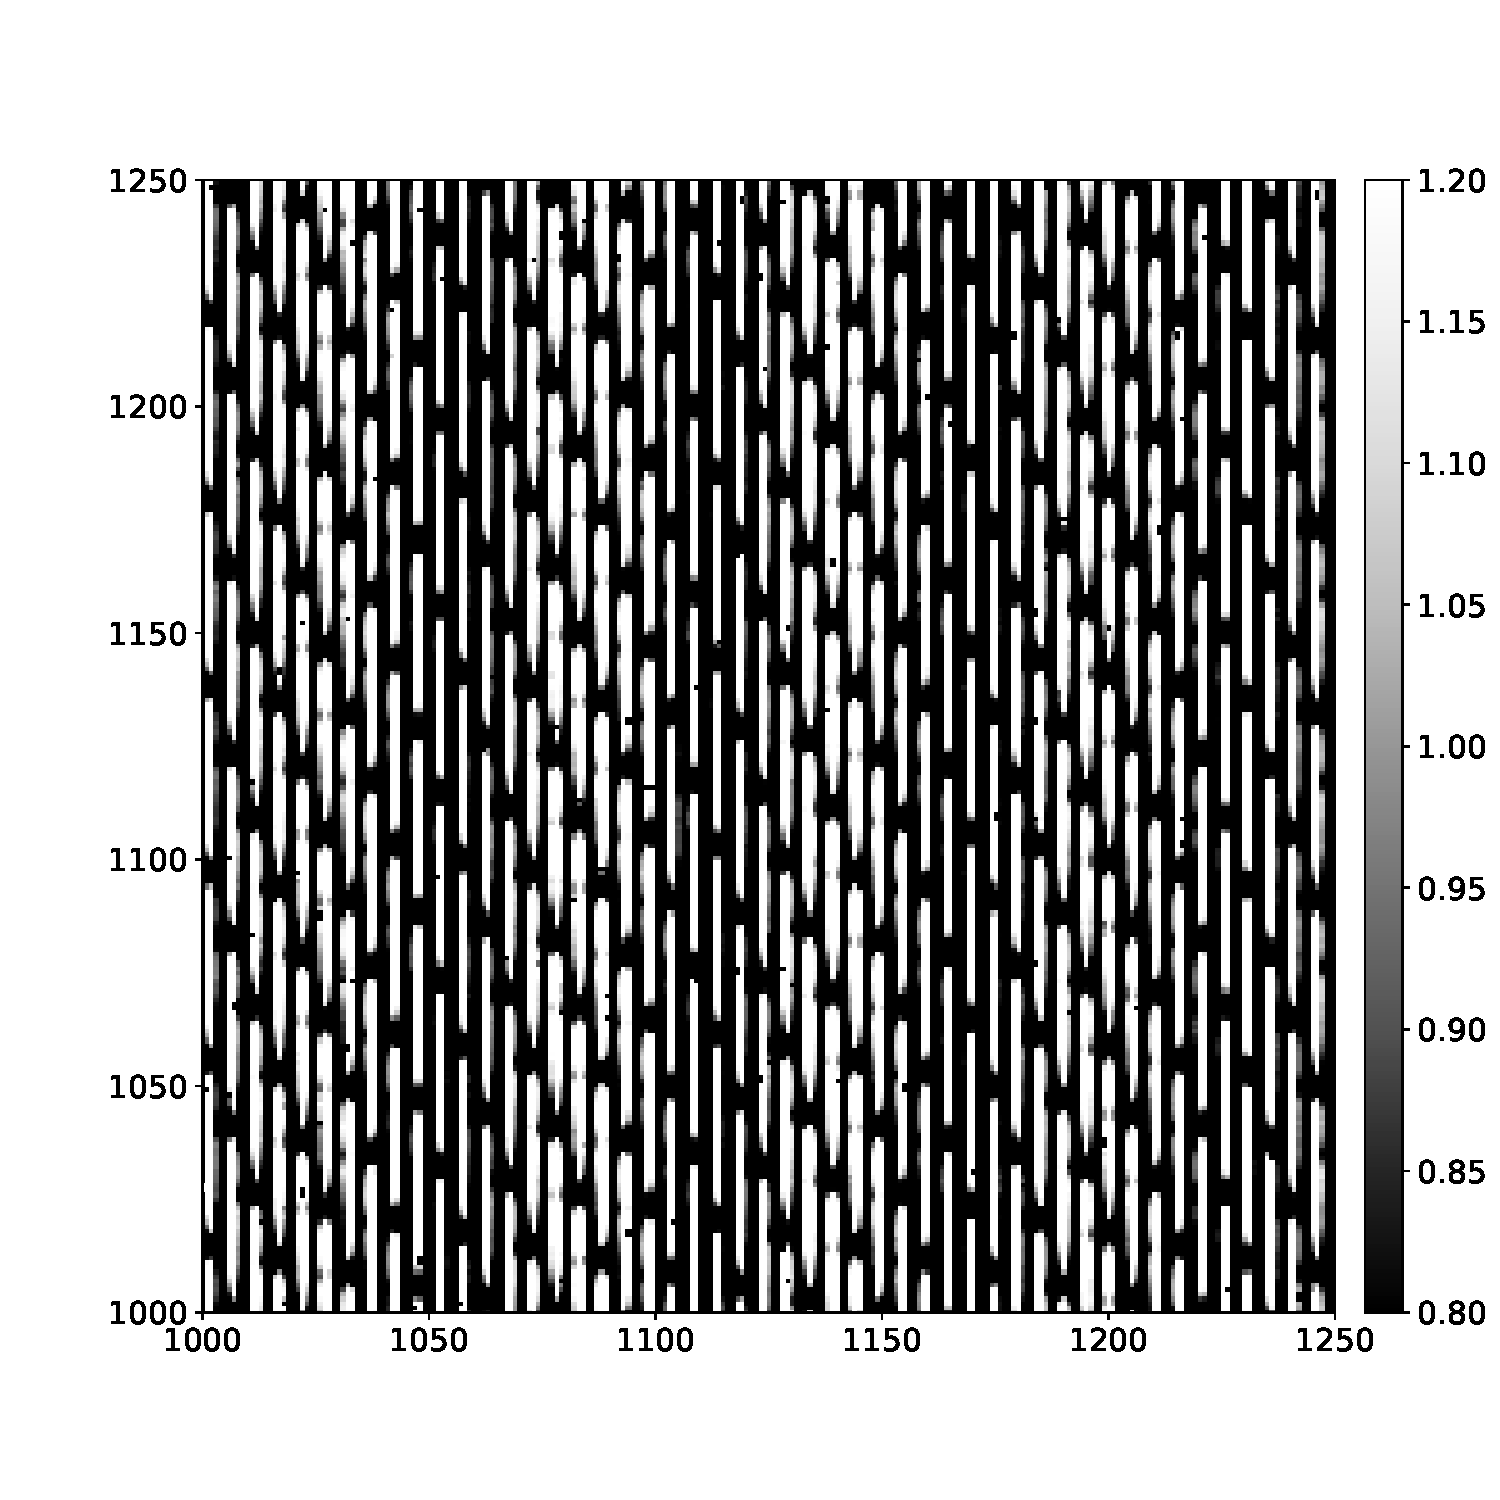
\includegraphics[width=1\linewidth]{instrumentflat}
  \caption{zoomed instrument flat}
  %\label{fig:preampflat}
\end{subfigure}\hfill
\begin{subfigure}{.48\textwidth}
  \centering
  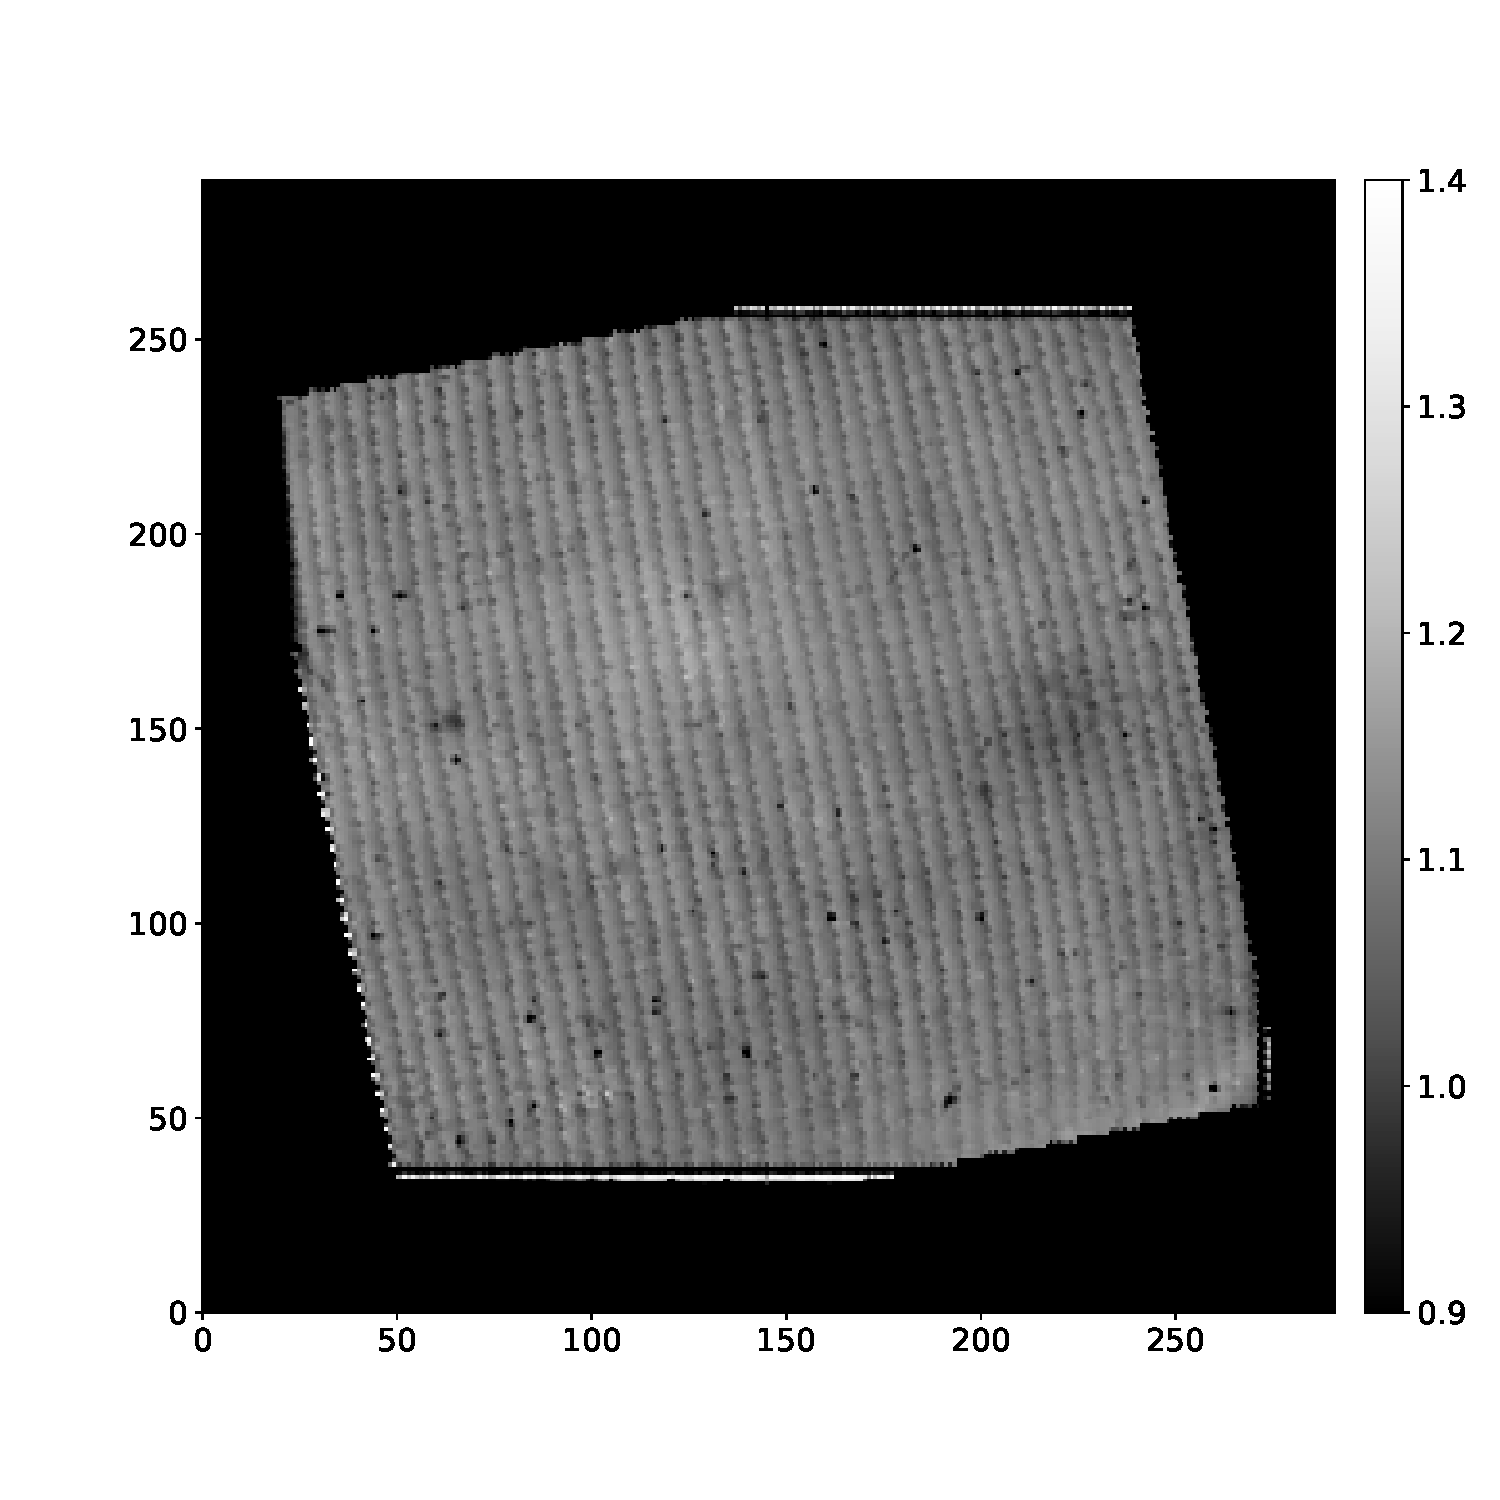
\includegraphics[width=1\linewidth]{IFU_flat}
  \caption{IFU flat}
  %\label{fig:largescaleflat}
\end{subfigure}
\caption{result of the instrument flat recipe}
\label{fig:instrumentflatrecipe}
\end{figure}
Instrument flats are obtained by taking a flat with three or four of the external calibration lamps on and is used to correct for the varying througput in the common path of the telescope and the instrument. After the dark subtraction, the flat field is divided by the detector flat. what has the effect of removing the detector response. This recipe returns both an instrument master flat which is the combined and reduced flat field before removing the detector response and the response of the integral field unit (IFU), which is the flat field after removing the detector response. The first can be used only for calibrating other calibration data, the latter can be used to reduce science data. The IFU flat field can be produced only if a reduced wavelength calibration is given. The production of the instrument flat is already possible with the positions of the spectrums only and is used to correct for the distortion of the lenslet grid in the wavelength calibration. The IFU flat does not give all pixels a sensitivity value, but assuming that most of the spatial distortion is due to the lenslet grid, the recipe returns the response of each individual lenslet. It gives for all pixels in the same spectrum a median value. This is why the IFU flat contains a typical stripe like feature. Both the IFU flat and the instrument flat are shown in figure \ref{fig:instrumentflatrecipe}. 

\subsection{Positioning spectra}
\begin{figure}[!b]
\centering
\begin{subfigure}{.48\textwidth}
  \centering
  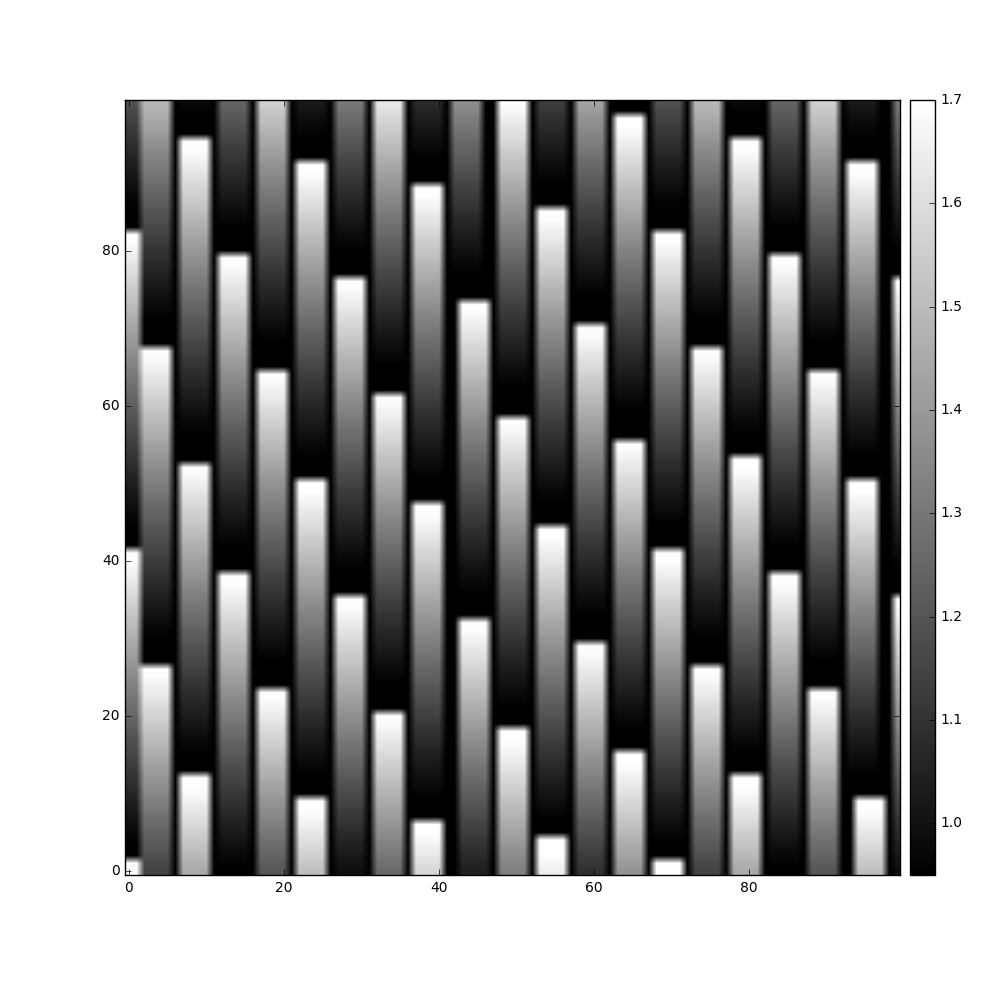
\includegraphics[width=1\linewidth]{specpos}
  \caption{zoomed positions of the spectra}
  \label{fig:specpos}
\end{subfigure}\hfill
\begin{subfigure}{.48\textwidth}
  \centering
  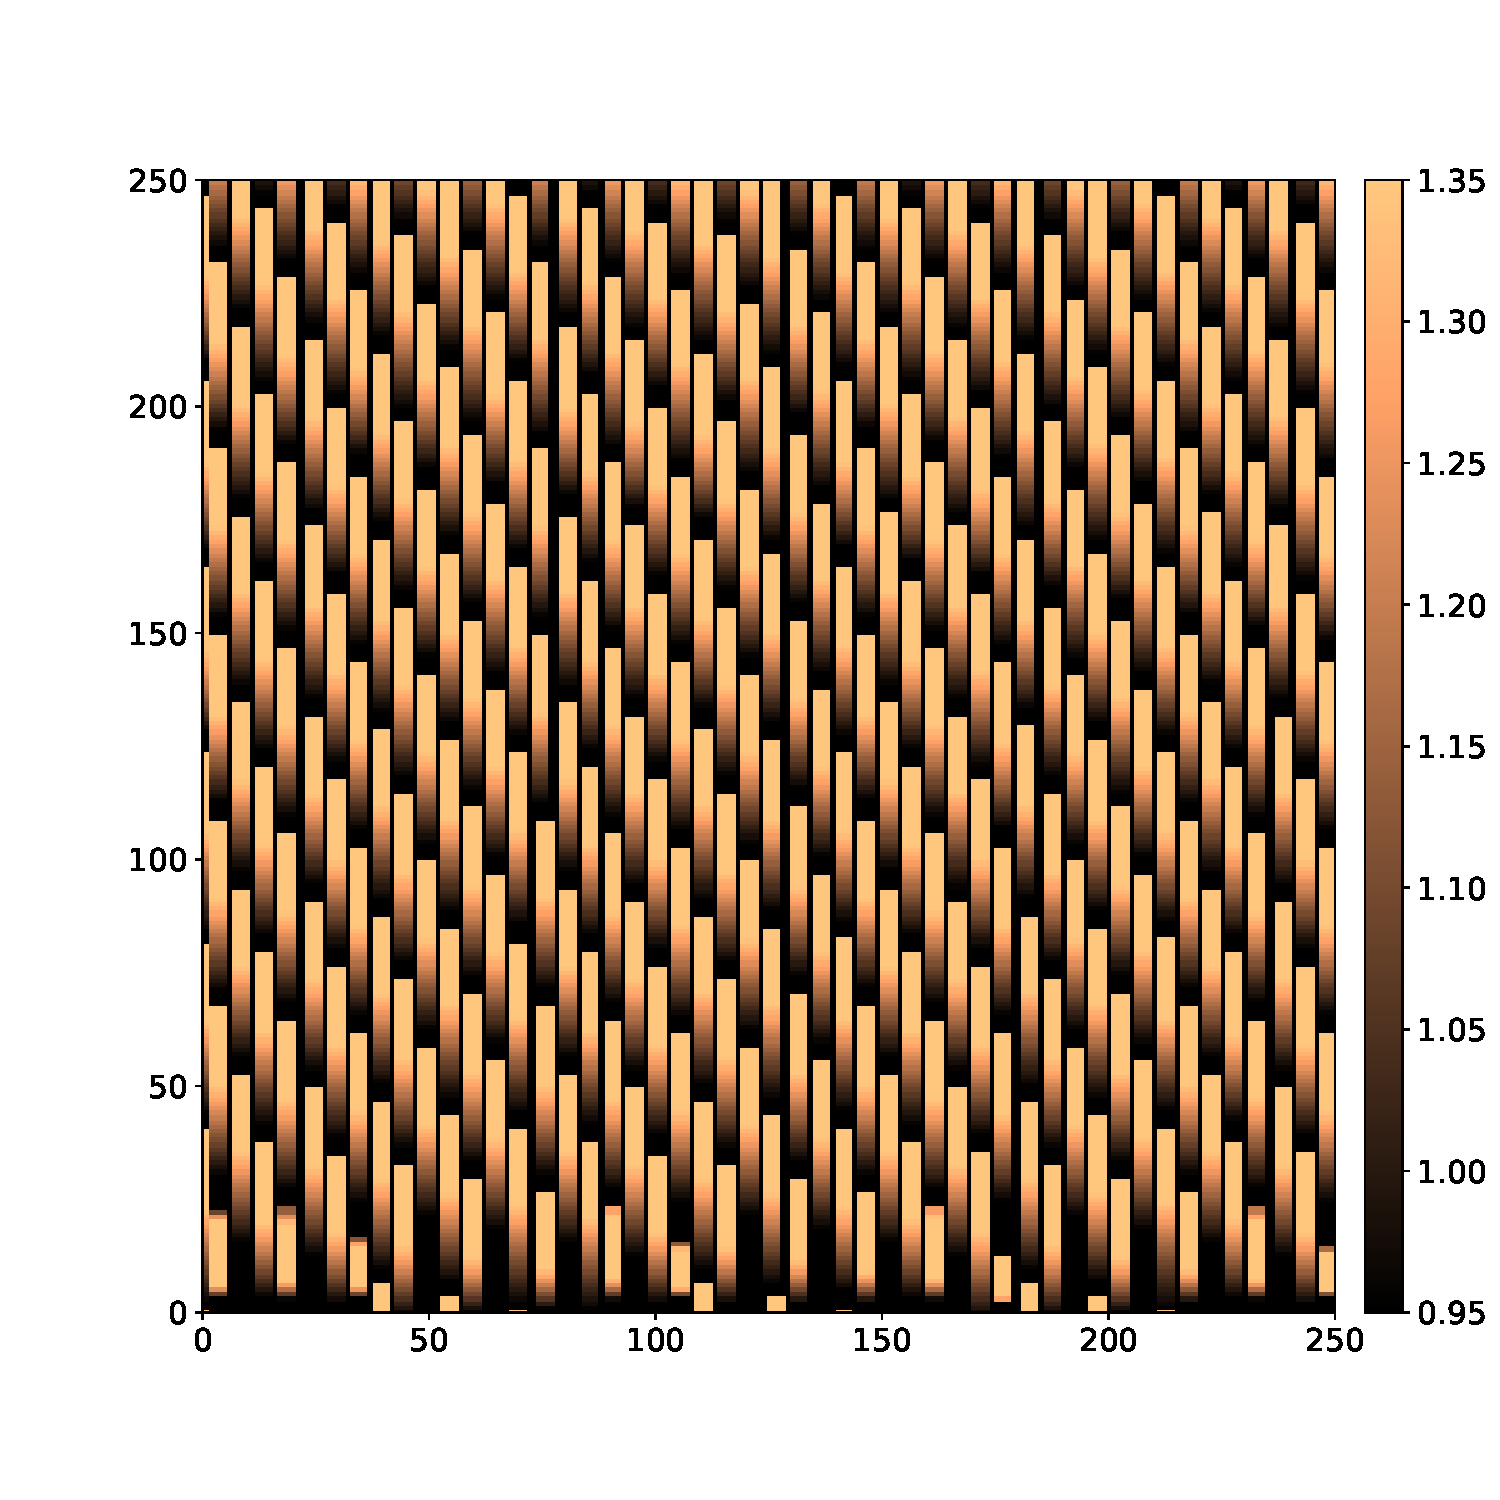
\includegraphics[width=1\linewidth]{wavecalib}
  \caption{zoomed wavelength calibration}
  \label{fig:wavecal}
\end{subfigure}
\caption{}
%\label{fig:masterdark}
\end{figure}

The spectra positioning recipe determines the exact position of the different spectra on the detector with an accuracy of about 4 $\mu m$, which corresponds to 0.2 pixels on the detector \citep{Desidera}. This is enough to build a map with the location of the spectra, associating each pixel to an individual lenslet. It associates pixels with wavelengths according to a lenslet model. Note that this is a non-linear model, as is visible in \ref{fig:specpos}. Each pixel in this image has the value of the corresponding wavelength in micron. This model is just a good guess, the exact wavelength can be obtained by running the wavelength calibration. The seperation between the positioning of the spectra and the wavelength calibration makes the positioning of the spectra much better, which is the reason why they have split these steps in two different recipes. The raw calibration data for the spectra positioning recipe is obtained by illuminating the instrument with an external white calibration light source that is uniformly scattered by use of an integrating sphere that diffuses the incoming light, but preserves the power. A zoomed piece of the spectra positioning image is shown in figure \ref{fig:specpos}

\subsection{Wavelength calibration}
The wavelength calibration recipe refines the wavelength of the different pixels, by using data that is obtained by illuminating the instrument with three or four external lasers, emitting at 0.9877, 1.1237, 1.3094 and 1.5451($\mu m$). These lasers have been uniformly scattered with the same integrating sphere as mentioned in the section about the spectra positioning. The recipe tries to fit a spectrum on the positions that are determined in the spectra positioning recipe. Note that if a part of the spectrum does not fit on the detector, the recipe is unable to fit a spectrum, which is illustrated in figure \ref{fig:wavecal}.

\subsection{Science reduction}
In the science reduction recipe the science frames are finally calibrated. This recipe needs all the output of the different calibration recipes as input alongside the raw science frames in order to correct properly for all the aberations. This recipe uses all the reduced calibration data in order to correct the data for all the different noise sources and asign pixels of the detector to pixels of the result in the end: a 39 x 291 x 291 datacube.

\section{Post-processing methods}
After the basic science reduction, the disk around the star is still not visible to the naked eye. Post processing techniques, based on subtracting a model of the stellar PSF were needed to gain the best result in detection of the disk. Two different methods are used to make a model for the stellar PSF: angular differential imaging (ADI) and spectral differential imaging (SDI). But before constructing a model for the PSF, the data needs to be centered correctly.

\subsection{Centering}
The telescope is calibrated such that the star is about in the center of the image, but there is always a slight offset. Center frames can be used to determine the center of the images on a level up to tenths of a pixel. These center frames are science frames containing also four artificial satellite spots, created by the adaptive optics system with the center of the star exactly in the middle of the four satellite spots, Figure \ref{fig:centerframe}. These center frames are usually taken before, during and after the science run, such that for small changes of the position of the center in the dataset can be corrected.
\begin{figure}[!t]
\centering
\begin{subfigure}{.48\textwidth}
  \centering
  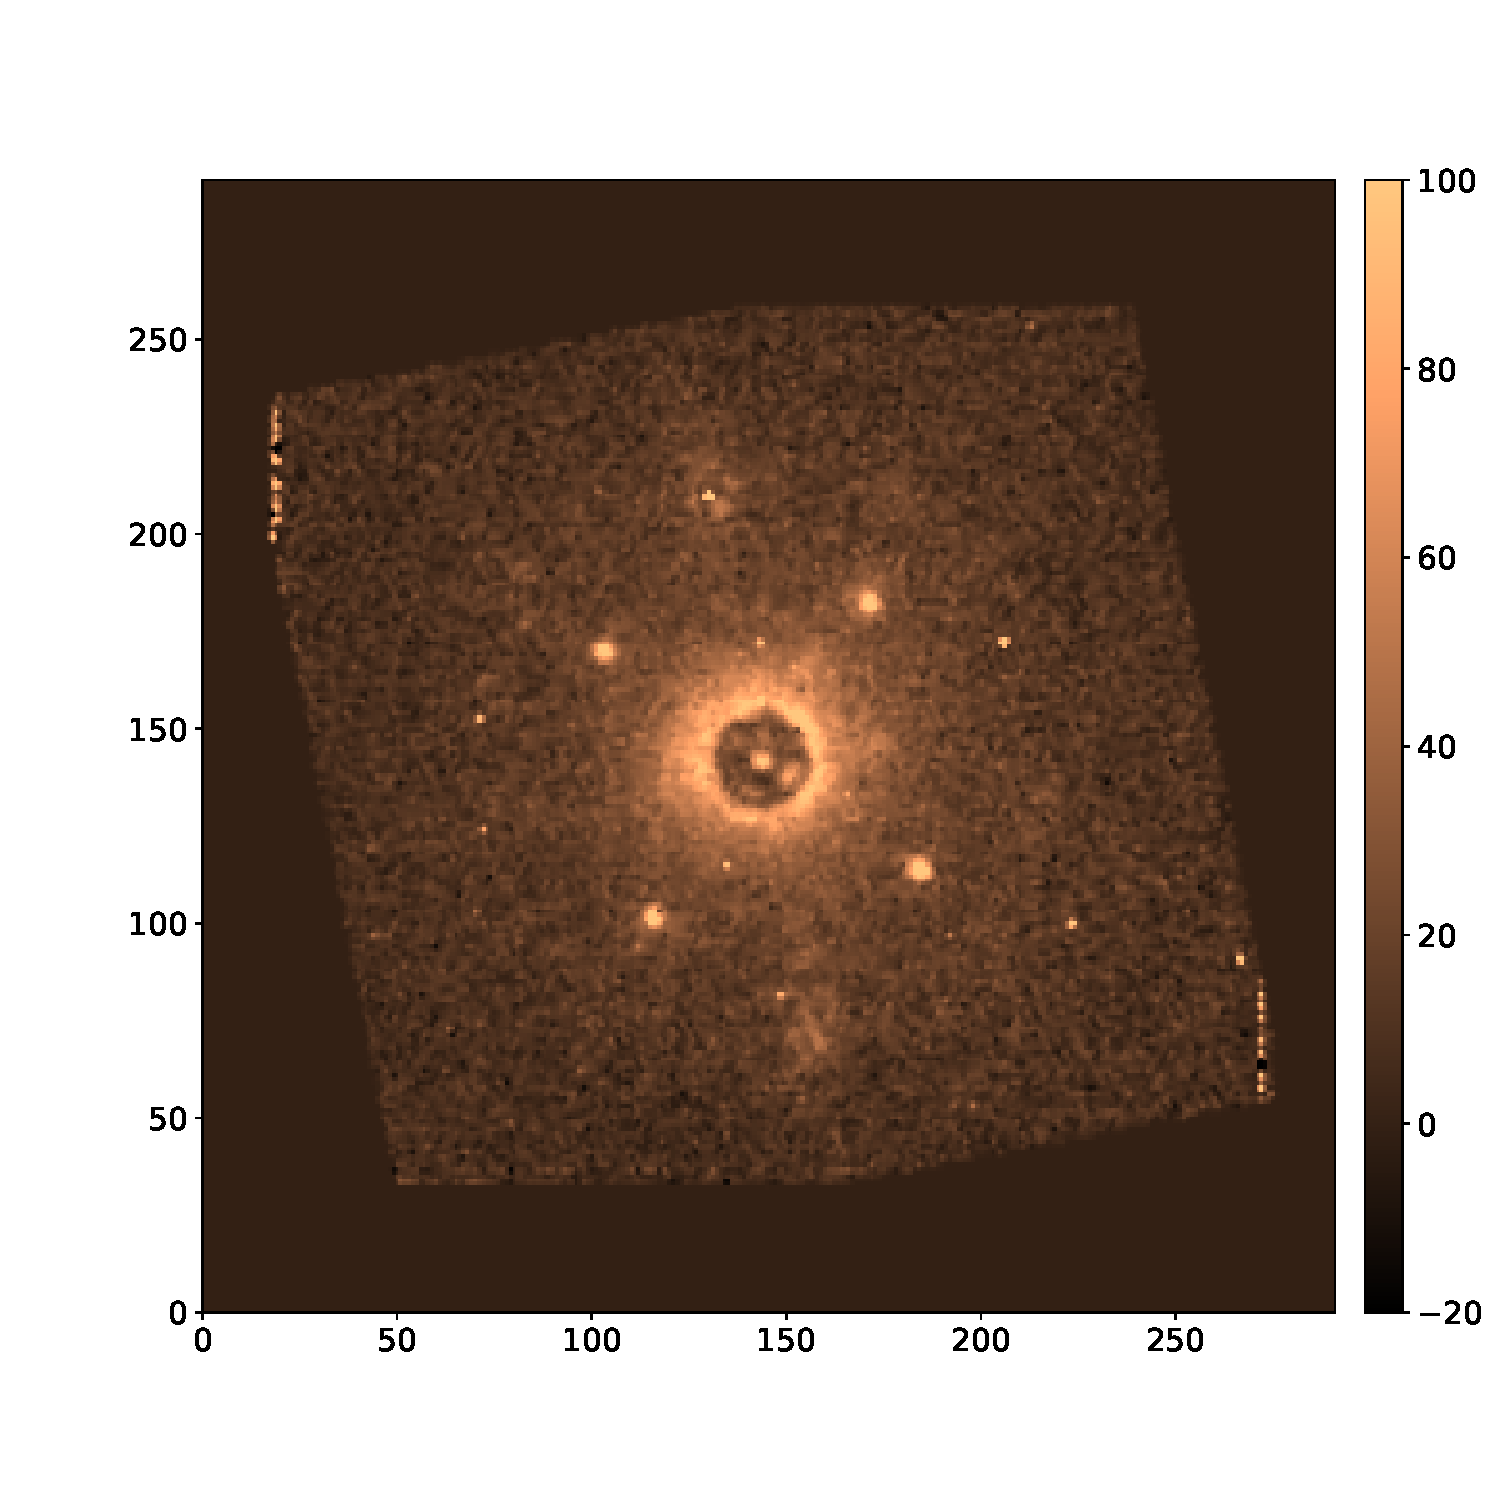
\includegraphics[width=1\linewidth]{centerframe}
  \caption{one of the 39 wavelength slices of a reduced center exposure\\}
  \label{fig:centerframe}
\end{subfigure}\hfill
\begin{subfigure}{.48\textwidth}
  \centering
  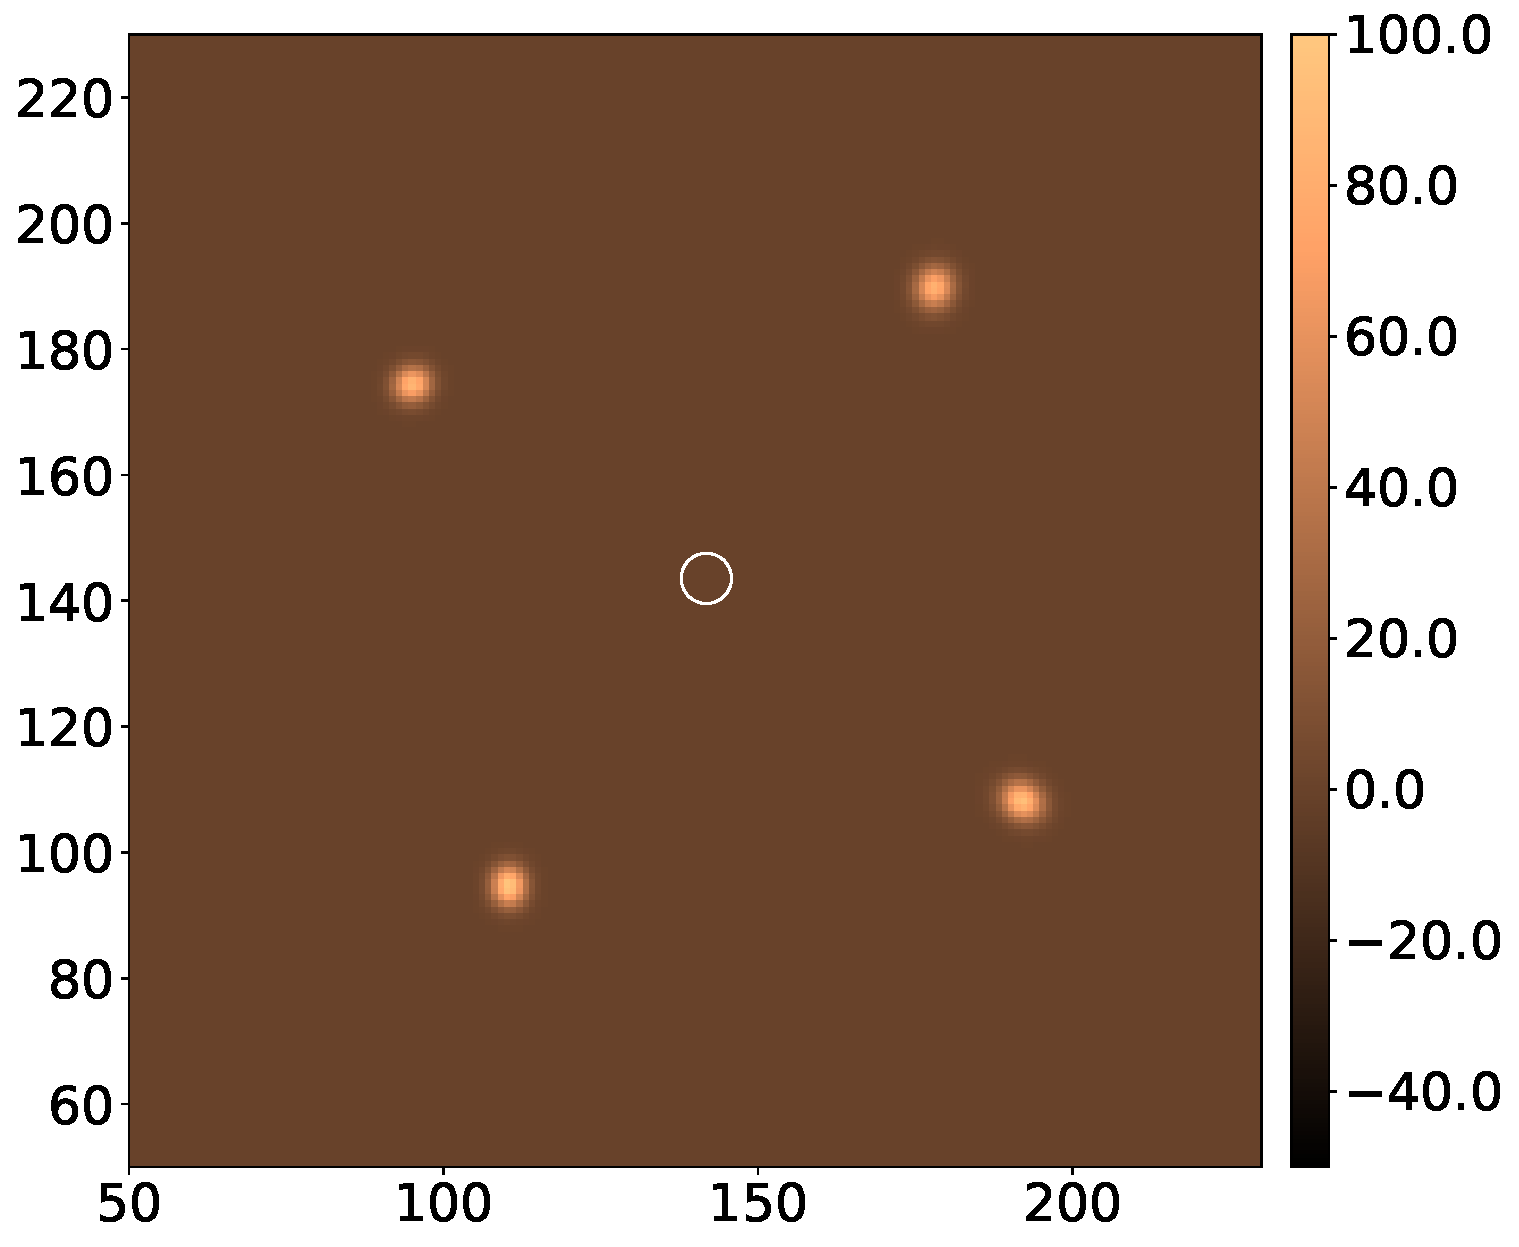
\includegraphics[width=1\linewidth]{centermodel}%
  \caption{model of the four satellite spots with the center of the star marked with a white circle}
  \label{fig:centermodel}
\end{subfigure}
\caption{results of the centering routine: four gaussians are fitted over the satellite spots in order to determine the exact position of the center of the frame.}
%\label{fig:masterdark}
\end{figure}

\begin{figure}[!b]
\centering 
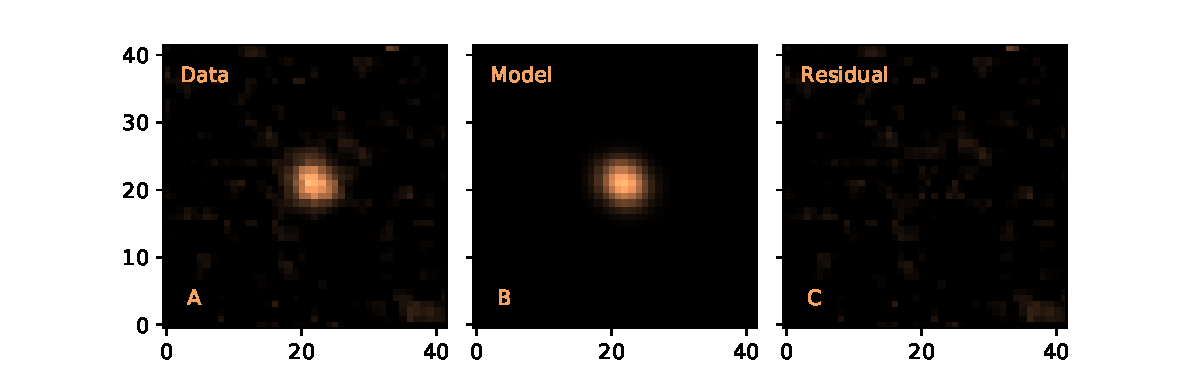
\includegraphics[width = \textwidth]{resultmodel}
\caption{\textbf{A:} one of the raw satellite spots, \textbf{B:} model of the satellite spot,\\ \textbf{C:} residual after subtracting the model of the data} 
\label{fig:resultmodel}
\end{figure}
\bigskip
Center frames are reduced in the same way as normal science frames, using the same dark and flat frames. Then the image is first smoothed with a gaussian with a standard deviation of 25 that filters all the high frequency noise out and leaves a clean image of the four satellite spots. After that a single gaussian is fitted over each of the four satellite spots and a model is created for the combined satellite spots. The position of the center can be determined from the positions of the fitted gaussians. The fit of all the satellite spots on the centerframes were good, leaving almost no residual signal after subtracting the model from the data, as illustrated in Figure \ref{fig:resultmodel}. The positions of the satellite spots are accurately measured with an uncertainty between 0.40 and 0.45 pixels for both the x and y co\"ordinate for each spot. The uncertainty on the coordinates of the center is hence 0.2 pixels.

\subsection{Angular differential imaging}

\begin{wrapfigure}{R}{0.6\textwidth}
\centering
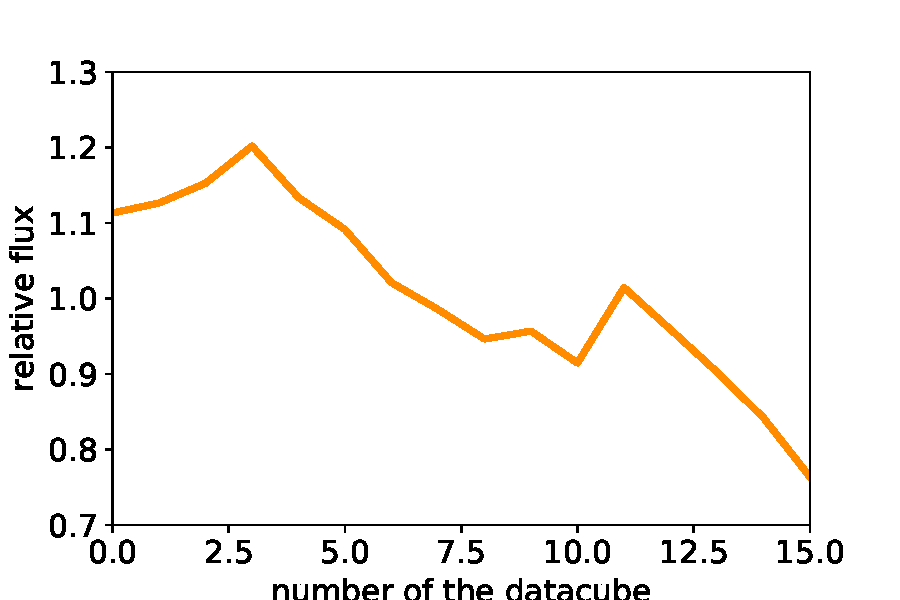
\includegraphics[width = 0.56\textwidth]{aonorm}
\caption{Relative flux of the different datacubes over time. This is used to normalize the data between different exposures.}
\label{fig:aonorm}
\end{wrapfigure}

ADI is a post-processing method that constructs a model for the stellar PSF out of the rotation of the field during the night \cite{Marois2005}. Normally, telescopes correct for the rotation of the earth and hence the rotation of the object on the detector. To apply ADI on data, this correction is switched off, such that the field rotates over time during the night. The star can be considered as a point source that does not change under rotation. The disk however, is rotational assymetric. The total field rotation during the observation run was 69 degrees, in 16 different exposures, meaning that the signal has changed a lot on the detector over time. Taking the median per pixel, per wavelength over the whole time should hence give a model for the PSF of the star. Subtracting this model from each individual frame and realigning the data with each other by rotating each frame with the known parallactic angle, gave good results. 
\bigskip

Since the data was taken with more than an hour between the first and last exposure, the flux of the object on the detector changes. This is partially due to changes in the sky during the night, but more due to changes in the quality of the correction of the adaptive optics during the night. To correct for this the median amount of flux in an annulus that grows in size with wavelength is measured. This annulus has an inner radius that is in each frame located just outside the outer ring of flux that is created by the coronograph. Since the PSF scales with $ \propto\lambda/D$, the radii of the annulus has to change for different wavelengths, to measure the flux in the same region of the PSF. The measured flux over wavelength is illustrated in Figure \ref{fig:aonorm}. With this relative flux the PSF of the star in different exposures can be normalized such that it is correctly subtracted in each frame in the procedure. After the subtraction and before combination of the different frames, the normalization is reversed, such that the signal is not amplified in certain frames.


\subsection{Spectral differential imaging}
\begin{wrapfigure}{R}{0.6\textwidth}
\centering
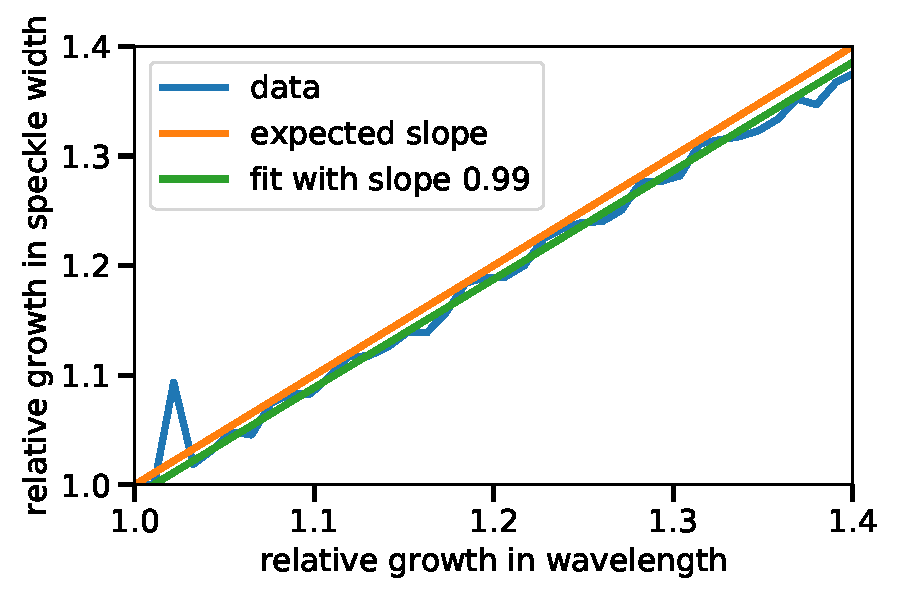
\includegraphics[width = 0.57\textwidth]{specklegrowth}
\caption{Relative growth in the size of the PSF of the star versus wavelength. Note data the data follows almost exactly the expected slope.}
\label{fig:specklegrowth}
\end{wrapfigure}
Spectral differential imaging is a post-processing method that constructs a model for the PSF of the star by use of the wavelength dependency of the PSF. The PSF of a star scales with $ \propto\lambda/D$, which means that the resolution and hence the scale of the PSF is directly proportional to the wavelength. We expect therefore that the PSF of the star increases linearly with wavelength. The signal of the disk however does not. This means that this should leave us with a model for the PSF after taking a median over all 39 spectral channels that does not contain anything of the disk signal. After subtracting this model from the data we scaled everything back to the original dimensions, such that the signal of the disk lines up in each spectral channel. The different exposures have been combined by rotating them with the corresponding parallactic angle after which a median for each pixel in each spectral channel over the different exposures is taken. This provided an image with the highest signal-to-noise ratio.
\bigskip

In order to check if the scale of the PSF is directly proportional to the wavelength, we measured the distance between the different artificially created satellite spots in the center image, using the same model as in the procedure that centers the science frames. The result of this measurement and the expected slope are plotted in Figure \ref{fig:specklegrowth}. This result indicates that the size of the PSF is indeed directly proportional to the wavelength, which means that the througput of the instrument does not spatially distort different wavelengths and that the wavelength calibration and positioning of the spectra is done in the right way.
\bigskip

\begin{wrapfigure}{R}{0.6\textwidth}
\centering
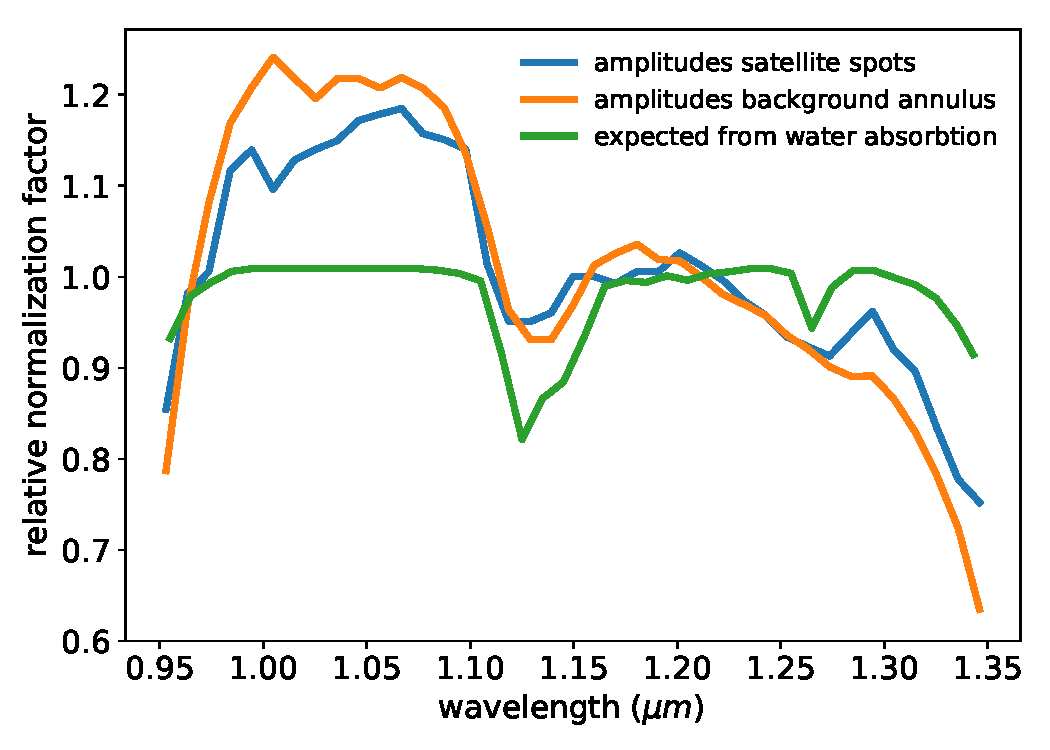
\includegraphics[width = 0.57\textwidth]{allnormalization}
\caption{The normalization factors used to normalize the data between different spectral channels. In green the expected correction due to water absorption in the atmosphere.}
\label{fig:throughputnorm}
\end{wrapfigure}

\noindent
Just as in the angular differential imaging, the data needs to be normalized before we take the median in order to get a good model of the PSF in each spectral channel. Since the throughput of the atmosphere, the instrument and the common path of the telescope is wavelength dependent, we had to normalize the flux in the different spectral channels. Our first try was to average the amplitude of the four fitted gaussians over the satellite spots in the center frames, but this did not turn out that well. Secondly we tried to measure the flux in a fixed annulus around the center, after scaling the different spectral channels such that the PSFs lined up, Figure \ref{fig:throughputnorm}.
\bigskip

The normalization factor as derived in the second way mentioned differed just a little from the one using the center frames, but this left us with good results in the end. The dips in the normalization factors line up with the expected dips in the throughput of the atmosphere due to absorbtion, Figure \ref{fig:throughputnorm}, since there is a big abundance of strong absorbtion lines of water in that part of the spectrum. The general trend is a decreasing flux over wavelength. The SED of the star peaks in the H band, as discussed in section 2.2 and illustrated in Figure \ref{fig:SED} \citep{Padgett}. This would indicate that the total incoming flux of the star should slighty increase over the range of the IFS. The fact that we see a decrease in flux instead is definitely due to wavelength dependencies in the throughput of the instrument as illustrated in Figure \ref{fig:systemthrougput}. 

\chapter{Results of post-processing methods}
\section{ADI}
\begin{figure}[!b]
\centering
\begin{subfigure}{.48\textwidth}
  \centering
  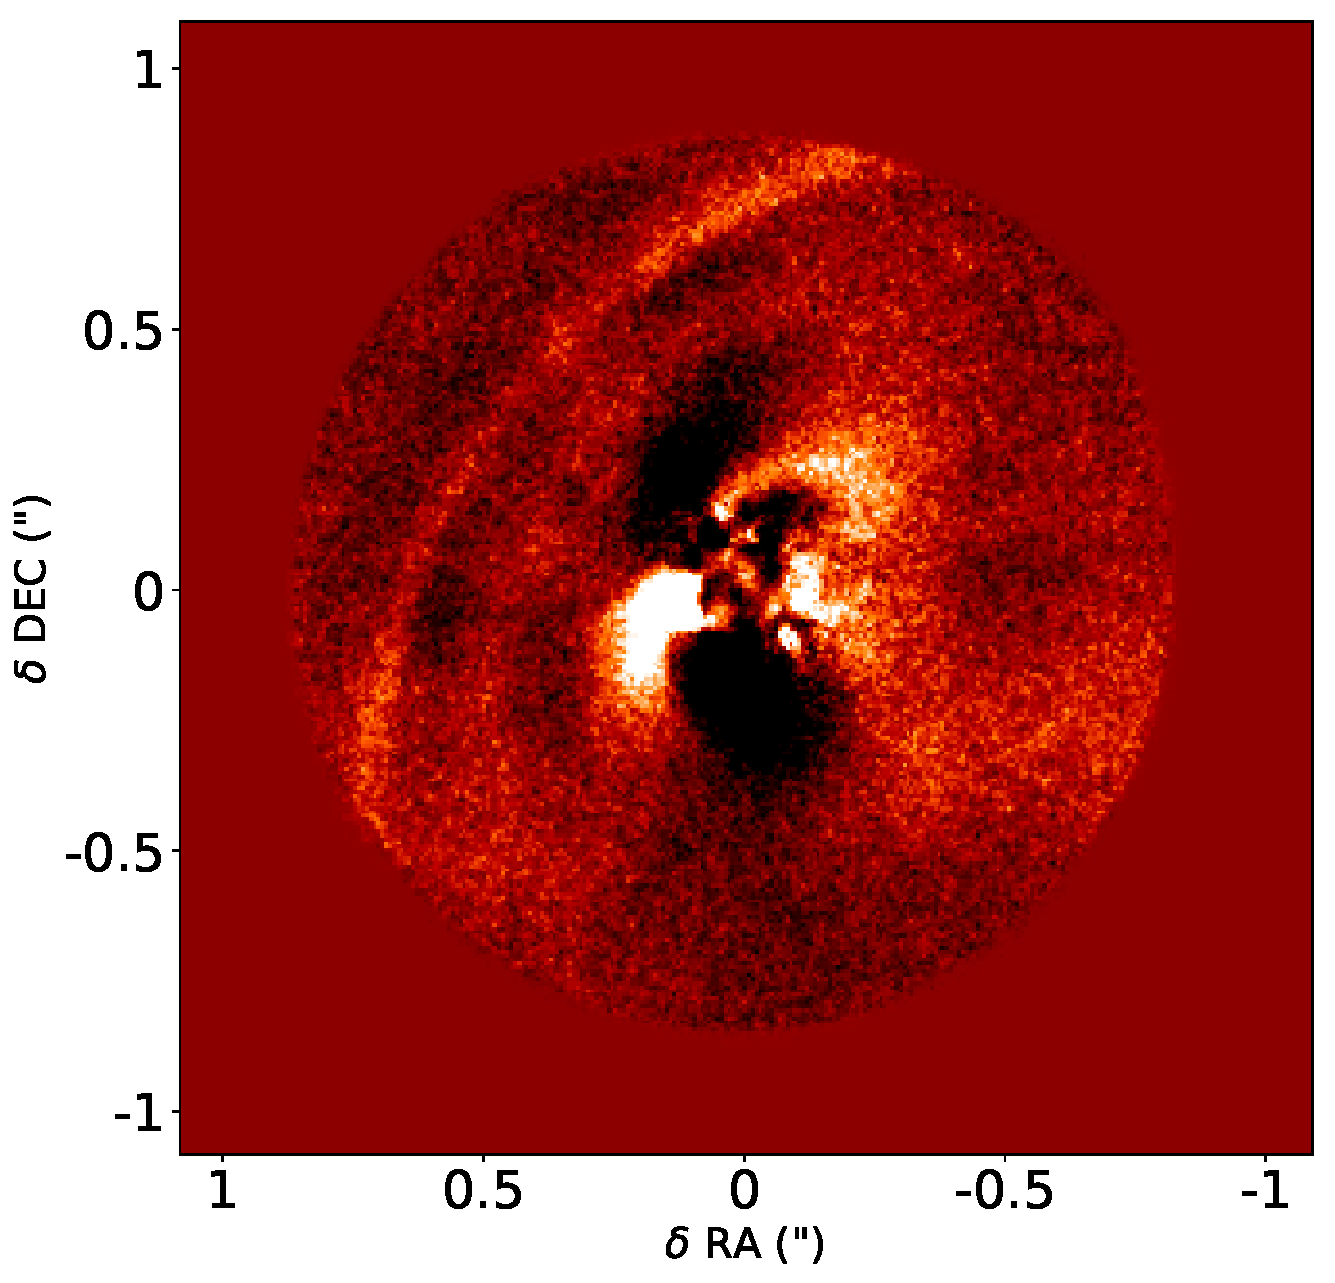
\includegraphics[width=0.8\linewidth]{ADI_tot}
  \caption{The median ADI image of all exposures over the whole Y-J wavelength range of RX J1615\\\\\\\\}
  \label{fig:ADItot}
\end{subfigure}\hfill
\begin{subfigure}{.48\textwidth}
  \centering
  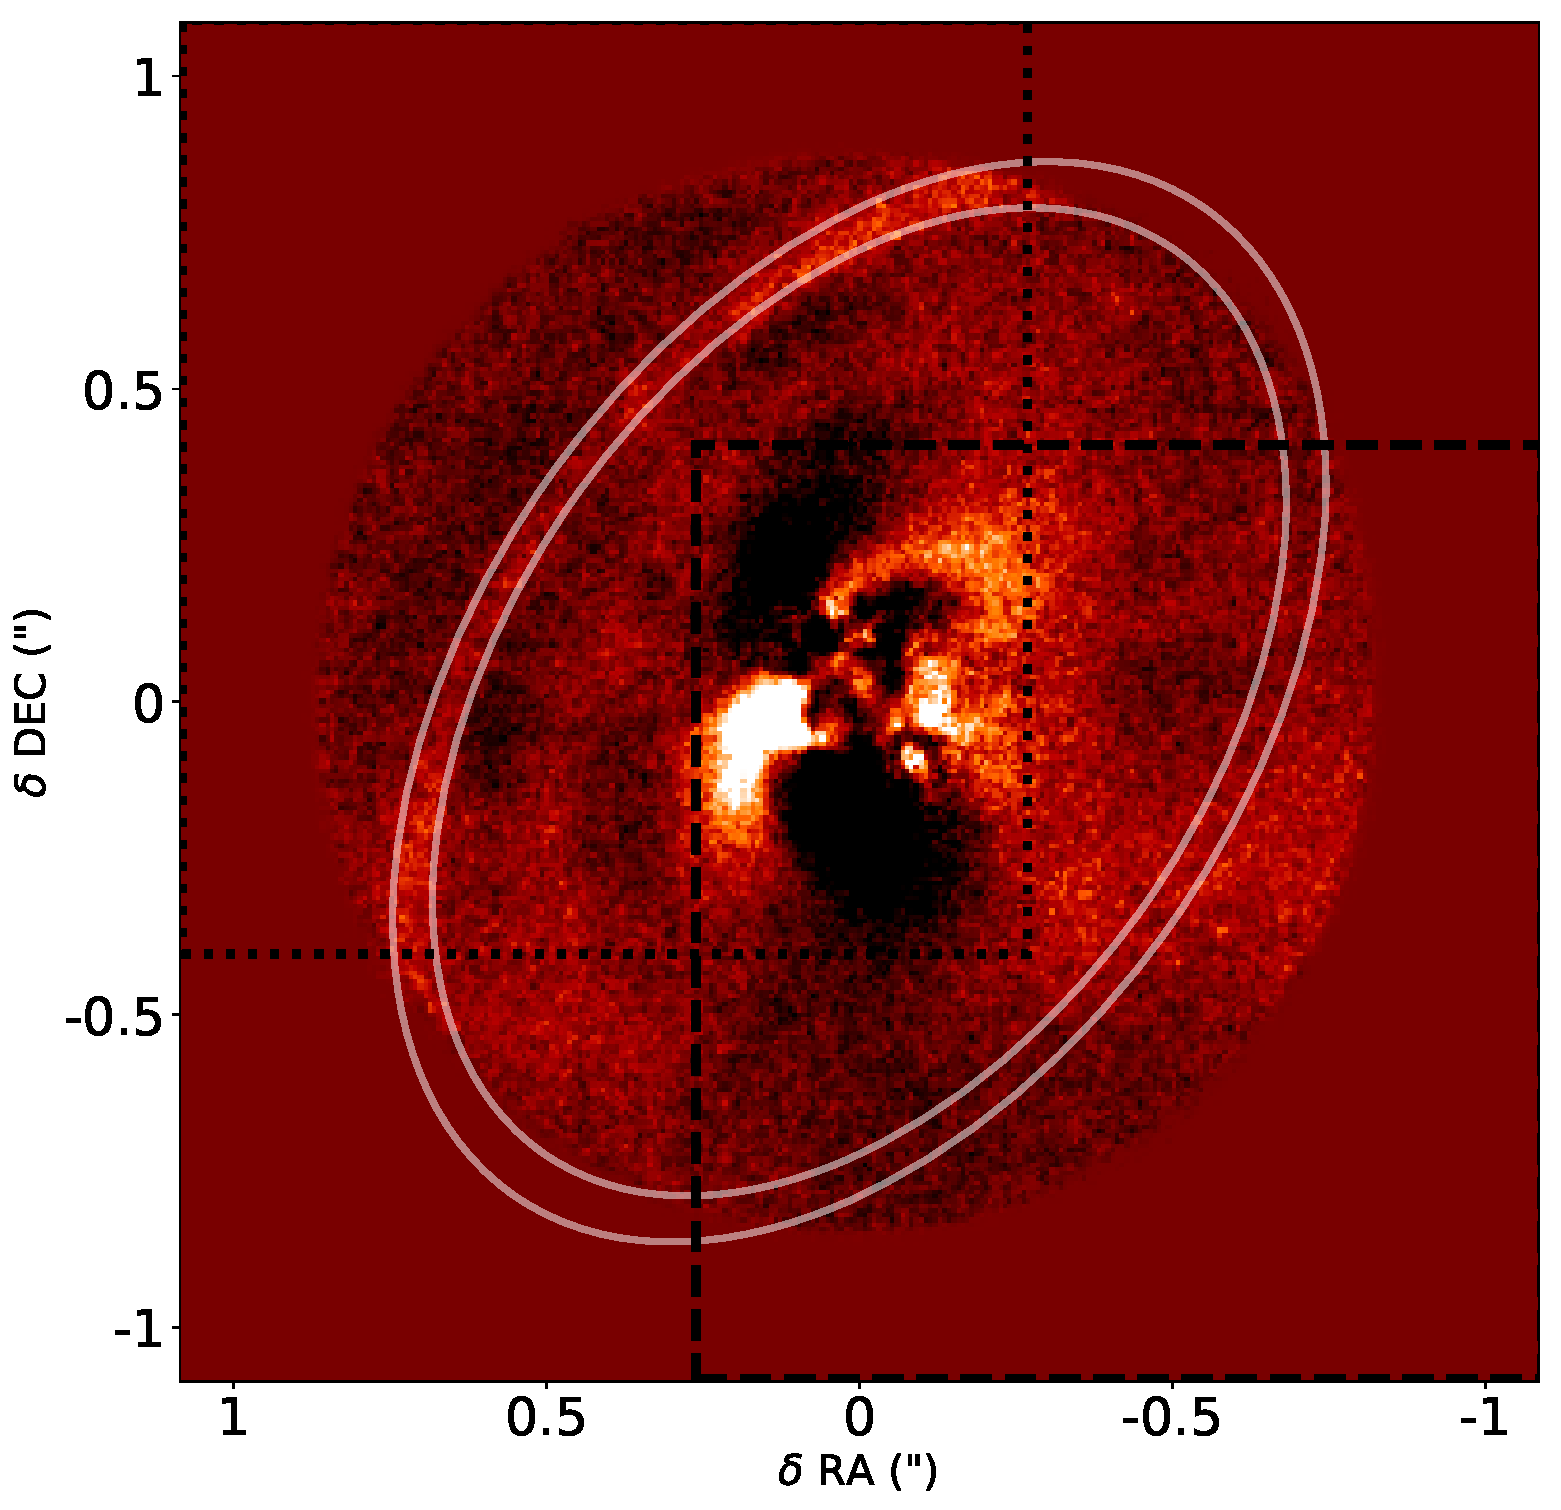
\includegraphics[width=0.8\linewidth]{totapertures}%
  \caption{The fitted ellips with semi major axis of 0.92", semi minor axis of 0.61" and a width of 0.067" together with the two masks that are used to select the region with the signal and the background region on the other side of the star.}
  \label{fig:ADIfit}
\end{subfigure}
\caption{}
%\label{fig:masterdark}
\end{figure}

One of the rings (R2 in Figure \ref{fig:irdisjos}) is well detected after the ADI reduction of the data. A fit over this ring gave an ellips with a semi minor axis of 0.61", a semi major axis of 0.92" and a full width half maximum of 0.067",rotated over $55^o$ as illustrated in Figure \ref{fig:ADIfit}. The arc just inside this ring (A2) is visible but the signal to noise ratio of this arc is not sufficient to do any analysis on this. There are some signs for a gap between A2 and the innermost disk structures. Due to the structures of the noise in that region, which is a byproduct of the ADI recipe, it is impossible to tell the exact radius where this gap is present.
\bigskip

The total amount of counts of the ring in the ADI reduction is $437\pm 10$. A same flux calculation of the region in the fit on the other side of the star, selected with a different mask as displayed in Figure \ref{fig:ADIfit}, shows an estimate of the background signal of $-6\pm 9$ counts. The background signal is close to zero as expected, it being negative is a side effect of the differential imaging. 
\bigskip

As visible in Figure \ref{fig:ADItot}, the ring gets fainter when it approaches the minor axis of the fitted ellips. This is due to selfsubtraction of the ring in the ADI routine, since the ring approaches a circular shape at that point as seen from the center of rotation.
\bigskip

The position and shape of the disk signal in the data after the ADI reduction does not change with increasing wavelength as illustrated in Figure \ref{fig:ADIcolor}. The shape of the ring and the variations in flux does not change, just as the structures in the background. The total signal of the disk however, does increase with wavelength. This variation is worked out in detail in the discussion.

\begin{figure}[htb]
\centering
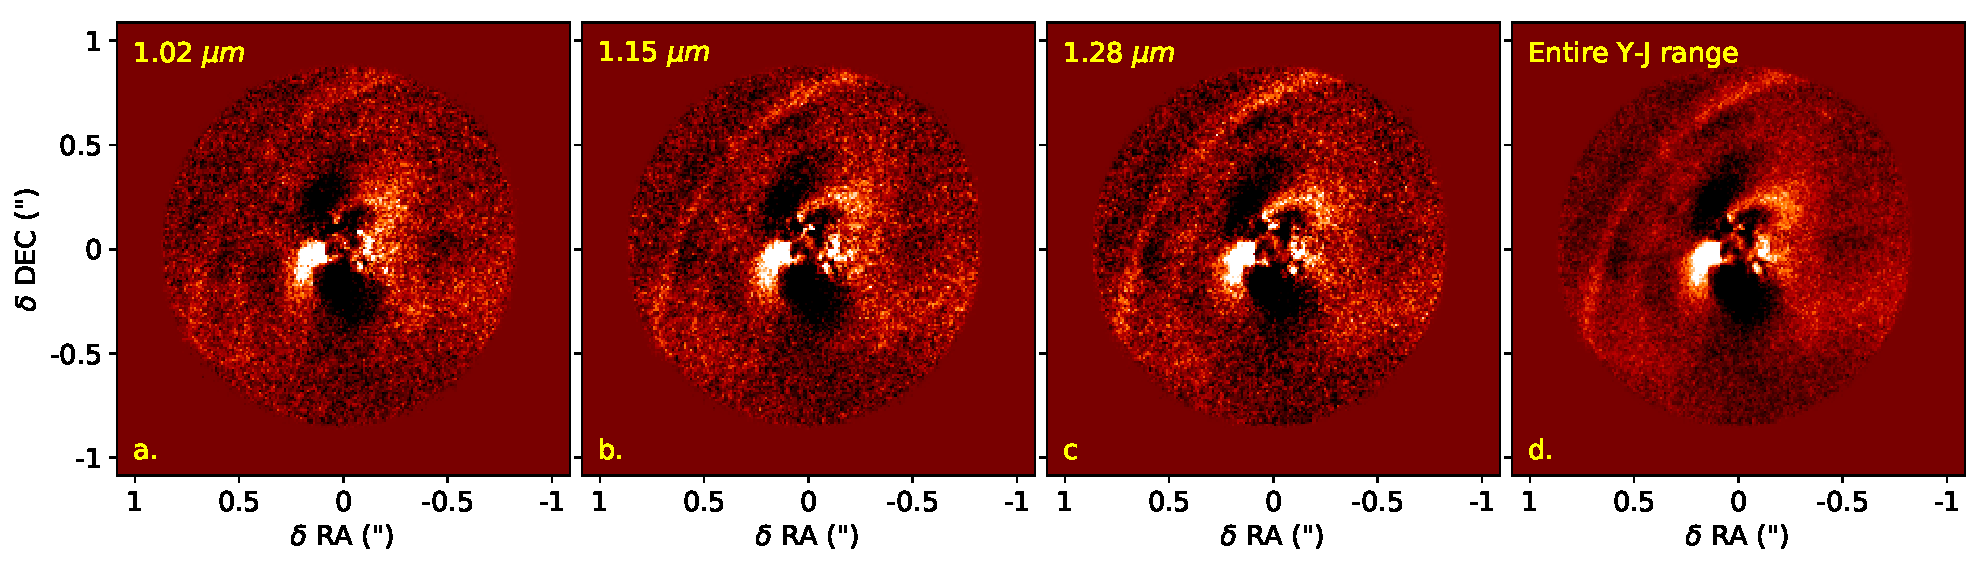
\includegraphics[trim={0cm 0cm 0cm 0cm},clip,width = \textwidth]{ADIwavelplot}
\caption{Reduction of IFS ADI data. From left to right: \textbf{a:} median of the first 13 channels (0.96-1.07$\mu m$) \textbf{b:} median of 13 channels (1.08-1.21 $\mu m$) \textbf{c:} median of 13 channels (1.22-1.33 $\mu m$) \textbf{d:} median of the entire YJ range}
\label{fig:ADIcolor}
\end{figure}

\clearpage
\section{SDI}
\begin{wrapfigure}{R}{0.5\textwidth}
\vspace{-0.5 cm}
\centering
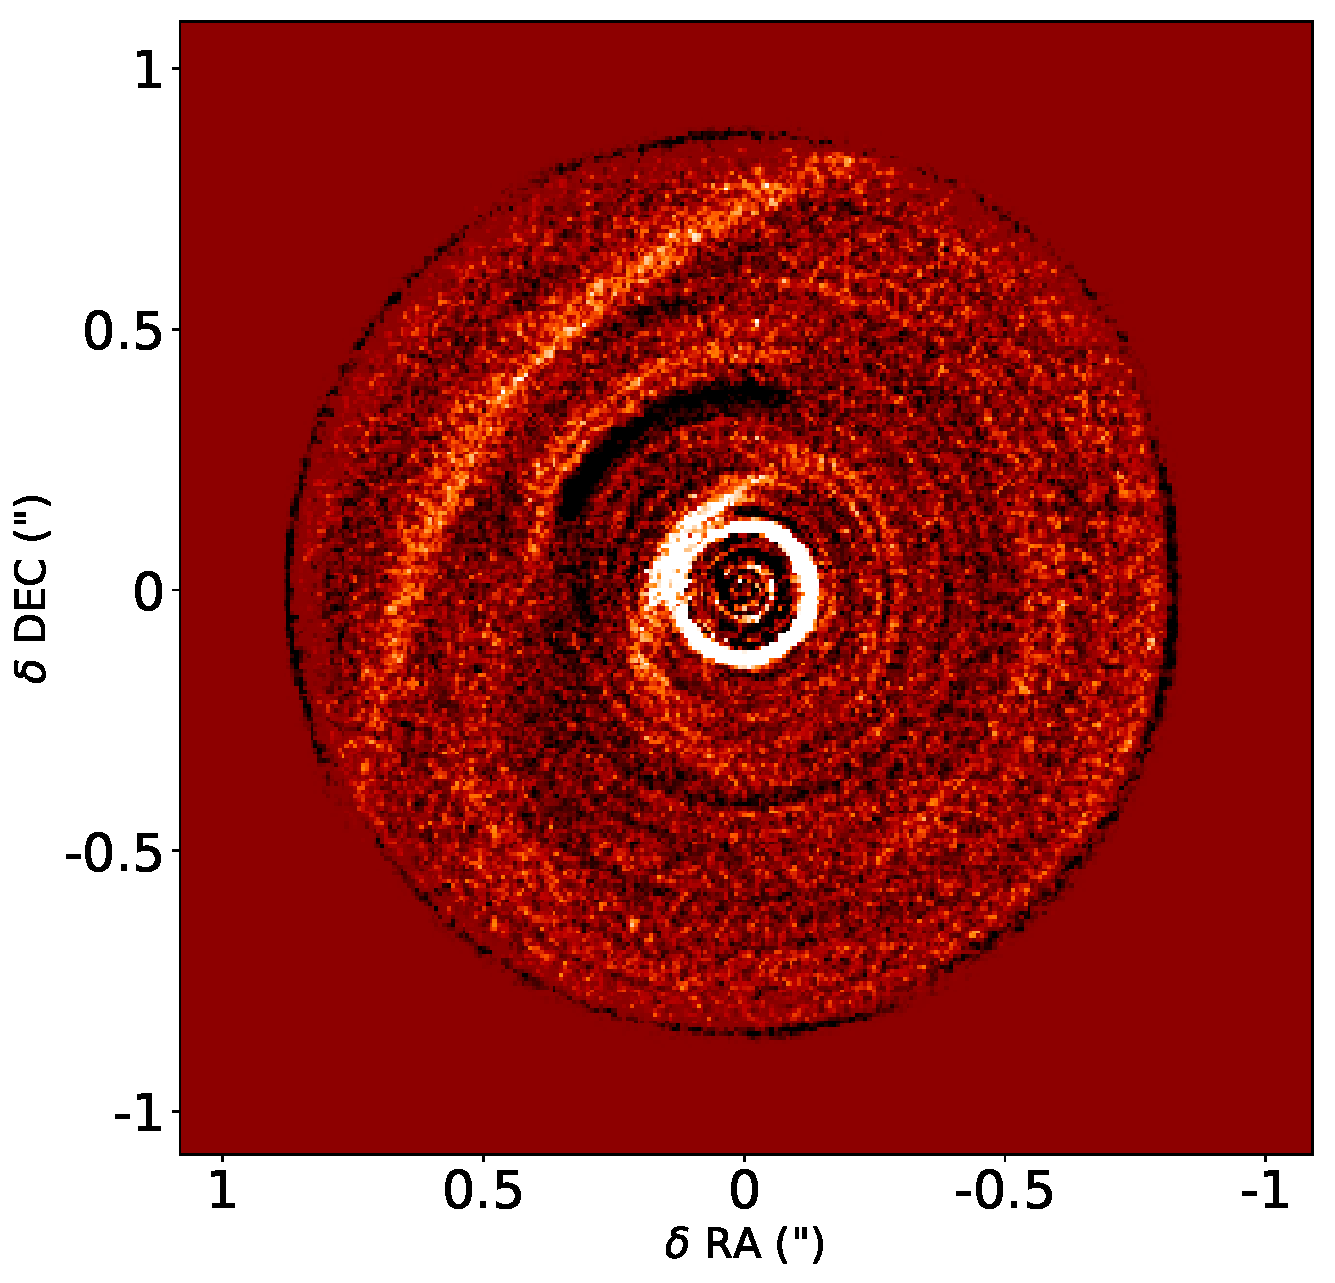
\includegraphics[width=\linewidth]{SDI_tot}
\caption{The median SDI image of all exposures over the whole Y-J wavelength range of RX J1615}
\label{fig:SDI_tot}
\vspace{-0.7 cm}
\end{wrapfigure}

The big ring (R2) that is visible after the ADI reduction is also visible after the SDI reduction. By using the same fit as after the ADI reduction, we measured the total flux of the ring after applying SDI on the data to be 644 $\pm 13$. This is a bit more than the total flux of the ring after applying ADI. The flux in the background, measured in the same annulus over the same area on the other side of the star, is 73 $\pm 11$. This is also more than after applying ADI, leaving slightly more signal of the disk in the SDI image after subtraction the total flux of the background.  
\bigskip

A2, the arc just inside R2, is visible as well, but its shape has changed with respect to the ADI reduction. This is probably due to the dark arc just inside A2, which is caused by a bad region of the detector, rotated over the different exposures. This bad region could cause a difference in the model for the PSF of the star after scaling the whole image according to its wavelength, as mentioned in chapter 4. The bad region is then smeared out over a larger region of the image, leaving some negative signal in that region for certain wavelengths before taking the median to build a model for the stellar PSF. This could cause that A2 is more prominent above the bad region and looks much more circular than after applying ADI. 
\bigskip

The innermost disk structure (I1) is much more prominent in the SDI data than in the ADI data. It is clearly visible that this has a ringlike shape over a range of almost $180^o$. The closed circular ring at an angular seperation of 0.15" is an artefact of the reduction method, probably due to the structure in the raw signal that is caused by the coronagraph, as displayed in Figure \ref{fig:reduceddata}. Furthermore, the SDI image does show much less structures in the background than the ADI image. This could either mean that these structures are created during the ADI procedure or that the SDI procedure needs a higher contrast signal to work properly.
\bigskip

From Figure \ref{fig:SDIcolor} it becomes clear that the signal of the disk increases with increasing wavelength, just as the signal after applying ADI does. The disk being positive at longer wavelengths and negative at shorter wavelengths is probably an artefact of the classical SDI routine. 

\begin{figure}[htb]
\centering
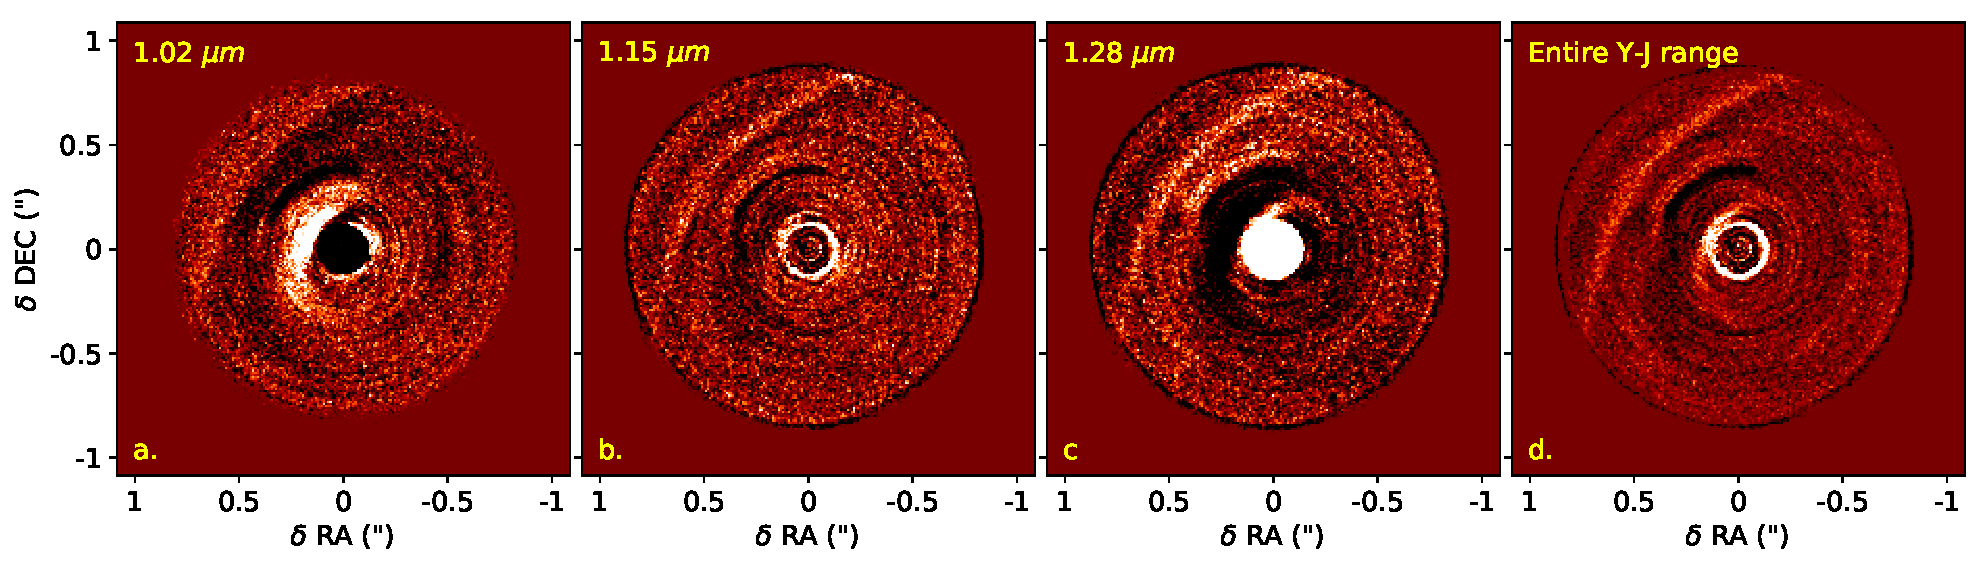
\includegraphics[trim={0cm 0cm 0cm 0cm},clip,width = \textwidth]{SDIwavelplot}
\caption{Reduction of IFS SDI data. From left to right: \textbf{a:} median of the first 13 channels (0.96-1.07$\mu m$) \textbf{b:} median of 13 channels (1.08-1.21 $\mu m$) \textbf{c:} median of 13 channels (1.22-1.33 $\mu m$) \textbf{d:} median of the entire YJ range}
\label{fig:SDIcolor}
\end{figure}

\noindent
Taking just the median over wavelength per pixel leaves some signal of the disk in the model of the PSF, causing some areas to be oversubtracted and other areas to be undersubtracted. This changes over wavelength since the signal of the disk in the model for the PSF in the SDI routine is rescaled corresponding to the wavelength.

\chapter{Spectral analysis}
\section{Morphology changes in the disk}
\begin{figure}[htb]
\centering
\includegraphics[trim={0cm 0cm 0cm 0cm},clip,width = \textwidth]{coloroverangle}
\caption{The relative flux over azimuthal angle in three different wavelength bins \textbf{a:} 13 channels (0.96-1.07$\mu m$) \textbf{b:} 13 channels (1.08-1.21 $\mu m$) \textbf{c:} 13 channels (1.22-1.33 $\mu m$) \textbf{d:} signal of the whole spectrum}
\label{fig:coloroverangle}
\end{figure}

The morphology of the disk is dependent of the reduction method that is chosen. In the ADI image as illustrated in \ref{fig:ADItot} is a clear dip in the signal visible at the point where the ring approaches the center of rotation. To quantify this change in flux in that region, we measured the flux in an apperture that is dragged over the whole ring. The apperture is circular with a radius of 0.067", as wide as the FWHM of the ring. This analysis is shown in Figure \ref{fig:coloroverangle}. This figure illustrates that the ring in the ADI image approaches zero at an azimuthal angle of about $50^o$ in the different wavelength bins. The signal in the SDI image is much more constant throughout the ring. Since the total effective flux of R2 in the SDI image is a bit higher than in the ADI image, we can conclude that part of the signal in the ADI image is selfsubtracted. This is due to the fact that the ring approaches a circular shape, which means that it shows up on the same location in each exposure. The model for the stellar PSF contains hence this part of the signal, which means that the disk signal is subtracted from the image.
\bigskip

The innermost disk structure is much better visible in the SDI image. This is due to the way ADI works. On small radii from the center of rotation, the signal has not moved enough over the detector if the field rotates with $4^o$ per exposure and the signal is distorted. This is why the structure of the disk is unclear in the ADI image. Since this structure is not that wide, it does not show up much in the model during the SDI prodecedure, which means that it looks much cleaner in the final SDI image.
\bigskip

\section{Brightness changes throughout disk}
As already visible in Figure \ref{fig:coloroverangle} and worked out further in Figure \ref{fig:coloroverpos} the signal does change over wavelength. In this figure, the flux in three different regions is plotted against the wavelength. There is a linear trend visible in both the ADI data and the SDI data. The signal in the SDI image fluctuates much over wavelength in the first region between $-10^o$ and $30^o$. This is probably due to edge effects and the unexpected negative values at shorter wavelengths, as shown in Figure \ref{fig:SDIcolor}. 

\begin{figure}[htb]
\centering
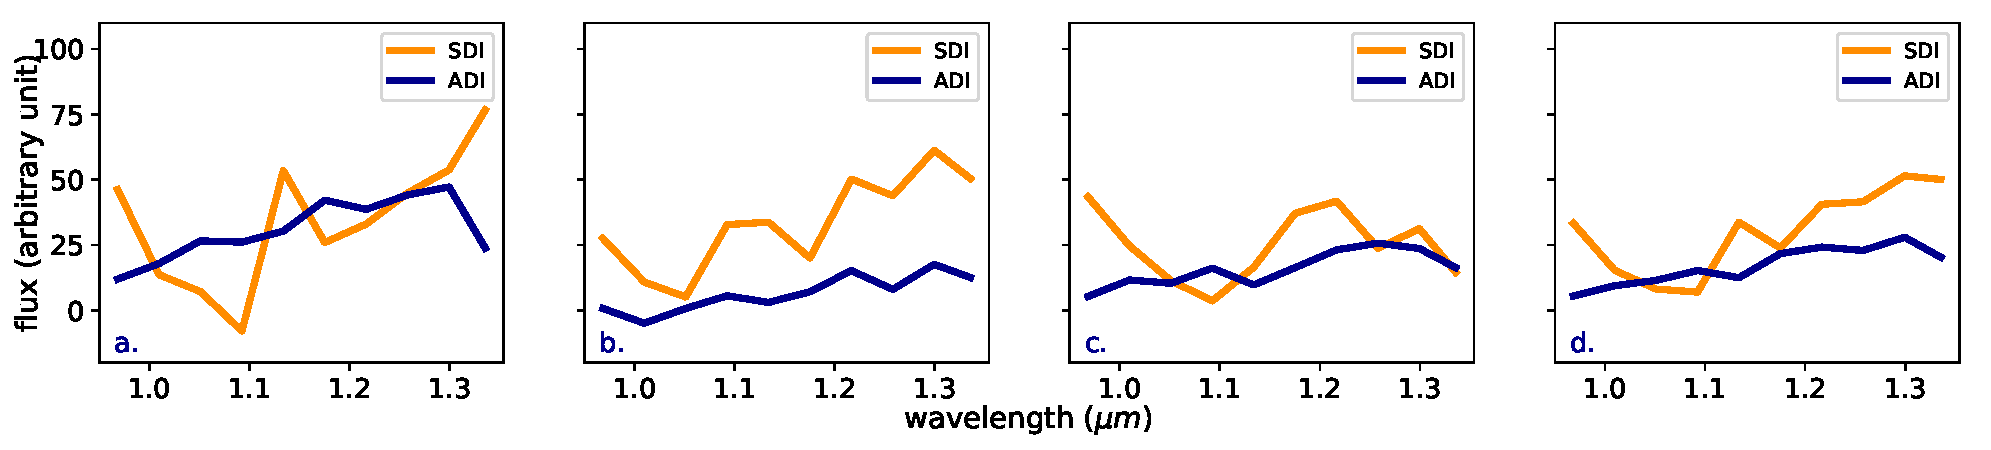
\includegraphics[trim={0cm 0cm 0cm 0cm},clip,width = \textwidth]{coloroverpos}
\caption{The relative flux of the signal over wavelength in four different regions:\textbf{a:} azimuthal angle between $-10^o$ and $30^o$  \textbf{b:} azimuthal angle between $30^o$ and $70^o$ \textbf{c:} azimuthal angle between $70^o$ and $110^o$ \textbf{d:} signal of the whole ring.}
\label{fig:coloroverpos}
\end{figure}

It is unclear if we could trust this data. The guide star is faint (R = 11.21 mag) \citep{Makarov2007}, which means that the strehl ratio in the R-band was very poor ($SR_R$ < 3\%\citep{DeBoer2016}). A poor Strehl-ratio means that the performance of SAXO is not optimal, meaning that structures can be smoothed out. Since the performance of SAXO gets better for longer wavelengths and signal is present close to R2, it is impossible to say if the increase in signal over wavelength is partly astrophysical or just an increased SAXO performance. Some signal could be washed out of the disk signal due to the low resolution. If the wavelength dependence is astrophysical, it could be caused by variations in the grain size or the chemistry throughout the disk. A good analysis of A2 and the innermost region could indicate if this change in surface brightness is astrophysical, since the surface brightness of these structures should change as well if the mechanism behind this is the increase in performance of SAXO at longer wavelengths. Radiative transfer models could be used to find an answer whether we are looking at a true astrophysical change in surface brightness with increasing wavelength or a result of the bad strehl ratio, but that is behind the scope of this project.
\bigskip

Calculating the exact error on the data points is difficult, since it is hard to determine how much of the signal is smoothed out due to the poor Strehl-ratio and how much selfsubtraction is going on during the different procedures. What we know is that the signal 

\chapter{Additional research}
After we got good results on this dataset we ran the same procedure over a dataset of HD97048, which contains many disk structures as well \citep{Ginski2016}. The signal to noise ratio for this dataset was not sufficient to detect any disk structures in both classical ADI and SDI with SPHERE/IFS.
\bigskip

After analyzing the effects on the data of the ADI and SDI procedure and investigating what we can trust out of the data, we tried also classical Reference star Differential Imaging to see what the effects of this methods are on the data. The star TYC\_7408\_0054\_1 is used as a reference model to subtract the stellar PSF from the total signal. This star is located at 18 50 44.4873 -31 47 47.332, so close to RX J1615, has spectral type K8Ve, which is close to K5D, the spectral type of RX J1615 and has an R-band magnitude of 10.745, which is close to 11.21, the R-band magnitude of RX J1615. These three parameters together with the fact that there is data of this star available that is taken in the same night as the RX J1615 dataset, make this star to be a good choice for a reference star. The throughput of the atmosphere varies over direction and time, which makes the date of the dataset and the direction of the star relevant. 
The AO system performs better at lower R-band magnitudes, which means that the R-band magnitude of the reference star has to be from the same order as RX J1615 and the spectral type has to be the same to use its PSF as a model that can be subtracted from the reduced RX J1615 dataset.
\bigskip

\begin{wrapfigure}{R}{0.465\textwidth}
\vspace{-5mm}
\centering
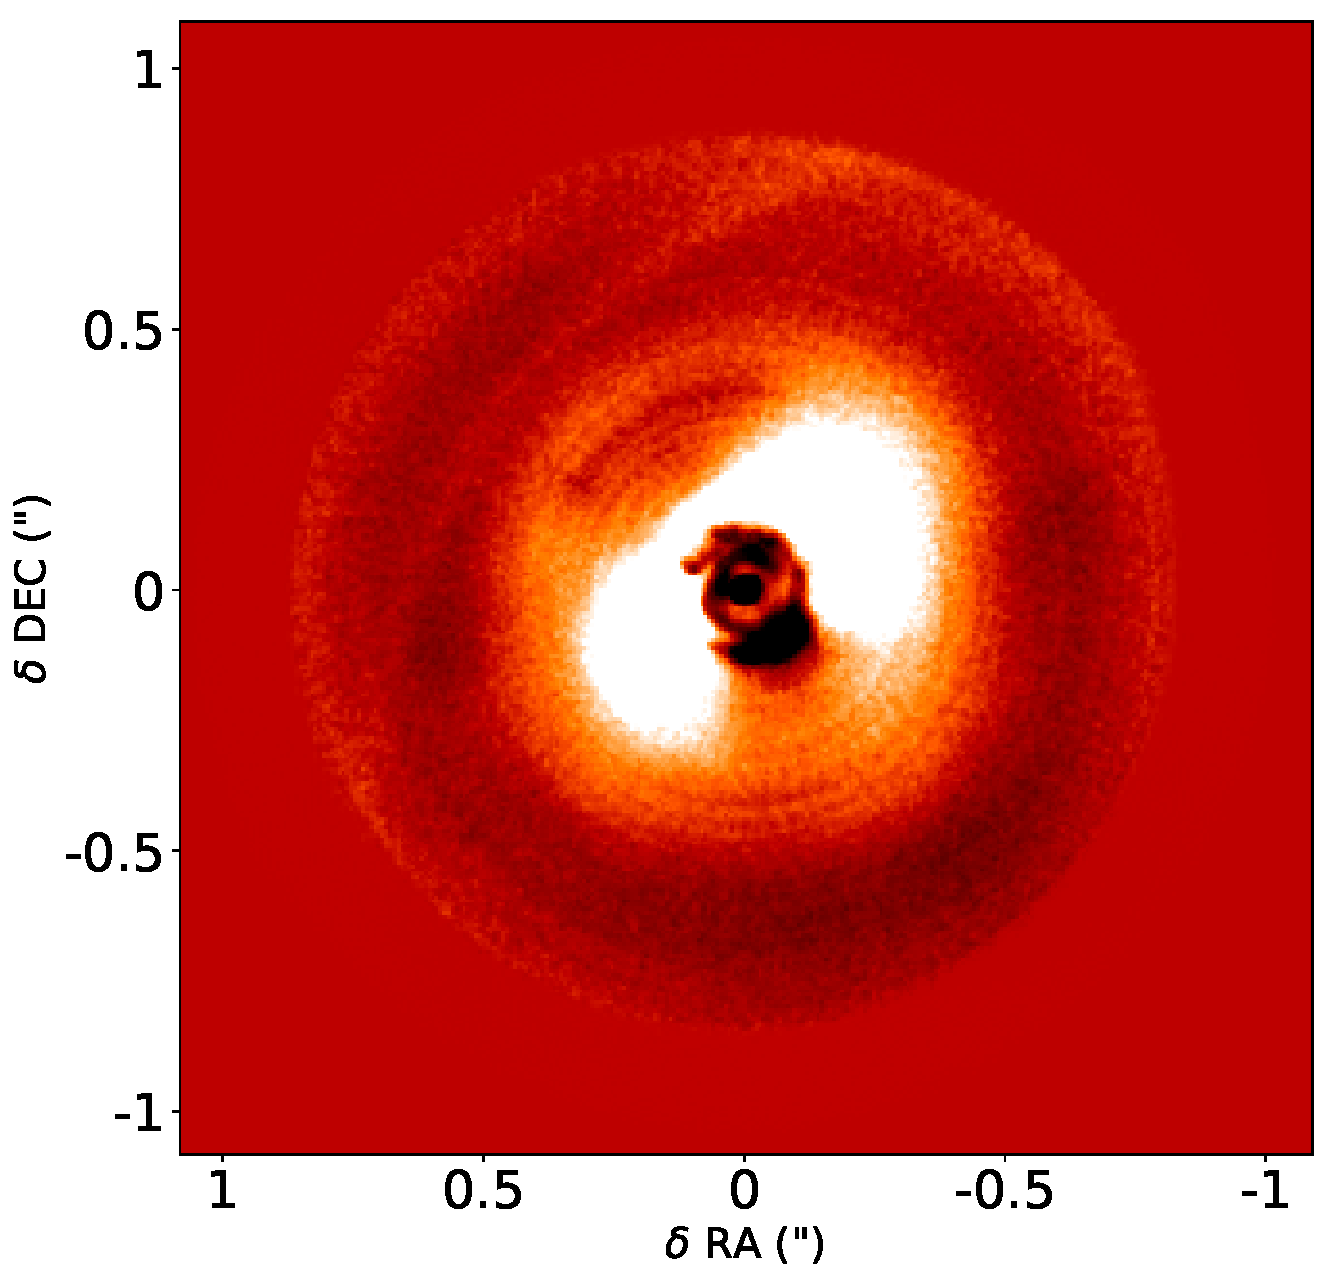
\includegraphics[width=\linewidth]{RDI_tot}
\caption{The median RDI image of all exposures over the whole Y-J wavelength range of RX J1615}
\label{fig:RDI_tot}
\vspace{-7mm}
\end{wrapfigure}

R2 is detected in the RDI image as well, as illustrated in Figure \ref{fig:RDI_tot} and has a total flux of $10943 \pm 255$ and a total flux in the background of $8881 \pm 220$. This means that this is much higher than the signal in the ADI and SDI image. For a good comparison however, is a better normalization needed between the PSF of the reference star and RX J1615. This normalization was not sufficient, since the background has such a high value, even in the regions where no disk signal is present in the ADI and SDI data.
\bigskip

Figure \ref{fig:RDIcolor} illustrates that the signal of the disk increases at longer wavelengths, just as noticed from the ADI and SDI images. The signal in the RDI image seems much more prominent at low azimuthal angles as well. This could however also be an edge effect or a result of the insufficient normalization. Additional research is needed before this could be compared in a correct way with the ADI and SDI image.

\begin{figure}[htb]
\centering
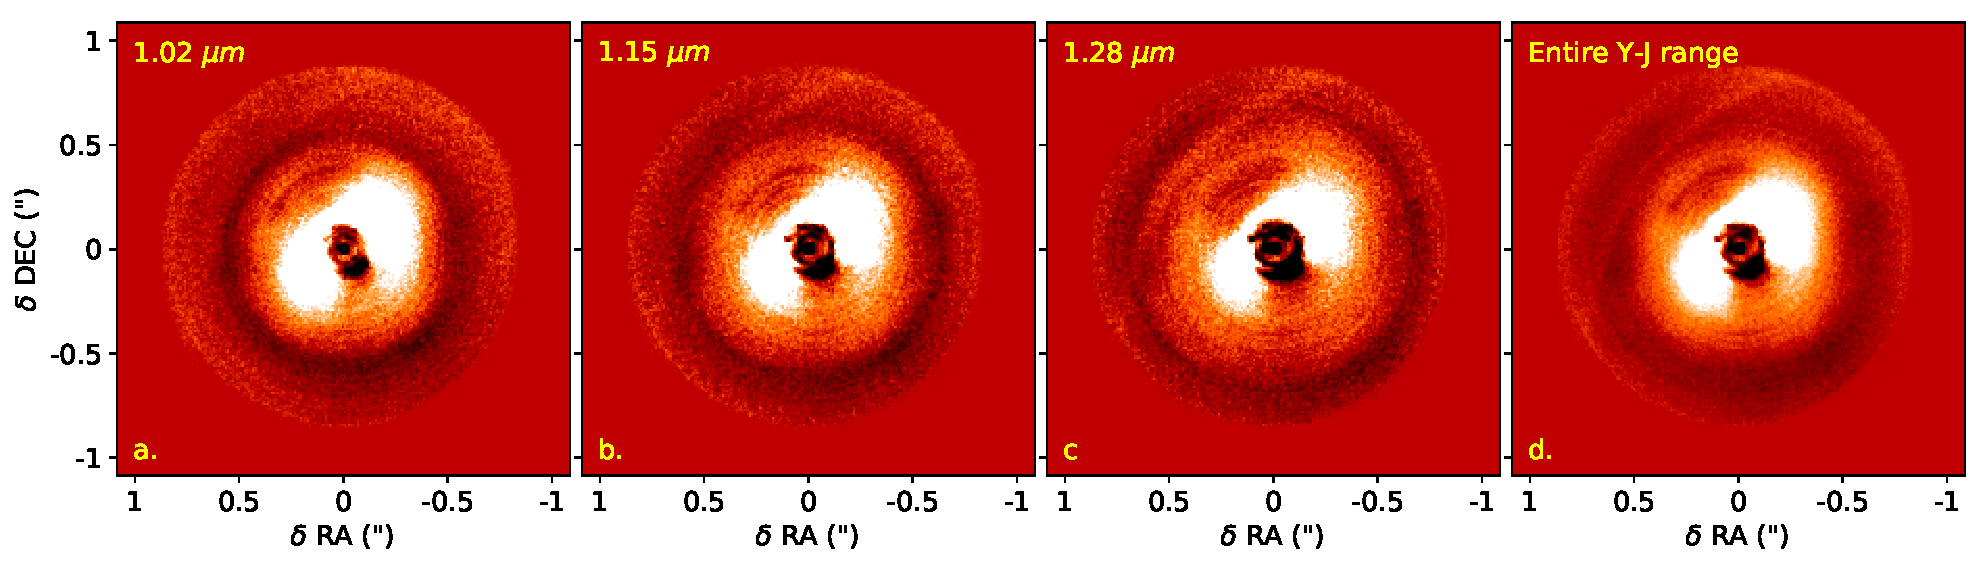
\includegraphics[trim={0cm 0cm 0cm 0cm},clip,width = \textwidth]{RDIwavelplot}
\caption{Reduction of IFS RDI data. From left to right: \textbf{a:} median of the first 13 channels (0.96-1.07$\mu m$) \textbf{b:} median of 13 channels (1.08-1.21 $\mu m$) \textbf{c:} median of 13 channels (1.22-1.33 $\mu m$) \textbf{d:} median of the entire YJ range}
\label{fig:RDIcolor}
\end{figure}

\chapter{Discussion}
\section{Comparing classical ADI with TLOCI}
Comparing the reduced image of the classical ADI as done during this research which is illustrated in Figure \ref{fig:ADIcolor} and the T-LOCI ADI reduction provided in earlier research which are illustrated in Figure \ref{fig:ADIcolor} and Figure \ref{fig:ifsjos} does not give big differences. The morphology of the clear resolved ring and the structures in the background are the same in both images and A2 is also as good detected in the classical ADI image as in the T-LOCI reduction. This means that the median of the different exposures, as created during the ADI procedure, is already a good reference for the stellar PSF and does not contain much disk signal. The reason why the more advanced reduction method T-LOCI does not make the signal of the disk beter detectable in this case is probably the amount of field rotation in the dataset. This is with $69^o$ over 16 exposures very good, meaning that there is a minimum amount of selfsubtraction going on in the dataset. This makes that the classical method used already a good model for the stellar PSF, taking all the excess signal out of the data, but leaving as much signal of the disk as possible in the final image.  

\section{Further research}
PCA
better RDI reduction
error on the wavelength dependent flux over the azimuthal angle.

\chapter{Conclusion}





\clearpage
\huge{Appendix 1: Sof files}
\small
\subsubsection*{Master dark}
\begin{mdframed}[linewidth = 0.3mm, linecolor = black]
raw/SPHER.2015-05-15T\dots.fits IFS\_DARK\_RAW
\end{mdframed}

\subsubsection*{Background calibration}
\begin{mdframed}[linewidth = 0.3mm, linecolor = black]
raw/SPHER.2015-05-15T\dots.fits IFS\_CAL\_BACKGROUND\_RAW\\
raw/SPHER.2015-05-15T\dots.fits IFS\_CAL\_BACKGROUND\_RAW
\end{mdframed}

\subsubsection*{Master detector flat}
\begin{mdframed}[linewidth = 0.3mm, linecolor = black]
raw/SPHER.2015-05-15T\dots.fits IFS\_DETECTOR\_FLAT\_FIELD\_RAW\\
raw/SPHER.2015-05-15T\dots.fits IFS\_DETECTOR\_FLAT\_FIELD\_RAW
\end{mdframed}

\subsubsection*{Instrument flat}
\begin{mdframed}[linewidth = 0.3mm, linecolor = black]
raw/SPHER.2015-05-15T\dots.fits IFS\_FLAT\_FIELD\_RAW\\
calibration/master\_dark\_short.fits IFS\_MASTER\_DARK\\
calibration/static\_badpixels.fits IFS\_STATIC\_BADPIXELMAP\\
calibration/master\_detector\_flat\_l1.fits IFS\_MASTER\_DFF\_LONG1\\
calibration/master\_detector\_flat\_l2.fits IFS\_MASTER\_DFF\_LONG2\\
calibration/master\_detector\_flat\_l3.fits IFS\_MASTER\_DFF\_LONG3\\
calibration/master\_detector\_flat\_l5.fits IFS\_MASTER\_DFF\_LONGBB\\
calibration/pdt\_wave\_calib.fits IFS\_WAVECALIB\\
calibration/pdt\_wave\_calib\_cube.fits IFS\_WAVECALIB\_CUBE
\end{mdframed}

\subsubsection*{Positioning spectra}
\begin{mdframed}[linewidth = 0.3mm, linecolor = black]
raw/SPHER.2015-05-15T\dots.fits IFS\_SPECPOS\_RAW\\
calibration/master\_dark\_short.fits IFS\_MASTER\_DARK\\
calibration/static\_badpixels.fits IFS\_STATIC\_BADPIXELMAP
\end{mdframed}

\subsubsection*{Wavelength calibration}
\begin{mdframed}[linewidth = 0.3mm, linecolor = black]
raw/SPHER.2015-05-04T\dots.fits IFS\_WAVECALIB\_RAW\\
calibration/master\_dark\_short.fits IFS\_MASTER\_DARK\\
calibration/static\_badpixels.fits IFS\_STATIC\_BADPIXELMAP\\
calibration/spectra\_positions.fits IFS\_SPECPOS
\end{mdframed}

\subsubsection*{Science reduction}
\begin{mdframed}[linewidth = 0.3mm, linecolor = black]
raw/SPHER.2015-05-15T\dots.fits IFS\_SCIENCE\_DR\_RAW\\
calibration/master\_dark\_long.fits IFS\_MASTER\_DARK\\
calibration/static\_badpixels.fits IFS\_STATIC\_BADPIXELMAP\\
calibration/master\_detector\_flat\_l1.fits IFS\_MASTER\_DFF\_LONG1\\
calibration/master\_detector\_flat\_l2.fits IFS\_MASTER\_DFF\_LONG2\\
calibration/master\_detector\_flat\_l3.fits IFS\_MASTER\_DFF\_LONG3\\
calibration/master\_detector\_flat\_l5.fits IFS\_MASTER\_DFF\_LONGBB\\
calibration/pdt\_wave\_calib.fits IFS\_WAVECALIB\\
calibration/pdt\_wave\_calib\_cube.fits IFS\_WAVECALIB\_CUBE\\
calibration/ifs\_instrument\_flat.fits IFS\_INSTRUMENT\_FLAT\_FIELD\\
calibration/ifs\_ifu\_flat.fits IFS\_IFU\_FLAT\_FIELD
\end{mdframed}

%\chapter*{Appendix 2: Workflow}
\clearpage
\huge{Appendix 2: Workflow}
\begin{figure}[ht]
\vspace{-2cm}
\centering
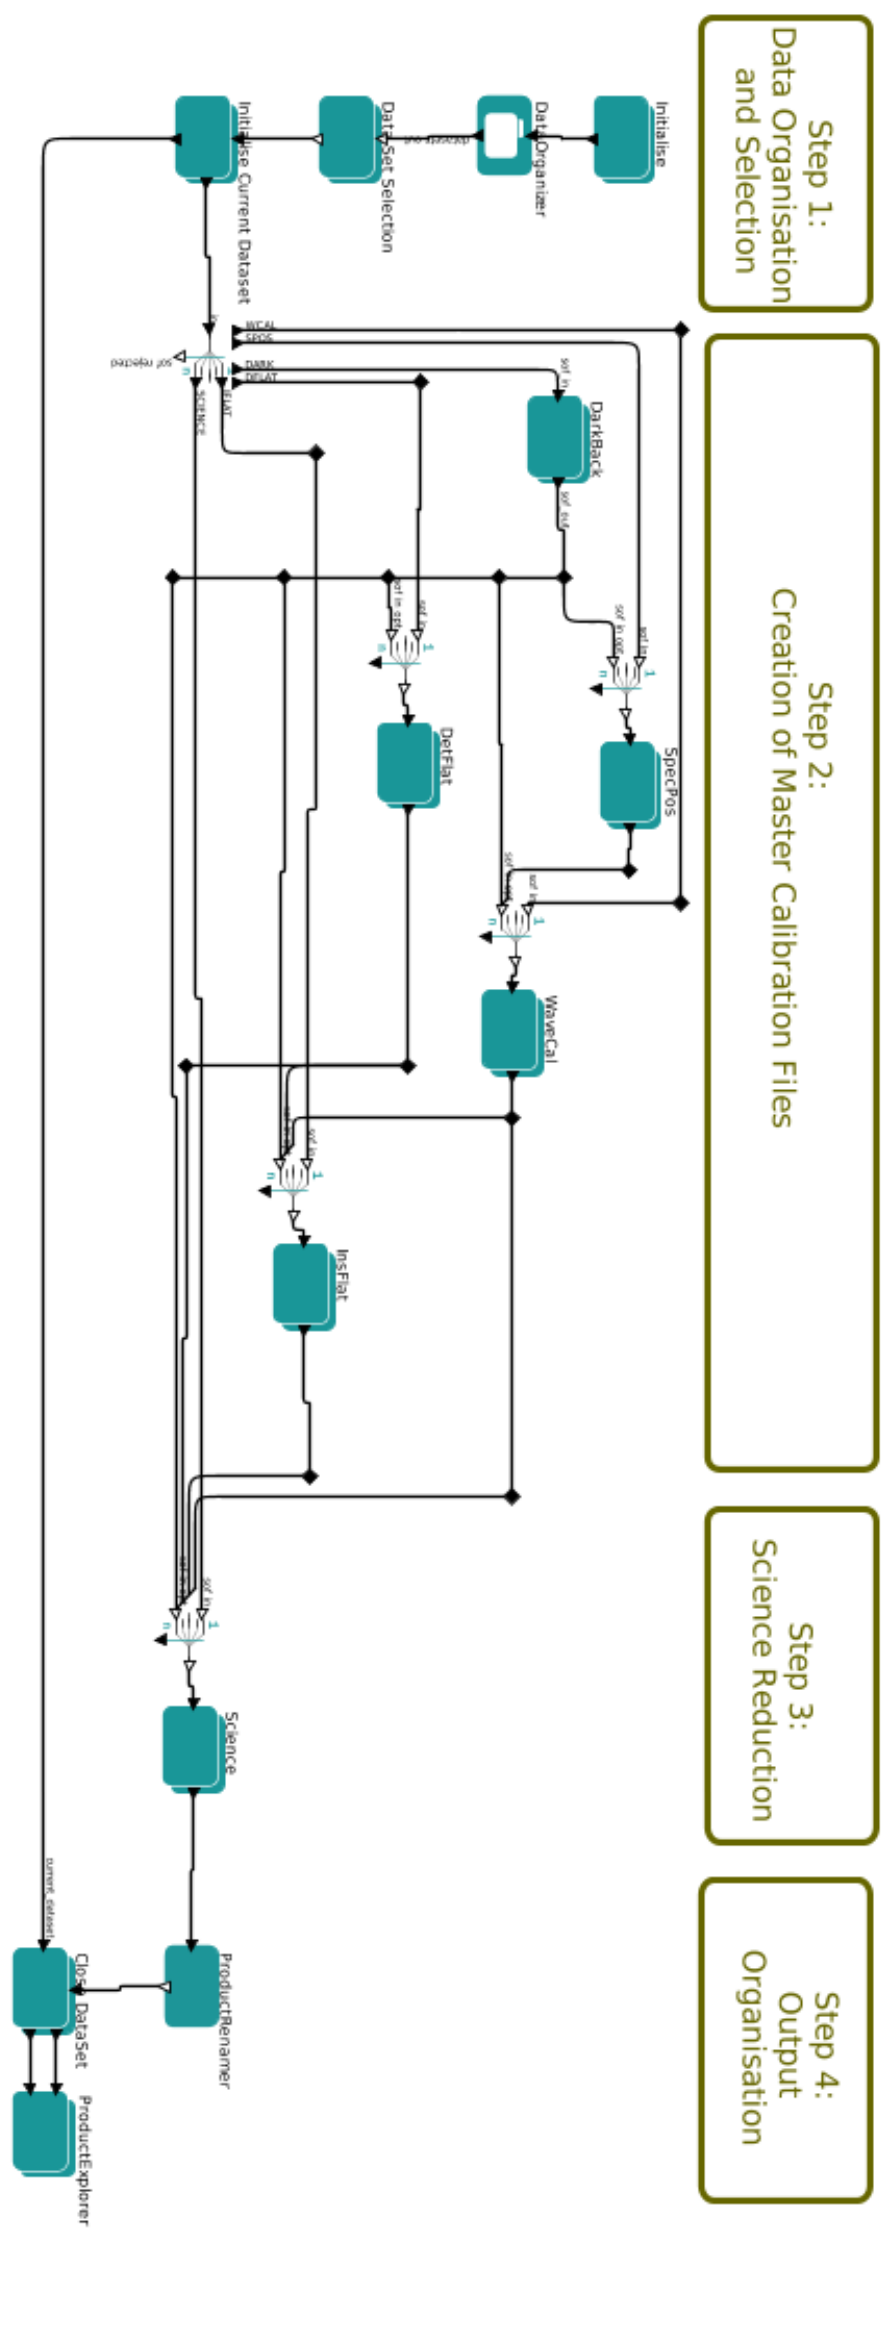
\includegraphics[height = 0.95\textheight]{workflow}%
\vspace{-2cm}
%\caption{}
%\label{fig:workf}
\end{figure}%

%\clearpage


%\include{soffiles}
%\appendix
%\include{appa}

\section*{Acknowledgements}
\small
This research was made possible by financial support from the Dutch Association for Scientific Research (NWO) and the Foundation for Fundamental Research of Matter (FOM).





%\nocite{Brandt2013}*}
\bibliographystyle{lion-msc}
\bibliography{BRP}

\clearpage
\subsection*{Reference star differential imaging}
Reference star differential imaging (RDI) is a calibration technique that uses the point spread function (PSF) of a similar star as the observed object, without a disk. The PSF from the hosting star is static, so if this could be subtracted, the contrast between the star and the disk is much bigger. It is hard to find a reference star that has been observed in the same mode, in the same period and with the same conditions. All these things can change the PSF drastically, which means that it is impossible to subtract the PSF of reference star. The reference star also has to have about the same spectrum, in order to deal properly with the luminosity difference in different wavelength bins of the different spectral types and the fact that the IFS takes data over a range of wavelengths. 
\bigskip

The distorted wavefront that has to be corrected by the adaptive optics of the VLT is measured in the R-band filter. The extreme adaptive optics of the VLT is very sensible and slightly magnitude dependend, which just means that the adaptive otics work better if a brighter object is observed. Consequence of this, is that the reference star to apply RDI, has to be the same order of magnitude in the R band as the observed object. A different performance of the adaptive optics, can change the PSF such that it is not suitable for reference star subtraction anymore. 

\end{document}

